\def\CPL{\E|C|\xspace}
\def\CPL{\E|C|\xspace}
\renewcommand\lisp[1]{{\renewcommand \codesize {\normalsize} \lstinline[language=Mini]{#1}}}
%%%%%%%%%%%%%%%%%%%%%%%%%%%%%%%%%%%%%%%%%%%%%%%%%%%%%%%%%%%%%%%%%%%%%%%%%%%%%%%
% Code for collecting code exerpts into a separate library and kernel files
%%%%%%%%%%%%%%%%%%%%%%%%%%%%%%%%%%%%%%%%%%%%%%%%%%%%%%%%%%%%%%%%%%%%%%%%%%%%%%%
\newcounter{kernel}
\newcounter{library}
\setcounter{library}0

\newread \tempFile % A temporary reading stream
\newwrite \kernelFile % A stream to save kernel functions
\newwrite \libraryFile % A stream to save library functions
\immediate \openout \kernelFile=\jobname.kernel.lisp
\immediate \openout \libraryFile=\jobname.library.lisp

% An environment for writing kernel functions
\newenvironment{KERNEL}{%
  \stepcounter{kernel}
  \def\fileName{\jobname.kernel.\arabic{kernel}.lisp}%
  \global\let\savedifeof=\ifeof
  \def\ifeof##1{\global\let\ifeof=\savedifeof\iftrue}%
  \csname filecontents*\endcsname{\fileName}%
}{%
  \csname endfilecontents*\endcsname%
  \pagebreak[3]%
  \LTR
  \lstinputlisting[language=Mini,style=display,backgroundcolor=\color{olive!10}]{\fileName}%
  \endLTR
  \pagebreak[3]%
  \openin\tempFile=\fileName
  \begingroup\endlinechar=-1%
  \loop\unless\ifeof \tempFile
  \read\tempFile to\fileline % Read one line and store it into \fileline
  \ifeof\tempFile\else{
    \immediate\write\kernelFile {\unexpanded\expandafter{\fileline}}%
   }\fi
  \repeat
  \endgroup
  \closein \tempFile
}

% An environment for writing library functions
\newenvironment{LIBRARY}{%
  \stepcounter{library}
  \def\fileName{\jobname.library.\arabic{library}.lisp}%
  \global\let\savedifeof=\ifeof
  \def\ifeof##1{\global\let\ifeof=\savedifeof\iftrue}%
  \csname filecontents*\endcsname{\fileName}%
}{%
  \csname endfilecontents*\endcsname%
  \pagebreak[3]%
  \LTR
  \lstinputlisting[language=Mini,style=display,backgroundcolor=\color{orange!20}]{\fileName}%
  \endLTR
  \pagebreak[3]%
  \newread \tempFile % open the file to read from
  \openin \tempFile=\fileName
  \begingroup\endlinechar=-1
  \loop\unless\ifeof \tempFile
  \read\tempFile to\fileline % Read one line and store it into \fileline
  \ifeof \tempFile \else
    \immediate \write \libraryFile {\unexpanded\expandafter{\fileline}}%
   \fi
  {\unexpanded\expandafter{\fileline}} % print the content to copy.txt
  \repeat
  \endgroup
  \closein \tempFile
}%

\newcommand{\TopAlign}[1]{\adjustbox{valign=t}{#1}}
\newcolumntype{T}{>{\collectcell{\TopAlign}}c<{\endcollectcell}}
{%
    \makeatletter
    \catcode13=13\relax% Make ASCII 13 active to define it later
    \gdef\fixNewLine{%
        \def^^M{\space}%
    }%
}


\lstset{%
  rangeprefix=\{,rangesuffix=\},
%  language=Chic,
  style=display,
  backgroundcolor=\color{RoyalBlue!10},
  includerangemarker=false,
}

\lstdefinelanguage{Chic}{
  language=C++,
  deletecomment=[s]{/*}{*/},
  keywords=[3]{Integer},
  keywords=[2]{Var, Let},
  keywords=[1]{goto,try,catch,return},
  escapeinside={/**}{*/},
  escapebegin={/** \bgroup\fixNewLine\renewcommand\baselinestretch{1.1}
  \commentsfont\normalsize\color{commentColor!40!black}\slshape},
  escapeend={\egroup*/}
}

\begin{LTR}
  \def\codesize{\small}
  \lstinputlisting[linerange=REPL-END,language=Chic,backgroundcolor=\color{white}]{Mini-Lisp.Chic/repl.cc}
\end{LTR}
\end{document}
§ מבוא

§§ מחשבים עתיקים ולידתה של ליספ

שפת LISP (ראשי תיבות דו- וארבע שלביים של \E|LIst ProceSsing|), הייתה, יחד עם
שפת Fortran (ראשי תיבות תלת- ודו-שלביים של \LR{FORmula TRANslation}), אחת משתי
שפות התכנות העיליות הראשונות. פיתוחה של ליספ החל באוניברסיטת MIT לפני יותר
משישים שנה בהובלתו של ג'ון מקארת'י (\E|McCarthy|), מחלוצי הבינה המלאכותית.

שנים רבות לאחר מכן, יתקשה מקארת'י להיזכר מתי בדיוק הופעלה ליספ לראשונה, אך ידוע
כי ב-1960 הגירסה ראשונה של ליספ, \E|LISP~I| שמה, כבר שימשה ליישומי חשבון
דיפרנציאלי ואינטגרלי, תיאוריה של מעגלים חשמליים, לוגיקה מתימטית ובינה מלאכותית.
עוד ידוע כי המאמץ למימוש השפה החל בשנת 1958. כבר באותה שנה הציג מקארת'י לראשונה
מזכר המתאר את ליספ, לא כשפת תכנות, אלא כתחשיב מתמטי לתיאור "הגיוני"
(\E|"sensible”|) של אלגוריתמים. תחשיב זה של מקארת'י התבסס על תחשיב מתימטי אחר:
תחשיב ה-$λ$ \E|(lambda calculus)| שפיתח אלונזו צ'רץ' (\E|Church|) בשנת 1936.

בימים ההם נדרש מאמץ משמעותי כדי לממש את התחשיב המתימטי של מקארת'י כשפת תכנות
הפועלת על מחשב: תכניות נכתבו אז בשפת מכונה, הוזנו למחשב על כרטיסים מנוקבים,
והפלט שלהן התקבל על מדפסות איטיות. המחשב המתקדם ביותר באותה עת היה \E|IBM~704|,
מחשב הבנוי משפופרות ריק (מאלו שאפשר לראות במכשירי טלוויזיה ורדיו עתיקים), מחשב
שתפס אמנם אולם שלם, אך גודל הזיכרון שעמד לרשותו היה פחות מ-20 קילובית, והוא היה
איטי בכמעט פי עשרת אלפים מטלפון סלולרי מיושן כדוגמת \E|Samsung~S2|.

לעומת זאת, לא היה קשה לממש את ליספ באמצעות עצמה. מקארת'י הציג לראווה את כוחה
של ליספ בכך שכתב בה פונקציה (רקורסיבית אמנם, אך רחוקה מלהיות מסובכת),
\begin{equation} \label{eq:eval}
  \text{eval}(ℓ, a),
\end{equation}
אשר קיבלה כפרמטר תכנית ליספ כלשהי~$ℓ$, וביצעה את~$ℓ$ תוך שימוש ב-$a$, הפרמטר
האחר ל-\E|eval|, כ-"סביבה" שבה יש לבצע את~$ℓ$. הסביבה היא רשימת ההגדרות בהן~$ℓ$
יכולה להשתמש. לשם ביצוע תכנית נתונה~$ℓ$, יש להפעיל את-\E|eval| על~$ℓ$
ועל~$a$ המציין רשימת הגדרות ריקה. הפעלות רקורסיביות של \E|eval| תהיינה על חלקים
שונים של~$ℓ$, ועל רשימת ההגדרות אשר נוצרו במהלך החישוב, שהרי יצירה זו מתרחשת כל
אימת שמועברים ארגומנטים בקריאה לפרוצדורה או לפונקציה: שם הפרמטר מוגדר להיות
ערכו של הארגומנט.

מקארת'י הראה שכאשר \E|eval| מופעלת על תכנית~$ℓ$ ועל סביבה ריקה היא
תבצע את~$ℓ$ ממש כפי שמימוש של ליספ על מחשב היה מבצע אותה. דא עקא, שמימוש כזה
טרם היה בנמצא, ובנייתו הייתה רק בראשיתה: החוקרים שעמלו על כך עדיין תהו
כיצד ניתן לממש את ליספ כך שתוכל לרוץ באופן סביר על תשתית המחשוב הרעועה שעמדה
לרשותם. כך למשל, מדי כשמונה שעות בממוצע היה המחשב מושבת לתיקון עקב כשל באחת
מבין שפופרות הריק מהן הוא בנוי. על כך נוספה בעית קצב העיבוד שהיה איטי כל כך
שהמהדר (אשר כבר מומש) של פורטרן לא תמיד הצליח לסיים את פעולתו טרם שיוזעק טכנאי
לתיקון תקלה שהתגלתה במחשב.

מסיבה זו, הצעדים הראשונים במימוש של ליספ היו בגדר גישושים: החוקרים נהגו לבחור
תכניות ליספ קצרות, לתרגם אותן ידנית לתכניות בשפת מכונה, ולבחון את דרך פעולתם של
התרגומים שנוצרו. פריצת הדרך חלה כאשר אחד החוקרים, סטיב ראסל (\E|Russel|),
הבחין שניתן להשתמש בפונקציה \text{eval} שכתב מקארת'י כדי לממש את ליספ על מחשב
של ממש. במקום לבנות מימוש כללי של ליספ, כזה המסוגלת להתמודד עם \ע|כל| תכנית
ליספ כלשהי, מספיק לממש תכנית ליספ \ע|אחת|, הלא היא הפונקציה \E|eval|!

בליספ, כל תכנית היא פונקציה, וכל פונקציה היא תכנית. הפונקציה \E|eval| היא לכן
תכנית המסוגל לטפל בכל תכנית ליספ שהיא. ראסל תרגם את הפונקציה \E|eval| מליספ
לשפת מכונה, ואחר כך השתמש בתרגום זה והוסיף עליו מעט כדי לממש את ליספ. המימוש
היה כ\ע|אינטרפרטר|: תכנית הקוראת שורה מהקלט, מפרשת אותה כתכנית ליספ, מבצעת
אותה ומדפיסה את תוצאת החישוב.

\begin{figure}[H]
\centering
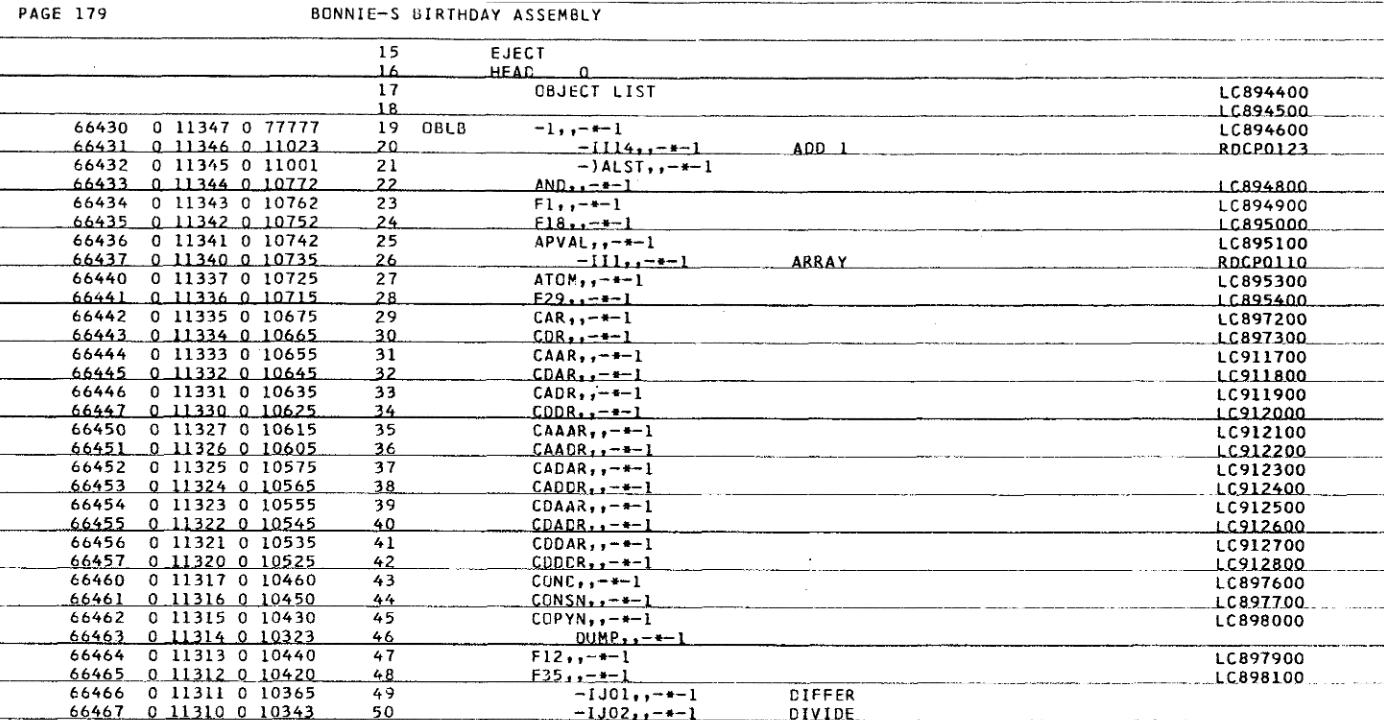
\includegraphics[width=0.45\textwidth]{lisp-assembler2}
\qquad
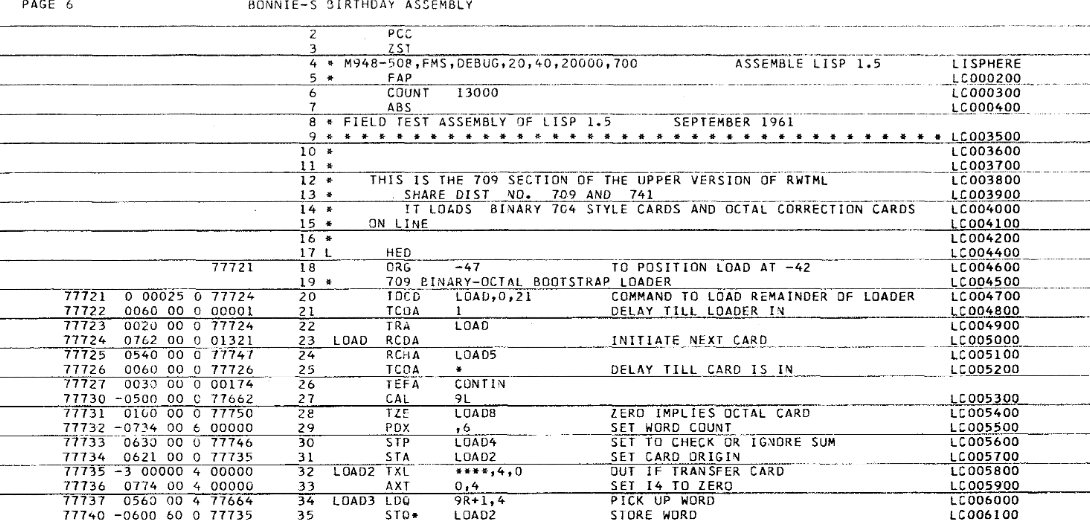
\includegraphics[width=0.45\textwidth]{lisp-assembler1}
\כיתוב|קטע מהתכנית בשפת מכונה שמימשה לראשונה את ליספ|
\תגית|איור:מימוש|
\end{figure}

\פנה|איור:מימוש| מציג קטע מהתכנית בשפת מכונה שנכתבה על ידי ראסל וחבריו כדי לממש
את eval ובאמצעותה את ליספ.

§§ \RL{נסיקתה (וצניחתה) של ליספ}

לאחר מימושה, זכתה ליספ לענין גובר והולך: מתכנתים רבים העדיפו את האלגנטיות
והתמציתיות של ליספ, על פני המסורבלות של שפת פורטרן ושפות תכנות אחרות, ולו גם
במחירה של יעילות, שכן מעצם טיבה כשפה שאינה יכולה לעבור הידור מלא, הרצה של
תכניות בליספ איטית יותר מאשר, תכניות שתורגמו משפה עילית לשפת מכונה.

\lstdefinestyle{interaction}{%
  style=display,
  frame=none,
  language=Pascal,
  backgroundcolor=\color{purple!10},
  deletekeywords={to,do,of,and,then,for},
}

בשנות השישים והשבעים שימשה השפה לפיתוחן של כמה תכניות פורצות דרך, אשר עירבו בהן
מידה זו אחרת של בינה מלאכותית: למשל,מאקסימה (\E|Macsyma| ואחר כך \E|Maxima|)
הייתה התכנית הראשונה לחישוב מתמטי סימבולי (ולא נומרי) כגון חישובי נגזרות
ואינטגרלים או פתרון של משוואות דיפרנציאליות. למשל, חישוב במקסימה של האינטגרל
הלא מסוים
\begin{equation}
  \label{eq:indefinite}
  ∫\sin³(x)\, dx=\frac{\cos³(x)}3- \cos(x)
\end{equation}
ואת האינטגרל המסוים
\begin{equation}
  \label{eq:definite}
  ∫₀^π e^x\cos²(x),dx=\frac{3 (e^π-1)}{5}
\end{equation} נעשה זאת כמתואר ב\פנה|איור:מאקסימה|.

\begin{figure}[H]
\begin{LTR}
  \lstinputlisting[style=interaction]{maxima.txt}
\end{LTR}
\כיתוב|שימוש במאקסימה לצורך חישוב האינטגרל הלא
מסוים~$∫\sin³(x)\,dx=\frac{\cos³(x)}3-\cos(x)$ והאינטגרל
המסוים~$∫₀^π e^x\cos²(x),dx=\frac{3(e^π-1)}{5}$|
\תגית|איור:מאקסימה|
\end{figure}
השיח בין המשתמש ומאקסימה באיור נפתח בסידרת התווים
\begin{LTR}
\begin{lstlisting}[style=interaction,backgroundcolor=\color{white}]
(%i1)
\end{lstlisting}
\end{LTR}
סידרה זו היא היא ה\ע|זרז| (\E|prompt|) שמציגה תכנת מאקסימה למשתמש בה: בהצגת
הזרז,  מתבקש המשתמש  להזין ביטוי מתימטי עליו מאקסימה נדרשת לפעול. ביטוי זה יסומן
כקלט מספר~1, ומכאן הכתיב
(\lisp{i1}). 


הביטוי שמזין המשתמש בתגובה לזרז הוא \E|\lisp{integrate(sin(x)³,x)}| הוא
האינטגרל אותו על מאקסימה לחשב. בתגובה, מחשבת מאקסימה את האינטגרל, ומדפיסה אותו,
תוך שהיא מסמנת אותו ב-
\begin{LTR}
\begin{lstlisting}[style=interaction,backgroundcolor=\color{white}]
(%o1)
\end{lstlisting}
\end{LTR}
 כלומר פלט מספר~1. חישוב האינטגרל~$∫₀^πe^x\cos²x\,dx$ נעשה אחר כך, כאשר הקלט
 והפלט מסומנים כמספר~2.

ישום בינה מלאכותית מובהק בליספ הוא "אלייזה" (\E|ELIZA|), תכנית המחשב הראשונה
שהייתה מסוגלת לנהל שיח עם משתמש בדומה לצ'אטבוט מודרני. אלייזה ניסתה לדמות בשיחה
את תפקיד הפסיכיאטר או הפסיכותראפיסט ודו-שיח עמה נראה, לדוגמה, כמופיע
ב\פנה|איור:אלייזה|.

\begin{figure}[H]
\begin{LTR} \scriptsize
  \lstinputlisting[style=interaction]{ELIZA.txt}
\end{LTR}
\כיתוב|קטע משיחה בין תכנת אלייזה ובין משתמש|
\תגית|איור:אלייזה|
\end{figure}

ELIZA הייתה כה מוצלחת כצ'אט בוט, שכמה מהמשוחחים עמה נפתו לחשוב שהם משוחחים עם
פסיכיאטרית היושבת במקום אחר ומשוחחת עימם באמצעות המחשב.

שפת ליספ שימשה גם לפיתוח \E|DART|, תכנת לוגיסטיקה של משרד הבטחון האמריקאי, אשר
ניהלה את שינוע של הכוחות, הציוד והתחמושת במבצע סופת המדבר (\E|desert storm|),
ולמעשה איפשרה אותו. היא שימשה לכתיבת תכנה הסוחרת עצמונית בבורסה, לכתיבת
\E|Grammarly|, תוסף מפורסם לדפדפנים המציע תיקוני הגהה ודקדוק במהלך הכתיבה, ועוד
ועוד שימושים רבים, מגוונים, ומתוחכמים.

חשיבותה של ליספ עלתה עד כדי כך שבמשך כל שנות השבעים, השמונים, ותחילת התשעים של
המאה הקודמת, נבנו מחשבים יעודיים, \E|Lisp machines| אשר הארכיטקטורה שלהם תוכננה
בעבור במיוחד לשם ביצוע יעיל של תכניות ליספ. ייצור המכונות הללו חדל כאשר התברר
כי הן אינן מצליחות להתחרוות בעליה המעריכית בביצועיהם של מחשבים לשימוש כללי.

במהלך השנים, נולדו (ומתו) ניבים רבים לליספ שהרחיבו ושינו בהרבה את ההגדרה
המקורית של מקראתי. בשנת 1984 אוחדו רבים מהניבים הללו לכדי הגדרה של שפה אחת
הידועה בשם \E|Common Lisp|. ניבים נפוצים אחרים כוללים את Emacs Lisp (המשמשת
כשפת סקריפטים בעבור עורך הקבצים (\E|text editor|) הידוע בשם \E|Emacs|),
AutoLisp (המשמשת כשפת סקריפטים בתכנת \E|AutoCad|), \E|Scheme|, \E|Clojure|,
ואפילו שפת התכנות \E|Dylan|, אשר למרות הדקדוק שהדקדוק שלה שונה בתכלית מזה של
ליספ, היא עדיין מבוססת עליה.

החדשנות שביסודה של ליספ שוחזרה שוב ושוב בשפות תכנות מודרניות לרוב, ובהן
פיית'ון, \E|Ruby|, סקאלה, \E|Perl|, \E|Swift|, \E|Standard ML|, \E|Lua|,
\E|NIM|, ועוד שפות אחרות. נראה כי הלבוש החדש של אותם רעיונות לא הועיל למי
שהציגה אותם לראשונה. נראה כי השימוש בליספ דועך, ומספר הפרויקטים המסחריים החדשים
בליספ הוא ככל הנראה אינו גדול.

§§ מליספ אל מיני-ליספ

הענין שלנו בליספ אינו רק מפני חשיבות מסחרית, תרבותית, מעשית, היסטורית, או
עכשווית כלשהי, או מפני מידת השימוש בה. יש יתרון אינטלקטואלי בלימוד ליספ:
השפה מדגימה בתמציתיות עקרונות ומושגים מרכזיים המופיעים שוב ושוב כמעט בכל שפת
תכנות: עיבוד רשימות ורקרוסיה, חישוב סימבולי וביטויי~\E|S|, אינטרפטציה והידור,
אוניברסליות ואלגנטיות, האבחנה בין שם למשוים, הקישור בין שם למשויים באורח דינמי
או לקסיקלי, סביבה (\E|environment|) הכוללת אוסף של הגדרות, ומנגד, טווח
(\E|scope|) של הגדרות, פונקציות טהורות וכאלו שאינן טהורות, שיערוך, עצי שיערוך,
אסטרטגיית שיערוך, סדר שיערוך, ותכונת צ'רץ' רוסר, ועוד.

אנו נראה את אלו שנשחזר את הדרך שבה מומשה ליספ לראשונה: לשם כך, נגדיר את שפת
התכנות התיאורטית \ע|מיני-ליספ|, שהיא ניב רזה של ליספ. ב\פנה|פרק:מימוש| נממש
במיני-ליספ את הפונקציה \text{eval} עבור מיני-ליספ. המימוש הזה הינו פשוט דיו
כדי שיהיה ברור שניתן לממש אותו בקלות על שפת תכנות מודרנית. המימוש הראשון של
מיני-ליספ נבנה (בידי מחבר מסמך זה) ממש כשם שנבנה המימוש הראשון של ליספ:
תרגום ידני של \text{eval}, כפי שנכתבה במיני-ליספ, לשפה אחרת, אלא
שבמיני-ליספ התרגום היה לשפה תכנות עילית שנבחרה כמתאימה ביותר לכך†{%
מדובר בשפה המוסיפה על שפת~\E|C++| תוספות קלות אך גם גזירות קשות בדבר
המנעות משימוש במרבית התכונות של שפה זו.
}
ולא לשפת מכונה כפי שנאלץ ראסל לעשות. בכל זאת, בניסיון להתחקות אחרי הקושי
במימוש הראשוני של ליספ, המימוש של מיני-ליספ מגביל עצמו גם הוא לזיכרון בגודל של
כמה עשרות קילובית זיכרון.

§§ ביטויי~\E|S|
\תגית|פרק:S0|

התחשיב של מקארת'י, ובעקבותיו שפת ליספ וגם שפת מיני-ליספ, משתמשים במבנה מתימטי
יסודי אחד: \textbf{ביטוי~\E|S|} (\E|S-Expression|), או \textbf{ביטוי סימבולי}
(\E|symbolic expression|). כל התכניות והערכים בשפת ליספ הן ביטויי~\E|S|.

המילה "סימבולי" מדגישה את העובדה כי אין מדובר בביטוי מתמטי
כגון~$13+41/2$ או אלו המופיעים ב-\ref{eq:indefinite} ו-\ref{eq:definite}, בהם
משמעות הסימנים ידועה וברורה. אלא בביטוי \E|כללי| המכיל סמלים שאין להם
משמעות כשל עצמם.

הגדרה מתימטית מדויקת של ביטויי~\E|S| מופיעה ב\פנה|פרק:S|. עד אז, נדמה
ביטויי~\E|S| כמבנה נתונים פשוט: עץ בינארי מלא (כלומר עץ שדרגת כל צומת בו היא~0
או~2), ואשר העלים בו (כלומר הצמתים שדרגתם~0) נושאים תגיות. אין תגיות בצמתים
הפנימיים (הצמתים שדרגתם~2).

לדוגמה, בעץ שב\פנה|איור:מלא| יש שני צמתים פנימיים, אשר אינם נושאים תגית, ושלושה
עלים מתויגים, שניים מהם בתגית~$a$, והשלישי בתגית~$b$.

\begin{figure}[H]
  \centering
  \begin{LTR}
 \begin{quote}
   \scriptsize
  \center
  \Forest{s tree [{},cons [$a$,atom],[{},cons [$b$,atom] [$a$,atom]]] }
\end{quote}
\end{LTR}
  \כיתוב|עץ בינארי מלא בו עלים נושאים תגיות|
  \תגית|איור:מלא|
\end{figure}

ישנם שני סוגים של ביטויי~\E|S|: ביטוי~\E|S|\ הוא ע|אטומי| אם הוא עץ מנוון אשר
בו צומת אחת בלבד: עלה הנושא תגית כלשהי. כל ביטוי~\E|S| אחר נקרא ביטוי
\ע|מורכב|, והעץ המתאר אותו מכיל צומת פנימי אחת לפחות. העץ שב\פנה|איור:מלא| הוא
ביטוי~\E|S| מורכב.

ביטוי סימבולי אטומי, כשמו כן הוא: בלתי ניתן לחלוקה. ביטוי סימבולי אטומי אינו
מכיל תתי ביטוים. לעומת זאת, כל ביטוי סימבולי מורכב נבנה משני תתי-ביטוים,
המתאימים לתתי העצים הימני והשמאלי של העץ המתאר את הביטוי. \פנה|איור:שבור| מראה
את שני תתי העצים של העץ שראינו ב\פנה|איור:שבור|. הביטוי הסימבולי המתאים לעץ
מתפרק כך לשני ביטוים סימבוליים: האחד אטומי והאחר מורכב.

\begin{figure}[H]
  \scriptsize
  \center
  \begin{LTR}
  \begin{tabular}{
    >{\centering}m{27ex}
    >{\centering}m{04ex}
    >{\centering}m{8ex}
   >{\centering}m{03ex}
   >{\centering}m{13ex}
  }
  \Forest{s tree
    [{},name=root,cons
      [$a$,name=car, atom],
      [{},name=cdr,
        cons [$b$,name=cadr,atom] [$a$,name=cddr,atom]
      ]
  ]
   \path (current bounding box.south west)++(-7ex,-0.6ex) coordinate(T3);
   \path (current bounding box.south east)++(+5ex,-0.5ex) coordinate(T1);
   \path (current bounding box.north)++(-2ex,6ex) coordinate(T2);
   \path[fill=yellow!50, opacity=0.5] (T1)--(T2)--(T3)--cycle;
    %
   \path (car.south east)++(10pt,0) coordinate(T1);
   \path (car.north)++(4pt,6pt) coordinate(T2);
   \path (car.south west)++(-10pt,0) coordinate(T3);
   \path[fill=blue!50, opacity=0.5] (T1)--(T2)--(T3)--cycle;
    %
   \path (cadr.south west)++(-10pt,-2pt) coordinate(T3);
   \path (cddr.south east)++(10pt,0) coordinate(T1);
   \path (cdr.north)++(-2pt,12pt) coordinate(T2);
   \path[fill=red!50, opacity=0.5] (T1)--(T2)--(T3)--cycle;
    %
  }
  &
  $⇒$
  &
  \begin{forest}
    [$a$, name=car, atom]
   \path (car.south east)++(10pt,0) coordinate(T1);
   \path (car.north)++(4pt,6pt) coordinate(T2);
   \path (car.south west)++(-10pt,0) coordinate(T3);
   \path[fill=blue!50, opacity=0.5] (T1)--(T2)--(T3)--cycle;
  \end{forest}
  &
+
  &
\Forest{s tree [{}, name=cdr, cons [$b$,name=cadr,atom] [$a$,name=cddr,atom]]]
   \path (cadr.south west)++(-10pt,-2pt) coordinate(T3);
   \path (cddr.south east)++(10pt,0) coordinate(T1);
   \path (cdr.north)++(-2pt,12pt) coordinate(T2);
   \path[fill=red!50, opacity=0.5] (T1)--(T2)--(T3)--cycle;
}
\end{tabular}
\end{LTR}
\caption{ פירוק העץ הבינארי המלא שבאיור \פנה|איור:מלא| לשני תתי העצים שלו, שאף
הם בינאריים ומלאים}
\תגית|איור:שבור|
\end{figure}

§§ שיערוך

כאמור, כל תכנית~$ℓ$ בליספ מיוצגת כביטוי~\E|S| \[
  s=s(ℓ).
\] הרצה, ביצוע או הפעלה של~$ℓ$ פירושם שיערוך של של הביטוי~$s$. שני צעדים
מושגיים בשיערוך:
\אבגד
✦ \ע|פרשנות|, כלומר מציאות המשמעות של הסימבולים שבביטוי. אלו הן התגיות המופיעות
בעליו של הביטוי. יתכן כי למספר תגיות ישנה משמעות קבועה. אולם, בדרך כלל נעזר
תהליך השיערוך בטבלת עזר המעניקה משמעות לתגיות. לטבלה זו קוראים \ע|טבלת סמלים|
(\E|symbol table|), מונח המופיע שוב ושוב כמעט בכל שפות התכנות. משמעות התגיות
המקבלת מטבלת הסמלים יכולה להיות ערכים שהם ביטויי-\E|S| "פשוטים", או
ביטויי-\E|S| שהם פונקציות אשר אותן יש להפעיל במסגרת החישוב.

✦ \ע|חישוב| ערכו של הביטוי בהתאם לפרשנות זו החישוב נעשה בדרך כלל באמצעות הפעלה
של פונקציות על פרמטרים. כמו צעד הפרשנות גם צעד החישוב יכול להיכשל, ואזי גם
השיערוך נכשל. אחרת, תוצאת השיערוך היא תוצאת החישוב שנעשה בצעד זה.
===

(שיערוך מתקיים באופן זה או אחר ברוב שפות התכנות. בליספ, הפרשנות והחישוב
משולבים זה בזה. אולם אין הדבר תמיד כך: למשל, בשפת התכנות פסקל הפרשנות נעשית
בזמן ההידור, והחישוב נעשה בעת ההרצה לאחר ההידור. בשפת Java לעומת זאת, מרבית
הפרשנות נעשית בזמן ההידור, מקצתה אך חלקה נעשה בבל פעם בה נטען לביצוע חלק מחלקי
התכנית, וחלקה האחר בזמן ההרצה ממש.)

השיערוך בליספ מופעל על ביטוי~\E|S|. אם השיערוך אינו נכשל, אזי תוצאת השיערוך גם
היא ביטוי~\E|S|, שהוא, במרבית המקרים, שונה מהביטוי הנתון. במילים אחרות, שיערוך
הוא טרנספורמציה (העשויה להיכשל) המעתיקה ביטויי~\E|S| אל ביטויי~\E|S|. פעולת
השיערוך אינה מבצעת רק את הטרנספורמציה הזו, שכן במסגרת השיערוך יתכנו עדכונים
לטבלת הסמלים הנותנת משמעות לתגיות.

לא רק תכניות הן ביטויי~\E|S|. כל הנתונים בשפת ליספ גם הם ביטויי~\E|S|. תכנית
בשפת ליספ היא פונקציה המקבלת אפס או יותר פרמטרים, שהם כולם ביטויי~\E|S|, פועלת
על ביטוי~\E|S| אלו ומחזירה ביטוי~\E|S| המחושב מפרמטרים אלו. כיוון שסדרת
הפרמטרים לפונקציה מועברת לה כפועל כביטוי~\E|s| יחיד המייצג את הסידרה, הרי כל
פונקציה בליספ מייצגת טרנספורמציה של ביטויי~\E|S|.

במתימטיקה המונח "פונקציה" הוא מה שקרוי גם \ע|פונקציה שלמה|, כלומר מיפוי של
\ע|כל| ערך של קבוצת התחום לערך כלשהו של קבוצת הטווח. לעומת זאת \ע|פונקציה
חלקית| היא כזו אשר בה המיפוי הינו חלקי בלבד, ויתכנו ערכים בקבוצת התחום אשר
עבורם המיפוי אינה מוגדרת. אנו נשתמש במונח פונקציה כדי לתאר פונקציות כפי שהן
מצויות בליספ, בפסקל, ב-\E|C|, כמו גם בשפות תכנות אחרות. לדידנו, פונקציה היא
מקטע של תכנית המתאר כיצד להמיר ערך (או ערכים) לערך אחר. המיפוי אותו מייצגת
פונקציה אינו, בדרך כלל, פונקציה במובן המתימטי של המונח.

ישנן פונקציות בליספ, כמו למשל פונקצית הזהות, שהן פונקציות שלמות. אולם, על דרך
הכלל, פונקציות בליספ הינן פונקציות חלקיות מקבוצת ביטויי ה-\E|S| אל עצמה.
החלקיות נובעת מהעובדה שתהליך המרת הערכים הנעשית בפונקציה עשויה להיכשל, עקב אחת
מבין שלוש סיבות: כישלון במציאת משמעות לתגית, כישלון בחישוב כתוצאה מביצוע פעולה
לא חוקית, וגם, התפתחות תהליך השיערוך לכדי חישוב שאינו מסתיים לעולם.

\פנה|פרק:שיערוך| בהמשך מתאר את אלגוריתם השיערוך בליספ, כפי שימומש
במיני-ליספ ב\פנה|פרק:מימוש|.

§§ הפרדיגמה הפונקציונלית והומואייקוניות

לא זו בלבד שכל פונקציה של ליספ היא ביטוי~\E|S|, אלא גם שכל ביטוי~\E|S| הינו
בעצמו פונקציה בליספ, המייצגת טרנספורמציה (אשר עשויה להיכשל) של ביטויי~\E|S|.
(אמנם ביטויי~\E|S| שלא נבנו במבנה המיוחד של ביטוים המייצגים פונקציות, הם בדרך
כלל פונקציות מנוונות, הנכשלות עבור כל פרמטר שהוא.)

כיוון שכל פונקציה בליספ היא בעצמה ביטוי~\E|S|, אין בליספ הבדל של ממש בין
פונקציה המקבלת כפרמטרים ערכים "רגילים" ומחזירה ערך "רגיל" המחושב מערכים אלו,
ובין פונקציה המקבלת כפרמטרים פונקציות אחרות ומחזירה בתמורה פונקציה הבנויה
מפונקציות הללו. פרמטרים לפונקציה של ליספ יכולים להיות פונקציות, פונקציות
המקבלות כפרמטרים פונקציות, פונקציות המקבלות כפרמטרים פונקציות המקבלות כפרמטרים
פונקציות, וכו'.

היכולת של ליספ להעביר פונקציות כפרמטרים ולהחזיר אותן כתוצאה מחישוב, היא זו
המייחדת את הפרדיגמה הפונקציונלית. בפרדיגמה זו, אנו מוצאים פעמים רבות פונקציה
בשם \E|map| המפעילה פונקציה נתונה על איברי רשימה נתונה, כמו גם פונקציה בשם
\E|compose| המחזירה את ההרכבה של שתי פונקציות הניתנות לה כפרמטרים. בפרדיגמה זו
אין משתנים, פקודות הצבה (או אף לא כל פקודה אחרת). גם פרוצדורות או
לולאות לא נמצא בפרדיגמה הפונקציונלית. במקום כל אלו, הפרדיגמה הפונקציונלית
משתמשת בביטוים, פונקציות, ורקורסיה.

הפרדיגמה הפונקציונלית מתבססת על מספר פעולות יסודיות אותן ניתן לבצע על ערכים
המייצגים פונקציות: העברת פונקצית כפרמטר לפונקציה אחרת, קבלת ערך של פונקציה
מהפעלה של פונקציה אחרת, הרכבת פונקציות, ועוד. כל הפעולות הללו מתייחסות אל גוף
הפונקציה עצמה כקופסה שחורה. הפרדיגמה הפונקציונלית אינה כוללת בתוכה את הכוח
לפתוח קופסה זו: ולא ניתן בשפות פונקציונליות רגילות לבחון את התוכן של ערך מסוג
פונקציה, כלומר לבדוק כיצד פונקציה ממומשת או לשנות מימוש זה.

ליספ \ע|מוסיפה| על הפרדיגמה הפונקציונלית את היכולת לבצע טרנספורמציה של
פונקציות. קל לכתוב בליספ פונקציה המקבלת שלושה ביטויי~S המייצגים
פונקציות~$f$,~$g$ ו-$g'$, ואשר מייצרת מהם ביטוי~\E|S| המייצג פונקציה~$f'$ הדומה
לפונקציה הנתונה~$f$, אלא שכל קריאה של~$f$ ל-$g$ מוחלפת בפונקציה~$f'$ בקריאה
לפונקציה~$g'$. ניתן לממש בליספ טרנספורמציות אחרות של פונקציות לצורך שיפור
יעילות, איסוף מידע סטטיסטי לצורכי אופטימיזציה, ואפילו הידור של תכניות בליספ
לשפות תכנות אחרות.

אנו אומרים ששפת ליספ ניחנה בתכונה הידועה בשם \ע|הומואייקוניות|
(\E|homoiconicity|) לפיה ניתן מתוך השפה לבצע מניפולציה על תכניות הכתובות בשפה
כאילו היו הן נתונים. שפות אחרות שהן הומואייקוניות כוללות את פרולוג, \LR{Wolfram
Mathematica}, \E|Snobol| ו-\E|Julia|. לעומת זאת, שפות כמו~\CPL, פסקל,
ו-\E|Java|, כמו מרבית שפות התכנות אינן הומואייקוניות.

גם הפונקציה \E|eval| מנצלת את ההומואייקוניות: היא מקבלת כפרמטר ביטוי~S ומשערכת
אותו. אגב, כיוון ש-\E|eval| היא ביטוי~S בעצמה, הרי ניתן להפעיל אותה על עצמה.

העובדה שניתן לממש את ליספ באמצעות ליספ עצמה היא מעניינת, אך אין היא מפתיעה: כפי
שנראה בסופו של פרק זה, תכונה זו מתקיימת כמעט בכל שפת תכנות. בכל זאת, מי שאינו
מכיר את ליספ, ודאי יופתע אולי מהעובדה שהמימוש הזה הוא קצר ופשוט כל כך. כפי
שנסביר עוד בסוף הפרק, עובדה זו היא אכן עדות לאלגנטיות של שפת ליספ.

§ המבנה של מיני-ליספ
\תגית|פרק:מיני|

כאמור, אין כאן ניסיון ללמד את ליספ כפי שהיא היום: שפת תכנות פעילה, עשירה
במבנים חדשים ומתקדמים כגון תכנות מונחה עצמים, פעילה ויעילה. בוודאי אין כאן גם
ניסיון להפוך את הקורא למתכנת באחד מהניבים הנפוצים או הפחות נפוצים של ליספ.
במקום זאת, נציג כעת גלעין \E|(core)| מינימלי ביותר של השפה. גלעין זה נבחר
בקפידה כך שידגים כל התכונות החשובות של ליספ, ובכללם ביטויי \E|S| ושיערוך כמובן,
את פרדיגמת התכנות הפונקציונלית, ומושגים חשובים נוספים, וזאת מבלי להעמיס על
הקורא כל פרט אשר אינו חיוני להדגמה זו.

הניב של ליספ הבנוי על גלעין זה קרוי \ע|מיני-ליספ|, ובאנגלית, \E|Minimal~Lisp|
או בקיצור \E|Mini Lisp|, או \E|m-Lisp|. למעט הבדלים זעירים, תכנית מיני-ליספ
היא, בדרך כלל, תכנית חוקית של \E|Common Lisp|. אבל, בדרך כלל, תכנית של
\E|Common Lisp| אינה תכנית חוקית של מיני-ליספ.

בניגוד לניבים האחרים של ליספ, שפת מיני-ליספ אינה תומכת במספרים ובפעולות
אריתמטיות, והיא מזניחה את ענין היעילות כמעט לחלוטין: לא נעשה כל מאמץ להבטיח כי
המימוש של מיני-ליספ יהיה יעיל. רוב הניבים של ליספ, יודעים להדר, באופן
חלקי או מלא, תכניות ליספ לשפת מכונה. גם הידור כזה אינו נחוץ במיני-ליספ.

על אף המינימליות של שפת מיני-ליספ, השפה היא מה שקרוי שפה "אוניברסלית". היותה של
השפה אוניברסלית, משמעותה היא כי ניתן לכתוב במיני-ליספ כל תכנית שאפשר לכתוב
בשפות תכנות סגפניות פחות ממנה, כמו פסקל ו-\E|C| למשל. כך ניתן להוסיף למיני-ליספ
תמיכה במספרים טבעיים. באופן דומה ניתן להרחיבה כך שתתמוך במספרים שליליים,
רציונליים, ממשיים, מרוכבים, וגם מחרוזות, מבני נתונים, מערכים, כמו גם בתכונות של
ניבים אחרים של ליספ, או אף שפות אחרות. \פנה|פרק:אוניברסליות| שבהמשך ירחיב את
הדיון באוניבסליות של שפות תכנות.

לא זו בלבד שהביצוע של תכניות בשפת מיני-ליספ אינו יעיל, גם תכנות בשפה רחוק
מלהיות נוח, בהעדר, למשל, תמיכה מובנית בפעולת החיבור או בפעולות קלט/פלט. אכן,
שפת מיני-ליספ אינה משמשת לתכנות של ממש. היא פותחה לצרכיו של סיכום זו, והיא אינה
מתוכננת לשימוש מעבר לתירגול החומר.

לעומת זאת, מיני-ליספ יעילה מאוד ללימוד, וניתן להכיר אותה על בוריה בתוך שעות
ספורות לכל היותר: לבד מאלגוריתם השיערוך והכתיב הפשוט של ביטויי~\E|S|, יש להכיר
גם פונקציות בסיסיות ספורות מהן נבנות תכניות במיני-ליספ.

§§ המרכיבים של מיני-ליספ
ישנם שלושה מרכיבים עיקריים למיני-ליספ:
\begin{description}
  ✦ [פונקציות אטומיות.] אילו הן פונקציות פשוטות אשר הן "אקסיומטיות", כלומר,
  הגלעין מניח שהן קיימות וכי הן מצייתות למפרט מוגדר היטב. אולם, האופן שבו
  ממומשות הפונקציות האטומיות אינו חלק ממיני-ליספ.

  לעיתים קוראים לפונקציות האטומיות גם \ע|פונקציות פרימיטיביות|, במובן זה שהן
  הבסיסיות ביותר. אנחנו נעדיף את המינוח "האטומי", המדגיש את העובדה שהן בלתי
  ניתנות ל-"חלוקה", ואם נעיין בקרבי המימוש שלהן, לא נמצא שם פונקציות אחרות של
  מיני-ליספ, אלא מבנים אחרים.

  ✦ [פונקציות מוגדרות מראש.] בנוסף לפונקציות האטומיות, מציעה שפת מיני-ליספ
  לנוחות המשתמש בה מספר פונקציות נוספות, אשר אותן מממש הגלעין באמצעות קריאה
  לאחת או יותר מהפונקציות האטומיות.

  בבדיקה השוואתית של שפות תכנות, נבחין בין פונקציות מוגדרות מראש ובין
  \ע|פונקציות ספרייה|. ספרייה של פונקציות היא אוסף של פונקציות המאורגנות יחד
  והממוממשות באמצעות האטומים של השפה. המשמשות למטרה קרובה או דומה. המשתמש בשפה
  רשאי, אך אינו חייב להשתמש בספרייה, ולכן פונקציות הספרייה הן אופציונליות
  בעבורו. לעומתן, קבוצת הפונקציות המוגדרות מראש בשפה היא חלק מהגדרת שפת התכנות,
  והמשתמש אינו יכול לבחור אם להשתמש בה אם לאו.

  בשפת התכנות~\CPL אין פונקציות מוגדרות מראש. גם פונקציה בסיסית כגון printf
  המשמשת להוצאת פלט ממוממשת כחלק מספרייה. ישנן סיפריות רבות לשפת~\CPL, אך
  הספרייה אשר מכילה את הפונקציה printf היא יחודית בכך שהיא קרויה \ע|הספרייה
  הסטנדרטית| (בה' הידיעה), או \E|libc|. מקובל לכלול את \E|libc| כחלק
  מתכניות~\CPL. אולם, ניתן לכתוב תכניות~\CPL גם מבלי להשתמש בספרייה זו, וישנן
  תכניות שימושיות שאינן משתמשות כלל בסיפריות של השפה.

  המקבילה בפסקל לפונקציה printf בשפת~\CPL, היא הפרוצדורה הידועה בשם
  \E|WriteLn|. פרוצדורה זו מוגדרת מראש בשפה. לא ניתן לכתוב תכנית פסקל אשר אינה
  כוללת את \E|WriteLn|, אם כי המתכנת אינו חייב להשתמש בפרוצדורה זו, והוא אף
  יכול להשתמש בשם \E|WriteLn| לצרכיו, ובכך להסתיר את הפרוצדורה המקורית.

  ✦[אלגוריתם השיערוך] שפת מיני-ליספ, כמו בניבים אחרים של ליספ, מכילה פונקציה
  מיוחדת, \E|eval| שמה, אשר מקבלת ביטוי~\E|S| ומשערכת אותו. מסיבות טכניות
  (עליהן נעמוד בקצרה בהמשך) הפונקציה eval נחשבת אף היא פונקציה אטומית, אולם, את
  רובה ככולה ניתן לממש כפונקצית ספרייה.
\end{description}

§§ הפונקציות האטומיות
כל הפונקציות האטומיות של מיני-ליספ הן גם פונקציות אטומיות של מרבית הניבים
החשובים של ליספ, ובפרט של \E|Common Lisp|, אם כי יתכנו הבדלים קלים במשמעות של
הפונקציות האטומיות בין מיני-ליספ ובין הניבים השונים.

בניבים אחרים של ליספ, יש בדרך כלל מספר רב של פונקציות אטומיות נוספות. לעומת
זאת, יש במיני-ליספ שמונה פונקציות אטומיות בלבד (למעט \E|eval|):
\ציינן
✦ \ע|שלוש פונקציות מבניות|: \E|car|, \E|cdr| ו-\E|cons|, אשר מאפשרות ליצור
ביטוי \E|S| משני ביטויים אחרים ולפרק אותו לשני לחלקיו.

✦ \ע|שתי פונקציות לוגיות|: \E|atom| ו-\E|eq| המאפשרות לבדוק את תוכנו של
ביטוי~\E|S|.

✦ \ע|שלוש פונקציות נוספות|:
\begin{itemize}
    ✦ הפונקציה \E|set| המאפשרת לתת שמות לביטויי~\E|S|, ולאפשר למתכנת להגדיר
      פונקציות נוספות משלו.
      ✦ הפונקציה \E|cond| המשמשת לצורך חישוב מותנה,
      בדוגמה לפקודות התנאי בשפות תכנות אחרות.
      ✦ הפונקציה \E|error| המסייעת בטיפול במקרים שבהם החישוב נתקל בשגיאה.
\end{itemize}
===

הערכים בהם מטפלת שפת ליספ הם ביטויי~\E|S|, ונדרשות במיני-ליספ שמונה פונקציות
אטומיות כדי לבצע את כל המניפולציות הנחוצות של ערכים אלו, וביניהן פעולה המקבילה
להצבה ופעולה המקבילה להדפסת שגיאה. בהשוואה לאלו, התמיכה של שפת פסקל בטיפוס של
מספרים שלמים משתמשת ב-14 פריטים שונים:~5 אופרטורים אריתמטיים בינאריים,~2
אופרטורים אריתמטיים אונאריים,~6 אופרטורים של השוואה, וכן סימן מיוחד, \E|:=|,
אשר אינו נחשב לאופרטור בשפת פסקל, לציון פעולת ההצבה. (שפת פסקל אינה מציעה תמיכה
יחודית לתמיכה בשגיאות).

\פנה|טבלה:אטומיות| שבהמשך מתארת את הפונקציות האטומיות במדויק. מיני-ליספ מעלה
על נס את המינימליות, ואכן למרות שהטבלה מביאה מפרט מלא של הפונקציות הללו ואת כל
מה שנדרש כדי להשתמש בהן, היא אינה משתרעת על פני יותר ממחצית העמוד. (יש עדיין
צורך בכמה הגדרות וסימונים כדי לקרוא את הטבלה ולהבין את משמעות~8 הפונקציות בה,
אולם ניכר כי תיאורן קצר.)

אנו נתאר ראשית את הפונקציות המבניות, ואחר כך את הפונקציות הלוגיות \E|atom|,
ו-\E|eq| יחד עם הפונקציה המוגדרת מראש \E|null|. המשך הדיון יוביל לתיאורה של
הפונקציה \E|set|, ואחריה \E|cond|. תורה של \E|error| יגיע כאשר נממש את
אלגוריתם השיערוך במיני-ליספ.

§§ פונקציות מוגדרות מראש

מיני-ליספ מכילה שמונה פונקציות מוגדרות מראש, כלומר פונקציות הכתובות בשפת
מיני-ליספ תוך שימוש בפונקציות האטומיות, ואשר נטענות תמיד יחד עם מיני-ליספ.

\ציינן
✦ \ע|קבועים| (פונקציות ללא פרמטרים):
\begin{itemize}
  ✦ \E|t| (המציין את הערך הבוליאני של אמת).
  ✦ \E|nil| (המציין את הערך הבוליאני של שקר).
\end{itemize}
✦ \ע|פונקציה לוגית|: \E|null| (פונקציה חד-מקומיות הבודקת אם ביטוי הוא \E|nil|).
✦ \ע| פונקציות המסייעות בהגדרת פונקציות|:
\E|quote|, \E|defun|, \E|ndefun|, \E|lambda| ו-\E|nlambda|.
\begin{itemize}
  ✦ הפונקציה defun משמשת להגדרת פונקציות חדשות.
  ✦ הפונקציה quote משמשת למניעת השיערוך של ביטויי~\E|S|.
  ✦ בפונקציות \E|ndefun|, \E|lambda| ו-\E|nlambda|, נדון בהמשך.
\end{itemize}
===

מלבד ndefun ו-nlambda ניתן למצוא, לעיתים בשינוים קלים, את הפונקציות המוגדרות
מראש של מיני-ליספ גם ב-\E|Common lisp| ובניבים אחרים של השפה.
\פנה|טבלה:מראש| שבהמשך מתארת את הפונקציות המוגדרות מראש, והיא כוללת, בנוסף
לתיאור הפונקציות הללו, גם את המימוש המלא שלהן במיני-ליספ, ובכל זאת, טבלה זו
קצרה אף יותר מ\פנה|טבלה:אטומיות| המתארת את הפונקציות האטומיות.

בהמשך נראה כי מימושן של הפונקציות המוגדרות מראש נעשה באמצעות קשירה
(\E|binding|) של שמן למה שקרוי "ביטוי \E|lambda|" או "ביטוי \E|nlambda|",
באמצעות הפונקציה \E|set| (ישירות או בעקיפין). במונח binding אנו מתכוונים לקישור
בין שם לבין המשוים אותו מציין השם. נניח ש-$f$ היא פונקציה מוגדרת מראש. אזי~$f$
היא ביטוי~\E|S| שהוא מהצורה המיוחדת של ביטוי \E|lambda| או מהצורה המיוחדת של
ביטוי \E|nlambda|. מתן שם למשוים~$f$ הוא הקישור בין אטום של מיני-ליספ (שהוא
השם) למשוים~$f$.

קישור של שם למשוים קיים בכל שפות התכנות: כאשר אנו מגדירים בשפת תכנות כמו פסקל
משתנה אשר שמו הוא \T|i|, אנו נותנים שם לתא בזכרון שמכיל את ערכו של המשתנה.
המשוים הוא תא בזיכרון שמכיל את ערכו של המשתנה, ו-\T|i| הוא השם שאנו קושרים לתא
זה. המונחים קישור והגדרה הם זהים: פונקציות מוגדרות מראש בשפת מיני-ליספ הן
פונקציות אשר הקישור בין שמן ובין הגוף שלהן נעשה עוד טרם ריצת התכנית. כאשר אנו
אומרים שהסימן \T|+| מציין את פעולת החיבור בשפת פסקל, אנו בעצם אומרים שיש קישור
בין הסימן ובין הפעולה. גם הסימן \T|+| וגם \T|i| הם שמות של משוימים. הסימן~\T|+|
מציין משוים שהוא פעולה, ואילו \T|i| מציין משוים שהוא משתנה. הבדל אחד, אך לא
הבדל מהותי, בין~\T|+| ובין~\T|i| הוא שלמתכנת (בשפת פסקל לפחות) אין אפשרות
להשתמש בסימן~\T|+| כדי לציין משוימים שהוא יצר.

הדיון כאן יתאר תחילה את הקבועים, כלומר הפונקציות האפס-מקומיות, \E|t| ו-\E|nil|,
ולאחר את הפונקציה החד-מקומית \E|null|. אחר כך נעבור לתאר את \E|quote|, את
\E|defun| ואת \E|lambda|. הפונקציות \E|ndefun| ושל \E|nlambda| דורשות מעט יותר
תשומת לב, והן תוצגנה אחרונות.

§§ הפונקציה eval והסביבה

בנוסף לפונקציות האטומיות ולפונקציות המוגדרות מראש, שפת מיני-ליספ תומכת, כמו
מרבית הניבים של ליספ, כפונקציה \E|eval| אשר מקבלת ביטוי~\E|S| ומשערכת אותו.
הפונקציה eval גם היא נחשבת, מסיבות טכניות, לפונקציה אטומית. אנחנו נדגים כיצד
ניתן לממש אותה באמצעות מימוש פונקציה דומה \E|evaluate| כפונקצית ספרייה.

ישנו הבדל קטן בין \E|eval|, הפונקציה האטומית של ליספ, ובין \E|evaluate|, אותה
נממש כפונקציית ספרייה. שתי הפונקציות מקבלות ביטוי-\E|S| ומשערכות אותו, אלא
שהפונקציה \E|evaluate| מקבלת פרמטר נוסף, המתאר את הקישורים שנעשו בתכנית עד כה.
לאוסף זה של ההגדרות, קוראים \ע|סביבה|. הסביבה ממומשת בשפת ליספ באמצעות
מבנה נתונים הקרוי \E|a-list|. הפונקציה eval משתמשת אף היא בסביבה, אלא שבתוך
המימוש של מיני-ליספ, אין צורך להעביר את הסביבה כפרמטר: רשימת ה-\E|a-list| נגישה
לפונקציה \E|eval| כמין משתנה גלובלי, אותו אין צורך להעביר כפרמטר מפורש, וניתן
לשנותו מכל נקודה בתכנית. העדר הצורך להעביר את ה-\E|a-list| כפרמטר ל-eval הוא זה
אשר מבחין בינה ובין \E|evaluate| אשר אין לה גישה לערכים גלובליים, ועל כן היא
נדרשת לקבל את הסביבה, המיוצגת באמצעות-\E|a-list| כפרמטר.

המימוש של האלגוריתם שמאחורי \E|eval| (כלומר המימוש של הפונקציה \E|evaluate|)
נעשה כולו במיני-ליספ, תוך שימוש בפונקציות אטומיות או פונקציות מוגדרות מראש, אשר
כאמור גם הן ממומשות באמצעות הפונקציות האטומיות. מימוש זה הוא פשוט וקצר יחסית
ועולה לכדי פחות ממאה שורות קוד.

§§ האינטרפרטר של ליספ
אנו רואים כי המונח שיערוך כולל בתוכו שני מרכיבים עיקריים: ראשית, איתור המשמעות
של הסמלים המופיעים בביטוי, ושנית, חישוב הביטוי בהתאם למשמעות זו.

בדרך כלל מרכיב החישוב של השיערוך מחשב ביטוי חדש, אך לעיתים השיערוך מייצר משמעות
בעבור סמלים שלא הייתה להם משמעות טרם השיערוך: השיערוך אינו לקוח בלבד
בלבד של הגדרות הסמלים, הוא גם עשוי לייצר הגדרות חדשות כאלו.

בשפות תכנות כדוגמת~\CPL ופסקל, העוברות \ע|הידור| \E|(compilation)| שני מרכיבי
השיערוך נפרדים. מתן המשמעות לסמלים ואיתור המשמעות של סמלים נעשה על ידי
ה\ע|מהדר| \E|(compiler)|. החישוב עצמו נעשה בזמן ריצת התכנית. בליספ, כמו בשפות
אחרות שבהן עיבוד התכנית בשפה נעשה באמצעות אינטרפרטציה \E|(interpretation)| של
תכניות, שני השלבים של השיערוך נעשים על ידי האינטרפרטר \E|(interpreter)| אשר
קורא תכניות ומשערך אותן בזו אחר זו. האינטרפרטציה כוללת לכן לא רק את תהליך
החישוב, אלא גם את התהליכים הנלווים של מתן משמעות לסמלים, ואיתור משמעות זו.

\begin{minipage}{0.9\linewidth}
  \centering
  \footnotesize
\begin{mdframed}[backgroundcolor=Lavender!20]
    האינטרפרטר של ליספ, כמו תכנת מאקסימה (\פנה|איור:מאקסימה|), האינטרפרטר של
    פרולוג, \E|bash| ושפות תכנות אחרות העוברות אינטרפרטציה, עובד במחזורים,
    בשיטה הידועה בשם
    \LR{\textbf Read \textbf Evaluate \textbf Print \textbf Loop}
    או בראשי תיבות \E|REPL|:
    \ספרר
    ✦ \E|READ|: האינטרפרטר קורא סידרת תווים מהקלט, ומנסה להציג סידרה זו כמבנה
    בשפת התכנות. במקרה של ליספ, האינטרפרטר קורא סדרת תווים, ומנסה להציג
    אות כביטוי~\E|S|. אם לא ניתן לעשות כן, האינטרפרטר מדפיס הודעת שגיאה וחוזר
    לתחילת הלולאה של \E|REPL|, כלומר חוזר לקרוא קלט חדש.
    ✦ \E|EVALUATE|: האינטרפרטר משערך את ערכו של הביטוי שקרא.
    ✦ \E|PRINT|: אם השיערוך של הקלט מצליח, אז האינטרפרטר ידפיס את תוצאת
    השיערוך. אחרת, האינטרפרטר ידפיס הודעת שגיאה מתאימה.
    ✦\E|LOOP|: האינטרפרטר חוזר לצעד הראשון, לקריאת הקלט הבא.
===
  \end{mdframed}
\end{minipage}

האינטרפרטר של ליספ מכיל לכן שלושה מרכיבים עיקריים:
\begin{enumerate}
  ✦ ה-Reader אשר קורא קלט שהוא סדרה של תווים, ובונה את מבנה הנתונים המתאים
  לביטוי ה-\E|S| המתאים לתווים אלו.
  ✦ המשערך \E|(Evaluator)| אשר משערך ביטויי~\E|S| אלו.
  ✦ ה-Printer אשר מקבל ביטוי~\E|S| כמבנה נתונים ומתרגם אותו לסדרת תווים אשר
  מייצגת מבנה נתונים זה.
\end{enumerate}

כאן נניח שה-Reader וה-Printer נתונים והם דומים לאלו שבכל ניב של ליספ, ונעסוק
בעיקר במשערך של מיני-ליספ.

§ ביטויי~\E|S|
\תגית|פרק:S|

§§ ביטויי~\E|S| כשפה פורמלית

\newcommand\SX{\ensuremath{S_{\text{exp}}}}

 פורמאלית, ביטויי~\E|S| כפי שהוצגו ב\פנה|פרק:S0| תת פרק זה מוסיף הגדרות
 מדויקות מעט יותר: בהינתן אלפאבית, סופי או אינסופי,~$Γ$, המכיל סימבולים (אשר
 אין להם משמעות לבד כך שהם שונים זה מזה) נגדיר את~$\SX(Γ)$, \textbf{קבוצת
 ביטויי ה-\E|S|, מעל האלפאבית~$Γ$}. אינטואיטיבית, ביטוי~\E|S| יכול
להיות אטומי, כלומר ביטוי~\E|S| שאינו ניתן לפירוק לביטויי~S אחרים, ואז הוא חייב
להיות סימן מתוך~$Γ$. ביטוי~\E|S| שאינו אטומי נקרא ביטוי מורכב, ואז הוא בהכרח
זוג סדור של שני ביטויי~\E|S| אחרים, שיכולים להיות אטומיים או מורכבים. הזוג
הסדור נכתב עטוף בזוג סוגריים כאשר שני ביטויי ה-\E|S| שבו מופרדים בסימן הנקודה.

כמה ביטויי~\E|S| מעל האלפאבית (הסופי)~$Γ=❴a,b,c❵$ הם \[
  a,b,(a.b),(c.(b.a)),((a.b).(a.c))∈\SX❨❴a,b,c❵❩.
\] לעומת זאת,~$(a.b.c)$ אינו שייך ל~$\SX(Γ)$ משום שהוא שלשה סדורה ולא זוג סדור,
ואילו~$(a(b(c)))$ אינו שייך לקבוצה, משום שהוא אינו עונה על הדרישה שבין פריטים
ימצא סימן הנקודה.

ניתן לאפיין את הקבוצה~$\SX(Γ)$ באמצעות שני כללי היסק:

\begin{definition}[ביטויי~S מעל אלפאבית] בהנתן אלפאבית~$Γ$ אזי,~$\SX(Γ)$, קבוצת
  \ע|ביטויי ה-S מעל האלפאבית~$Γ$|, מוגדרת באמצעות שני בנאים
  \begin{enumerate}
    ✦ הבנאי הנולארי, המגדיר את הביטוים ה\ע|אטומיים|, כלומר, ביטויי~\E|S| אשר
    אינם ניתנים לפירוק לביטויי~\E|S| אחרים. בנאי זה מוגדר באמצעות כלל היסק שיש
    לו הנחה אחת בלבד,~$γ∈Γ$.
    \begin{equation*}
      \infer{γ∈\SX(Γ)}{γ∈Γ}.
    \end{equation*}
    לפי בנאי זה, כל מילה ב-$Γ$ היא ביטוי~\E|S| אטומי. הבנאי נקרא נולארי, משום
    שעל פי בנאי זה ניתן "ליצור" איברים של הקבוצה~$\SX(Γ)$ ללא "שימוש" באיברים
    אחרים של הקבוצה.
    ✦ הבנאי הבינארי, המתאר את המבנה של ביטויי~\E|S| \ע|מורכבים|:
    \begin{equation*}
      \infer{(s₁.s₂)∈\SX(Γ)}{s₁∈\SX(Γ) & s₂∈\SX(Γ)}.
    \end{equation*}
    לפי בנאי זה, אם~$s₁$ ו-$s₂$ הם ביטויי~\E|S| (שיכולים להיות אטומיים או
    מורכבים) אזי~$(s₁.s₂)$ הוא ביטוי~\E|S| (מורכב). בנאי זה נקרא בנאי
    בינארי, משום שבכלל ההיסק המתאר אותו
    יש שתי הנחות, וכל אחת מתייחסת לאיברים של~$\SX(Γ)$. במילים אחרות, על פי בנאי
    זה ניתן "ליצור" איבר חדש של הקבוצה~$\SX(Γ)$ מתוך "שימוש" ב-\ע|שני| איברים
    קיימים של הקבוצה.
  \end{enumerate}
\end{definition}

כאמור, נוח לייצג ביטויי~\E|S| כעצים בינאריים מלאים (כלומר, כאלו בהם לכל צומת
שאינו עלה יש בדיוק שני בנים) כאשר צומת פנימי של עץ כזה אינו נושא מידע, ואילו
עלה מכיל סימן מתוך~$Γ$. \פנה|איור:בינארי| מציג תיאור כעץ בינארי מלא של כמה
ביטויי~\E|S|.

\begin{figure}[H]
  \scriptsize
  \centering
  \begin{LTR}
    \rowcolors{2}{blue!10}{white}
    \begin{tabular}{*7T}%
      $(ab.cd)$                                                                             &
      $(abcd.ε)$                                                                            &
      $((ab.cd).ε)$                                                                         &
      $(ab.(c.d))$                                                                          &
      $((a.b).(c.d))$                                                                       &
      $(a.(b.(c.d)))$                                                                       &
      \multicolumn1c{$(((a.b).c).d)$} ⏎
      \scriptsize
      \Forest{s tree [{},cons[$ab$,atom][$cd$,atom]]}                                       &
      \scriptsize
      \Forest{s tree [{},cons[$abcd$,atom][$ε$,atom]]}                                      &
      \scriptsize
      \Forest{s tree [{},cons[\relax,cons[$ab$,atom][$cd$,atom]][$ε$,atom]]}                &
      \scriptsize
      \Forest{s tree [{},cons[$ab$,atom][{},cons[$c$,atom][$d$,atom]]]}                     &
      \scriptsize
      \Forest{s tree [{},cons[{},cons[$a$,atom][$b$,atom]][{},cons[$c$,atom][$d$,atom]]]}   &
      \scriptsize
      \Forest{s tree [{},cons [$a$,atom],[{},cons [$b$,atom] [{},cons[c,atom] [d,atom]]]] } &
      \scriptsize
      \Forest{s tree [{},cons [{}, cons [{}, cons
            [a,atom][b,atom]] [c,atom] ] [d,atom]] }
    \end{tabular}
  \end{LTR}
    \כיתוב|ביטויי~S מעל~$❴a,b,c,d❵^*$ והייצוג שלהם כעץ בינארי מלא|
  \תגית|איור:בינארי|
\end{figure}

העלים שבעצים שבאיור הן מחרוזות של תווים הלקוחים מהאלפאבית הסופי~$Σ=❴a,b,c,d❵$.
העצים שבאיור הם ביטויי~\E|S|מעל האלאפבית האינסופי \[
  Γ=Σ^*,❴a,b,c,d❵^*.
\] כלומר, קבוצת ביטויי~\E|S| שהאטומים שלהם הם מילים הנבנות מהאלפאבית
(הסופי)~$❴a,b,c,d$.

ניתן להגדיר את~$\SX(Γ)$ גם באמצעות דקדוק חסר הקשר. כלומר, הקבוצה~$\SX(Γ)$ היא
שפה פורמלית מעל אלפאבית מורחב,~$Γ'$, המתקבל מהוספת סימן הנקודה ושני סימני
הסוגריים לאלפאבית המקורי~$Γ$. אנו מניחים, בלי הגבלת הכלליות, ששלושת הסימנים
הללו אינם מצוים ב-$Γ$.
\begin{equation}
  \label{eq:s}
  \begin{split}
    S &→(S.S)\, |\, A ⏎
    A &→Aγ₁ \,|\, Aγ₂\, |\,⋯\, |\, Aγₙ ⏎
    A &→ε⏎
  \end{split}
\end{equation} כאשר~$Γ=❴γ₁,γ₂,…,γₙ❵$.
אבל, הגדרה זו באמצעות דקדוק סופי לא תצלח כאשר האלפאבית~$Γ$ הינו אינסופי.
כזה המצב למשל בשפת מיני-ליספ, שבה האלפאבית~$Γ$ שמעליו נבנים ביטויי ה-\E|S| הוא
אינסופי, ומוגדר כאוסף כל ה\ע|מילים| מעל~$Σ_{\text{Mini-Lisp}}$, האלפאבית המכיל
את כל ה\ע|תווים| שיכולים להופיע במה שקרוי בשפת ליספ \ע|אטום|:
\begin{equation}
  Γ_{\text{Mini-Lisp}}=Σ_{\text{Mini-Lisp}}^*,
\end{equation}
כאשר
\begin{equation}\label{alpahet:C}
  Σ_{\text{Mini-Lisp}}=
  Σ_{\text{upper}}∪
  Σ_{\text{digit}}∪
  Σ_{\text{other}}.
\end{equation}
בפרט~$Σ_{\text{Mini-Lisp}}$ מכיל 60 תווים:
\begin{enumerate}
  ✦ \ע|26 אותיות אנגליות גדולות| \[
    Σ_{\text{upper}}=❴⌘A,⌘B,⌘C,⌘D,⌘E,⌘F,⌘G,
    ⌘H,⌘I,⌘J,⌘K,⌘L,⌘M,⌘N,⌘O,⌘P,⌘Q,⌘R,⌘S,⌘T,⌘U,⌘V,⌘W,⌘X,⌘Y,⌘Z❵.
\] \relax
  ✦ \ע|10 ספרות| \[
    Σ_{\text{digit}}=❴⌘0,⌘1,⌘2,⌘3,⌘4,⌘5,⌘6,⌘7,⌘8,⌘9❵.
\] \relax

  ✦ \ע|24 סימנים מיוחדים| \[
    Σ_{\text{other}}=❴
    ⌘#,
    ⌘\$,
    ⌘\%,
    ⌘&,
    ⌘*,
    ⌘+,
    ⌘,,
    ⌘\,
    ⌘-,
    ⌘/,
    ⌘:,
    ⌘<,
    ⌘=,
    ⌘>,
    ⌘?,
    ⌘@,
    ⌘\textbackslash,
    ⌘\textasciicircum,
    ⌘\_,
    ⌘`,
    ⌘❴,
    ⌘|,
    ⌘❵,
    ⌘\textasciitilde
  ❵
\] \relax
\end{enumerate}

הייצוג הרגיל של ביטוי~\E|S| במחשב הוא באמצעות עצים בינאריים: כל צומת פנימי של
העץ הוא רשומה המכילה שני מצביעים, שכל אחד מהם יכול להצביע או לרשומה אחרת מסוג
צומת, או לאטום, כלומר לעלה של העץ.

§§ שלושת פעולות היסוד על ביטויי~\E|S|

על ה\ע|חוג החילופי| \E|(abelian ring)|~$ℤ$ של המספרים השלמים \E|(the ring~$ℤ$
of integers)| מוגדרות שלוש פעולות: שתי הפעולות הבינאריות של הכפל והחיבור,
והפעולה האונארית של מציאת ההופכי החיבורי. באופן דומה, נגדיר שלוש פעולות על כל
קבוצה~$𝓢$ של ביטויי~\E|S|:
\begin{enumerate}
  ✦ הפעולה הבינארית~$p$ המצרפת ב-\E|dotted pair| שני ביטוים של~$𝓢$,
  \begin{equation}
    p(s₁,s₂)=⌘(s₁⌘.s₂⌘),
  \end{equation}
  ✦ ושתי הפעולות האונאריות ההופכיות לה:
  \begin{enumerate}
    ✦ הפעולה~$p₁^{-1}$ המחזירה את המרכיב
    הראשון של ביטוי מורכב ב-$𝓢$
    \begin{equation}\label{eq:p1}
      p₁^{-1}(s)=\begin{cases}
        s₁ & ∃ s₂, s₁ ∙ s₂=⌘(s₁⌘.s₂⌘) ⏎
        ⊥  & \textit{otherwise}.
      \end{cases}
    \end{equation}
    ✦ והפעולה~$p₂^{-1}$ המחזירה את המרכיב השני של ביטוי כזה,
    \begin{equation}\label{eq:p2}
      p₂^{-1}(s)=\begin{cases}
        s₂ & ∃ s₁, s₁ ∙ s₂=⌘(s₁⌘.s₂⌘) ⏎
        ⊥  & \textit{otherwise}.
      \end{cases}
    \end{equation}
  \end{enumerate}
\end{enumerate}
הסימןש~$⊥$ (אותו יש לבטא \E|bottom|) המופיע ב-\פנה|eq:p1| וב-\פנה|eq:p2|
מציין שערך הפונקציות~$p₁^{-1}$ ו-$p₂^{-1}$ אינו מוגדר כאשר הארגומנט שלהן הוא
איבר אטומי של~$𝓢$. נסכם ונאמר
\begin{equation}
  \begin{split}
    p&:𝓢×𝓢→𝓢⏎
    p₁^{-1}&:𝓢 ⇸𝓢⏎
    p₂^{-1}&:𝓢 ⇸𝓢.
  \end{split}
\end{equation}
כלומר,~$p$ היא פונקציה שהתחום הוא זוג של ביטויי~\E|S| והטווח שלה הוא ביטוי כזה.
הפונקציה היא פונקציה \ע|מלאה|, במובן זה \ע|שלכל ערך| בתחום, ממופה ערך בטווח.
לעומת זאת הפונקציות~$p₁^{-1}$ ו-$p₂^{-1}$ אשר התחום והטווח שלהן הוא~$𝓢$, הן
פונקציות חלקיות. שכן \ע|לא לכל ערך| של התחום מתאימות~$p₁^{-1}$ ו-$p₂^{-1}$ ערך
של הטווח. בפרט,~$p₁^{-1}$ ו-$p₂^{-1}$ אינן מוגדרות בעבור האטומים של~$𝓢$.

שפות מעטות בלבד, ובהן \E|Wofram Language| ו-\E|Newspeak| תומכות באופן ישיר
בייצוג של \ע|כל| מספר הלקוח מ-$ℤ$. עצם הייצוג של מספרים שאינן חסומים בגודל
הוא קל לתכנות, למשל באמצעות רשימה (שאינה חסומה בגודלה) של הספרות בייצוג עשרוני.
כמובן, במגבלות יצוג זה מוגבל על ידי הזיכרון הפיזי: גם עבור מחשב שבו הזיכרון
הכולל הוא~$2^{100}$ בתים, קל לתאר מספר ב-$ℤ$ שהוא גדול מכדי שיהיה ניתן לייצגו
במחשב זה.

ובכל זאת, מרבית שפות התכנות אינן תומכות במספרים שלמים במובן של החוג
החיבורי~$ℤ$. חוג זה מכיל אינסוף איברים, ולכן לא ניתן לייצג את כל המספרים
הלקוחים ממנו באף מבנה בעל גודל סופי. מתוך תשומת לב ליעילות התכניות הנכתבות בהן,
שפות תכנות נוטות לייצג מספרים שלמים באמצעות מילת מחשב \E|(word)| בת 32 או 64
ביטים, ולכן הן תומכות רק בקבוצה סופית של מספרים שלמים הלקוחים מ-$ℤ$.

כך לדוגמה, הטיפוס \E|\kk{long}| בשפת \Java הוא קירוב של הקבוצה~$ℤ$: בטיפוס זה מוצגים
מספרים שלמים, שליליים וחיוביים \E|(unsigned int)| בשיטת "המשלים לשתיים" באמצעות מילה בת
64 ביטים.
הערכים האפשריים של הטיפוס \E|\kk{long}| הם מספרים מהתחום
בטיפוס הזה הוא \begin{equation}
-2^{63},…,2^{63}-1=-9,223,372,036,854,775,808,…,9,223,372,036,854,775,807
\end{equation}
על אף היות התחום גדול מאוד, הוא עדיין סופי, ולכן הוא כאיין לעומת
הקבוצה האינסופית~$ℤ$.

יש בטיפוס \E|\kk{long}| לא מעט זוגות של ערכים חיוביים, שהסכום שלהם הוא שלילי.
הסיבה לכך היא שהחישובים ב-\Java בטיפוס \E|\kk{long}| הם חישובים
בקבוצה~$ℤ_{2^{64}}$, הלא היא חוג השאריות מודולו~$2^{64}$. בחוג זה האבחנה בין
מספרים "חיוביים" ו"שליליים" אינה מוגדרת, ויחס ה"סדר" ב-$ℤ_{2^{64}}$ (ככל שיש
כזה) אינו מקיים תכונה חשובה של יחס הסדר של השלמים: שהעוקב של כל מספר גדול ממנו,
או בניסוח אחר, שאין מעגלים ביחס העוקב.

אנו מקבלים לכן שלא זו בלבד שהטיפוס \E|\kk{long}| הוא קירוב של~$ℤ$, גם "\cc+",
הסימן לציון החיבור, וגם "\cc*", הסימן לציון הכפל \Java (כאשר הם מופעלים על
ערכים מטיפוס \E|\kk{long}|), אינם מציינים את פעולות החיבור והכפל ב-$ℤ$, כי אם
קירוב סופי שלהן. בדומה לכך, סימן המינוס, "\cc-", מציין את פעולת ההופכי החיבורי
בקבוצה~$ℤ_{2^{64}}$, אך פעולה זו היא קירוב בלבד של פעולת ההופכי החיבורי שב-$ℤ$.
מספר הערכים השונים של הטיפוס \kk{long} הוא זוגי, וכיוון שהערך אפס נמנה עם ערכים
אלו, קיים ערך בטיפוס ששונה מאפס שהוא הההופכי החיבורי של עצמו, תכונה שאינה
מתקיימת ב-$ℤ$, בפרט מתקיים בטיפוס זה
\begin{equation*}
-❨-2^{63}❩=-2^{63}.
\end{equation*}

בניגוד למרבית שפות התכנות, ו-\E|Common Lisp| בתוכן, מיני-ליספ אינה תומכת
במספרים כלל. כיוון שכך, אין לה צורך להשתמש בטיפוסים כגון \E|\kk{long}|. מנגד,
כיוון שמיני-ליספ תומכת בביטויי~\E|S| בלבד, יש לה צורך לתמוך בשלוש פעולות היסוד
על ביטויי~\E|S|, הלא הן~$p$,~$p₁^{-1}$, ו-$p₂^{-1}$.

האופרטורים של חיבור וכפל במרבית שפות תכנות מהווים קירוב בלבד של הפעולות על
השלמים. בניגוד לזאת, הפעולות בשפת ליספ הן מימוש מלא של הפונקציות
המתמטיות~$p$,~$p₁^{-1}$, ו-$p₂^{-1}$. כפי שנראה בתרגילים, ניתן להשתמש בשפת
ליספ כדי להגדיר יצוג מלא ולא מקורב של~$ℕ$ (המספרים הטבעיים),~$ℤ$ (השלמים),~$ℚ$
(הרציונליים),~$ℝ$ (הממשיים), ו-$ℂ$ (המרוכבים).

\פנה|טבלה:השוואה| משווה בין ביטויי~\E|S| ובין החוג~$ℤ$, חוג המספרים השלמים,
מבחינת התמיכה בהם בשפות תכנות שונות.

\begin{table}[!htbp]
  \כיתוב|הפעולות הנדרשות בשפות תכנות לשם תמיכה שפות תכנות בקבוצת ביטויי ה-S
  לעומת הפעולות הנדרשות לשם תמיכתה בחוג~$ℤ$|
  \תגית|טבלה:השוואה|
  \rowcolors{2}{blue!10}{white}
  \begin{tabularx}\textwidth{r>{\footnotesize}X>{\footnotesize}X}
    \toprule
    \bf                                      &
    \bf \normalsize חוג המספרים השלמים~$ℤ$              &
    \bf \normalsize~$𝓢$, קבוצת ביטויי~\E|S|⏎
    \midrule
    פעולות יסודיות                           &
    כפל, חיבור, ומציאת ההופכי החיבורי        &
    $p$,~$p₁^{-1}$, ו-$p₂^{-1}$. ⏎
    תמיכה בשפות תכנות                        &
    פסקל,~\CPL, \Java, \E|Common Lisp|, וכו' &
    כל הניבים של ליספ ⏎
    טיב התמיכה                               &
    בדרך כלל קירוב סופי באמצעות~$ℤ_{2ⁿ}$, עבור $n=3,4,5,6$.  תמיכה מלאה בשפות
    תכנות נפוצות פחות, כגון \textsc{Mathematica} ו-\textsc{Newspeak}.
                                             &
    תמיכה מלאה במיני-ליספ כמו גם הניבים של ליספ ⏎
    סימון פעולות היסוד                       &
    בפסקל,~\CPL, \Java, ועוד:~\cc{+}, \texttt{*} (אופרטורים
    בינאריים), ו-\texttt{-}, אופרטור אונארי. &
    \E|cons|, \E|car|, \E|cdr| ⏎
    תמיכה בפעולות נוספות                     &
    \textbf{בפסקל:} אופרטורים בינאריים "\texttt{*}", "\texttt{/}" \texttt{*},
    \kk{mod}, \kk{div} ואופרטורים אונאריים \texttt{-}, ו-\texttt{+},  כמו גם שתי פונקציות
    מוגדרות \kk{succ}, ו-\kk{pred},
    \hfill\newline
    \textbf{בשפות כגון~\CPL, ו-\E|\textsc{Go}|:} אופרטורים רבים
    נוספים, עליהן נוספת ספרייה עשירה         &
    \textbf{במיני-ליספ:} קומץ פונקציות מוגדרות מראש. \hfill\newline
    \textbf{בניבים אחרים של ליספ:} פונקציות בסיסיות נוספות כגון, כגון \E|caar|,
    \E|cdar|, \E|cadr| (ואכן, ניתן לראות את הפונקציות הללו כבר בגירסה הקדומה של
    ליספ בקטעי הקוד בשפת מכונה שב\פנה|איור:מימוש|) פונקציות מוגדרות מראש
    נוספות, וספרייה עשירה יותר ⏎
    פעולות השוואה
                                             &
    $n₁<n₂$,~$n₁=n₂$, וצירופים שלהם          &
    בדיקה אם שני אטומים הם זהים ⏎
    \bottomrule
  \end{tabularx}
\end{table}

§§ שלושת פעולות היסוד בשפת ליספ 

ההיבט הראשון של שלוש פעולות היסוד על ביטויי~\E|S| הוא הייצוג שלהן כפונקציות
מתמטיות מעל~$𝓢$, ממש כשם שהפעולות האריתמטיות הן פונקציות מתמטיות המוגדרות על
החוג~$ℤ$. ההיבט השני של פעולות היסוד הוא ה\ע|סימון| של פעולות היסוד בשפת ליספ,
מה שקוראים גם הציון שלהן על ידי אטומים, ממש כשם שסימן הפלוס (\T|"+"|) משמש
לציון של פעולת החיבור בשפות תכנות אחרות.

המשמעות של שלושת האטומים \T|cons|, \T|car|, ו-\T|cdr| מוגדרת מראש במיני-ליספ
לציון פעולות אלו:

\begin{enumerate}
  ✦ האטום \T|cons| מציין את הפונקציה~$p$, שהיא פונקציה אטומית המקבלת שני
  ביטויי~\E|S|, ומחזירה ביטוי~\E|S| שהוא זוג בו האיבר הראשון הוא הארגומנט
  הראשון לפונקציה, ואילו האיבר השני של הזוג הוא הארגומנט השני לפונקציה.

  ✦ האטום \T|car| מציין את הפונקציה~$p₁^{-1}$, שממומשת כפונקציה אטומית של
  ליספ. פונקציה זו מקבלת כארגומנט ביטוי~\E|S| אחד. אם ביטוי זה הוא ביטוי מורכב,
  כלומר ביטוי שהוא \E|dotted pair| הפונקציה מחזירה ביטוי~\E|S| שהוא האיבר
  הראשון בזוג ממנו הארגומנט בנוי.

  לעומת זאת, אם הארגומנט לפונקציה הוא אטום, הפונקציה נכשלת. כשלון זה דומה
  לכשלון של ניסיון לחלוקה באפס. ממש כשם שלא כל הפעולות האריתמטיות מוגדרות על כל
  המספרים, לא כל הפונקציות המבניות מוגדרות על כל ביטויי~ה-\E|S|.

  ✦ באופן דומה, האטום \T|cdr| מציין את הפונקציה~$p₂^{-1}$ שממומשת גם היא
  כפונקציה אטומית. פונקציה זו המקבלת כארגומנט ביטוי~\E|S| אחד, ואם ביטוי זה
  הוא ביטוי מורכב, הפונקציה מחזירה ביטוי~\E|S| שהוא האיבר השני בזוג ממנו
  הארגומנט בנוי. ממש כמו car הפונקציה cdr נכשלת אם היא מופעלת על אטום בודד
  או על הרשימה הריקה.
\end{enumerate}

נדגיש שוב את ההבדל בין שלושת האטומים ובין שלושת הפעולות אותן הם מציינים, ונזכיר
שהבדל זה אינו יחודי לשפת מיני-ליספ. בשפת~\CPL, יש הבדל בין הסימן \T|+| ובין
הקירוב לפעולת החיבור, אותו מציין סימן זה. בהמשך, נשתמש לא מעט באבחנה בין שם
הפונקציה, ובין גוף הפונקציה שאותו מציין השם.
§§ ביטויי~\E|S| כעצים מעל אלפאבית

ראינו שביטויי~\E|S| ניתנים להצגה כעץ בינארי שבו העלים, והעלים בלבד, מכילים
סמלים. אם ביטוי~\E|S| ניתן להכתב כרשימה של רשימות, אז ניתן להציג את הביטוי
הזה כ\ע|עץ| שבו קיים סמל בכל צומת פנימי ובכל עלה, ומספר הבנים של כל צומת פנימי
יכול להיות כלשהו.

בהנתן אלפאבית~$Γ$, נגדיר את~$T(Γ)$, קבוצת העצים שבכל צומת שלהם ישנו איבר
של~$Γ$. עץ כזה יכול להיות עץ אטומי, ואז העץ מצטמצם לכדי עלה בודד, שחייב להכיל
איבר של~$Γ$. עץ ב-$T(Γ)$ יכול להיות גם עץ מורכב, ובמקרה זה הוא מורכב מצומת
פנימי שבו יש סימן מתוך~$Γ$ ומספר כלשהו של בנים שכולם עצים ב-\E|$T(S)$|. בניסוח
זה, אנו יכולים לחשוב על עץ אטומי כעץ נולארי, כלומר עץ "ערירי", אשר אין לו בנים.

נוכל להגדיר את הקבוצה~$T(Γ)$ לא כקבוצה של עצים, אלא כשפה פורמלית מעל אלפאבית
מורחב~$Γ'$, הכולל גם את זוג סימני הסוגריים ואת סימן הפסיק.
\begin{equation}
  Γ'=Γ∪❴⌘{(},⌘{.},⌘{)}❵.
\end{equation}

\begin{definition}[עצים מעל אלפאבית]
  בהנתן אלפאבית~$Γ$ אזי,~\E|$T(Σ)$|, קבוצת העצים מעל~$Σ$ מוגדרת באמצעות הבנאי
  ה-$n$ מקומי
  \begin{equation*}
    \infer{w(t₁,…,tₙ)∈T(Σ)}{w∈Σ^* & n≥0 & t₁∈T(Σ) & t₂∈T(Σ)&⋯& tₙ∈T(Σ)}
  \end{equation*}
\end{definition}

כמה איברים פשוטים של קבוצת העצים מעל האלפאבית בן שלוש האותיות~$Σ=❴a,b,c❵$ הם \[
  a,b(c),a(b,c), a(b(a)), a(a,b,c)∈T(❴a,b,c❵)
\] \cref{figure:tree} מדגים את הטופולוגיה של העץ המורכב יותר \[
  a(a(a,ab,abc),b(b,ab(c)),c(c(a(ab)))∈T(❴a,b,c❵)).
\] 

\begin{figure}[H]
  \centering
  \scriptsize
  \forestset{%
    x tree/.style={%
        for tree={%
            math content,
            s sep'+=-3pt,
            fit=band,
          },
      },
  }
  \begin{forest}
    s tree [a
          [a,[a][ab][abc]]
          [b,[b][ab[c]]]
          [c,[c[a[ab]]]]
      ]
  \end{forest}
  \כיתוב|העץ~$a(a(a,ab,abc),b(b,ab(c)),c(c(a(ab))))$.|
  \label{figure:tree}
\end{figure}

אם ביטוי~\E|S| הוא רשימה של רשימות, אזי ניתן להציגו כעץ. התרגום מתבצע על ידי
הפיכת כל רשימה בביטוי לתת-עץ: האיבר הראשון ברשימה הוא שורש תת-העץ. שאר האיברים
ברשימה, הם הבנים של תת העץ. לדוגמה, בעבור הרשימה
\begin{LISP}
  (a b (car x) (+¢¢ b x))
\end{LISP}
יבנה העץ
\begin{LTR}
  \scriptsize
  \forestset{%
    x tree/.style={%
        font=\ttfamily,
        for tree={%
            s sep'+=-3pt,
            circle,
            fit=band,
          },
      },
  }
  \begin{forest}
    x tree [a,
        [a,[car,[x]]]
          [+, [b] [x]]
      ]
  \end{forest}
\end{LTR}

נשים לב לכך שהפונקציה \E|car|, כשהיא מופעלת על עץ מעל אלפאבית, היא מחזירה את
תוכנו של הצומת שבשורש העץ, ואילו הפונקציה \E|cdr| מחזירה את רשימת הבנים של
הצומת, שכל אחד מהם הוא עץ כזה בעצמו.

§§ עצי שיערוך

הבחנו בין ביטוי סימבולי, שאין משמעות מוגדרת מראש לסמלים המופיעים בו, ובין ביטוי
שאינו סימבולי, למשל ביטוי מתימטי כגון~$3²+4²$, או ביטוי המופיע בשפת תכנות
כדוגמת פסקל. בביטוי שאינו סימבולי, משמעות הסמלים ידועה. את שני סוגי הביטויים
ניתן להציג כעץ מעל אלפאבית מתאים. אולם, בביטוי שאינו סימבולי, משמעות התגיות
המופיעה בכל צומת פנימי, היא הפעלה של הפונקציה שאותה מייצגת התגית של הצומת, על
הבנים של הצומת. התגית שבצומת שהיא עלה מציינת פונקציה נולארית, או אופרנד.

נסתכל לרגע על הביטוי המוזר הבא:
\begin{equation}
  \label{eq:weird}
  (\amalg⊚✠) ⊘ (\Re≀⅁)
\end{equation}
נניח שמשמעות שני זוגות סימני הסוגריים היא כמקובל. כדי להבין את הביטוי, עלינו
לדעת את משמעות הסמלים המופיעים בו: האם הם אופרטורים בינאריים (דו-מקומיים),
אונאריים (חד מקומיים), או שמא הם אופרנדים, כלומר נולאריים (אפס-מקומיים), הקריים
גם אופרנדים.

אם האופרנדים בביטוי הם~$\amalg$,~$✠$,~$\Re$ ו-$⅁$, והאופרטורים
(הבינאריים) הם~$⊚$,~$⊘$ ו-$≀$, אז ניתן לתאר את מבנה הביטוי~(\ref{eq:weird}) כעץ
המופיע ב\פנה|איור:מוזר|.

\begin{figure}[H]
\centering
\scriptsize
  \begin{forest}
s tree [$⊘$,[$⊚$ [$\amalg$] [$✠$]] [$≀$[$\Re$][$⅁$]]]
  \end{forest}
\כיתוב|עץ שיערוך עבור~$(\amalg⊚✠) ⊘ (\Re≀⅁)$, בהנחה ש~$\amalg$,~$✠$,~$\Re$
ו-$⅁$ הם אופרנדים, ו-$⊚$,~$⊘$ ו-$≀$ הם אופרטורים בינאריים|
\תגית|איור:מוזר|
\end{figure}

אולם, יתכן גם כי האופרנדים הם הסימנים~$⅁$ ו-$✠$, כלומר אלו הם אופרטורים
נולאריים, ואילו~$\amalg$,~$⊚$,~$✠$ ו-$\Re$ הם אופרטורים אונאריים (ממבנה
הסוגריים בביטוי עולה כי~$⊘$ הינו אופרטור בינארי). במקרה זה, העץ המתאר
את~(\ref{eq:weird}) כמופיע ב\פנה|איור:מוזר:מאוד|.

\begin{figure}[H]
\centering
\begin{quote}
  \scriptsize
  \center
  \begin{forest}
    s tree [$⊘$,[$\amalg$ [$⊚$ [$\amalg$]]]
          [$\Re$ [$≀$ [$⅁$]]]]
  \end{forest}
\end{quote}
\כיתוב|עץ שיערוך עבור~$(\amalg⊚✠) ⊘ (\Re≀⅁)$, כאשר הסימנים~$⅁$ ו-$✠$ הם
ו-$\amalg$,~$⊚$,~$✠$ ו-$\Re$ הם אופרטורים אונאריים,
ו-$⊘$ הינו אופרטור בינארי|
\תגית|איור:מוזר:מאוד|
\end{figure}

בין כך, ובין כך, כיוון שלא רק המקומיות של הסמלים המופיעים בביטוי אינה ידועה,
אלא גם משמעותם אינה ידועה, לא נוכל לשערך את הביטוי. המונח \ע|עצי שיערוך|
מתייחס לעצים כגון אלו המופיעים ב\פנה|איור:מוזר| וב\פנה|איור:מוזר:מאוד|, אשר
 מוכנים לביצוע שיערוך.

 כאמור, השיערוך כולל שני שלבים קונצפטואליים: מתן משמעות לסימבולים המופיעים בעץ,
 ואחר כך חישוב, מהעלים כלפי מעלה, של ערכה של כל צומת עלי ידי הפעלת הפונקציה
 המצויינת בצומת על הערכים שהתקבלו משיערוך הבנים של הצומת. נסתכל למשל על הביטוי
 הבא בשפת~\CPL
 \begin{CPP}
  f(2) ? g(++a,--b,-sin(c)) : 10+h()
\end{CPP}
 נתאר את השיערוך של הביטוי הזה על ידי הצגתו כעץ השיערוך המתואר ב\פנה|איור:עץ|.

\begin{figure}[H]
  \centering
  \begin{LTR}
    \scriptsize
    \forestset{%
      x tree/.style={%
          for tree={%
              font=\ttfamily\scriptsize,
              s sep'+=3pt,
              l sep'+=3pt,
              fit=band,
            },
        },
        node/.style={ellipse,minimum height=0.0ex,minimum width=0.0ex},
        library/.style={node,fill=green!20},
        identifier/.style={node,fill=red!20},
        operator/.style={node,fill=yellow!20},
        literal/.style={node,fill=blue!20},
        function/.style={node,fill=olive!20},
    }
    \begin{tabular}{p{0.5\textwidth}b{0.4\textwidth}}
      \begin{forest}
      x tree [\E|?:|,operator
      [$f()$,function [$2$, literal]]
      [$g()$, function
      [\T|++|,operator [$a$, identifier]]
      [\T|--|,operator [$b$, identifier]]
      [$-$,operator[$\sin()$,library [$c$, identifier]]]
      ]
      [$+$,operator [$10$,literal]
      [$h()$,function ]]
      ]
    \end{forest}
      &
\begin{mdframed}[backgroundcolor=SkyBlue!10,linecolor=SkyBlue!10]
  \scriptsize
    \begin{tabular}{l}
        \begin{forest}x tree[\E|?:|,operator,tikz={
            \node[right=8ex of .west]{builtin-operator};}
          ] \end{forest} ⏎
      \begin{forest}x tree[$2$,literal, tikz={
            \node[right=8ex of .west]{(numerical) literal};
       }] \end{forest}⏎
      \begin{forest}x tree[$a$,identifier,tikz={
          \node[right=8ex of .west]{identifier of a user-defined variable};
        }] \end{forest} ⏎
      \begin{forest}x tree[$h()$,function,tikz={
          \node[right=8ex of .west]{identifier of a user-defined function};
      }] \end{forest} ⏎
      \begin{forest}x tree[$\sin$,library, tikz={
          \node[right=8ex of .west]{identifier of a library function};
       }] \end{forest}⏎
  \end{tabular}
\end{mdframed}
\end{tabular}
  \end{LTR}
  \caption{%
    עץ השיערוך של הביטוי \protect\T|f(2) ? g(++a,--b,-sin(c)) : 10+h()|.
  }
  \תגית|איור:עץ|
\end{figure}

בעץ שבאיור יש שישה עלים:
\אבגד
✦ משמעות העלים המסומנים ב-$2$ וב-$10$ היא המספרים~$2$ ו-$10$, שכן בשפת~\CPL
סדרות התווים \T|2| ו-\T|10| הן \ע|מילולונים| (\E|literals|), כלומר סדרות אלו
מציינות ערך הנקבע באופן יחיד על ידי תוכן הסדרה, ללא תלות בטבלת סמלים כלשהי.

✦ משמעות העלים המסומנים ב-$a$, \E|$b$| וב-$c$ נעשית על ידי חיפוש השמות הללו
בטבלת הסמלים מתאימה, שכן בשפת~\CPL סדרות התווים \T|a|, \T|b| ו-\T|c| הם
\ע|מזהים| (\E|identifiers|) של~\CPL. מזהים אלו מתייחסים, ככל הנראה, למשתנים אשר
הוגדרו קודם על ידי המשתמש בשפה.

✦ העלה המסומן ב-$h()$ גם הוא מזהה אשר משמעותו נעשית באמצעות חיפוש השם~$h$ בטבלת
הסמלים המתאימה, אלא שנדרש שהחיפוש בטבלה יקשור את השם לערך שהוא פונקציה.
אם על פי החיפוש, משמעות השם~$h$ היא משתנה, אזי השיערוך של הביטוי יכשל.
===

שיערוך של צומת פנימי מתחיל באופן דומה. ראשית יש לברר את משמעות הסמל אשר
נמצא בתוך הצומת. הצמתים המסומנים~$f()$,~$g()$, ו-$\sin()$, הם כאלו המציינים הפעלת
\ע|פונקציות| של שפת \E|C|. לעומת זאת  הצמתים המסומנים בסמלים \T|+|, \T|-|,
\T|++|, \T|--| ו-\T|?:| מציינים הפעלת \ע|אופרטורים| של שפת~\E|\CPL|. 

אופרטורים גם הם שמות של פונקציות, אלא שהדקדוק שלהם מעט שונה.  שלושה הבדלים
דקדוקיים מבדילים בין אופרטורים ובין פונקציות שאינן אופרטורים: ~$f()$ ו-$g()$ הן
פונקציות שנכתבו על ידי המשתמש בשפה, ואילו~$\sin()$ היא פונקציה שהוגדרה בסיפריה
המתימטית הנלווית למהדר של שפת~\E|C|. את משמעותן של הפונקציות הללו מוצא המהדר
באמצעות חיפוש בטבלת הסמלים.


\begin{enumerate}
 ✦ השמות של אופרטורים הם בדרך כלל סימן מיוחד (כלומר סימן שאינו אות או סיפרה)
 בודד, או סידרה של שניים או יותר סימנים מיוחדים. אילו שמות של פונקציות הם
 מזהים הבנויים (בדרך כלל) מאותיות וספרות.

 כלל זה רחוק מלהיות מוחלט: בפסקל לדוגמה, שמו של האופרטור המציין גימום
 (\E|and|) הוא \kk{and} שהיא \ע|מזהה שמור|.

 בשפת \E|C++|, שבה יש כחמישים אופרטורים שונים, ישנם אופרטורים שיש להם שם אחד
 בלבד שהוא מזהה שמור (למשל new ו-sizeof(, אופרטורים שהשם שלהם הוא סימן
 מיוחד או סידרת סימנים מיוחדים (למשל \cc{<==>}), ואופרטורים שיש להם שני שמות
 משני הסוגים (שם אחר לאופרטור האונארי \lstinline{~} אשר מחשב את המשלים ל-1 הוא
 המזהה השמור \kk{compl}).

 ✦ אופרטורים נכתבים בכתיב שהוא \E|infix| (כמו בביטוי \E|\lisp{a+3}|) ואילו
 פונקציות נכתבות בכתיב שהוא \E|prefix| תוך שימוש בסימני סוגריים מעוגלים (כמו
 בביטוי \E|\lisp{plus(a,3)}|).

 השימוש בסוגריים מבדיל גם בין פונקציה חד מקומית, שהפעלתה מחייבת להשתמש
 בסוגריים (כמו למשל בביטוי \lisp{succ(x)}) ובין אופרטור חד מקומי, שבו הסוגריים
 הם אופציונליים, (כמו למשל בביטוי \cc{-x}).

גם לכלל זה ישנם חריגים. למשל, הפעלת האופרטור \kk{sizeof} בשפת~\E|C++| על
אופרנדים מסויימים מחייבת שימוש בסוגריים.

  ✦ הרבה פעמים האופרטורים קבועים בשפת התכנות, ואין יכולת למתכנת להגדיר אותם.
  לעומת זאת, בדרך כלל, פונקציות מוגדרות בידי המתכנת, ושמן נקבע על ידו. זהו
  בדיוק המצב בשפת התכנות~\E|C|, שבה משמעות האופרטורים קבועה מראש, והיא לא ניתנת
  לשינוי. בשפה זו \ע|כל| הפונקציות מוגדרות על ידי המתכנת, ושמן נקבע על ידו.

  (הפונקציות החיוניות למתכנת מתחיל בשפת ב-\E|C| נכתבו על ידי מתכנתים אחרים,
  ונארזו עבורו בסיפריה סטנדרטית, אשר אין חובה להשתמש בה.(

  אולם, ישנן שפות תכנות בהן ניתן להגדיר מחדש את משמעות האופרטורים. שפות
  כמו~\E|C++| תומכות בהעמסת מובנים נוספים לאופרטורים קיימים (\E|operator
  overloading|), וישנן שפות, כמו \E|Standard ML|, המאפשרות למתכנת להגדיר
  אופרטורים חדשים משלו.

  מנגד, יש שפות תכנות ןבהן יש פונקציות שהן חלק משפת התכנות, ולא ניתן למתכנת
  להגדיר אותן מחדש. בשפת AWK למשל, הפונקציה print בנויה בשפה והמתכנת אינו יכול
  לשנות את הגדרתה.

  ישנו גם ואריאנט לאופן שבו פונקציות יכולות להיות חלק משפת התכנות. בשפות כמו
  פסקל ושפת \E|go| (שפותחה על ידי גוגל), הגדרת השפה מכילה בתוכה הגדרות של
  פונקציות שמתכנת יכול להשתמש בהן מבלי לעשות כל פעולה נוספת, אולם יש בידו
  האפשרות להגדיר פונקציות אלו מחדש.
\end{enumerate}

בשפת~\E|C| שבה אנו דנים כל האופרטורים הם קבועים בשפה, ואין למתכנת אפשרות
לשנותם.  לכן, אין צורך או טעם לחפש את משמעותם של חמשת האופרטורים \T|+|, \T|-|,
\T|++|, \T|--| ו-\T|?:| בטבלת סמלים: הפונקציות אותן  מציינים חמשת אלו קבועות
מראש בשפה. 

לעומת זאת, ברור ש-\T|f| ו-\T|g| הם שמות של פונקציות שהוגדרו על ידי מתכנת. הם
אינם חלק משפת~\E|C|.  חשוב להדגיש שגם השם ו-\T|sin| אינו שונה משני אלו, ואף הוא
שם של פונקציה שהוגדרה על ידי מתכנת, שכן הפונקציה~$\sin$ אינה בנויה
בשפת~\E|\CPL|: פונקציה זו מוגדרת בסיפריה \ע|אופציונלית| של פונקציות מתימטיות
הנספחת לשפת~\E|C|. כיוון שגם גאת הסיפריה הזו כתב מתכנת~\E|C|, הרי את משמעותו 
של המזהה \T|sin| יש לחפש בטבלת סמלים. 

לאחר בירור משמעותו של צומת פנימי, בין אם זו קבועה בשפה, כיוון שהצומת מייצג
אופרטור, ובין אם זו מצויה  בטבלת הסמלים,  יש לחשב את ערכי תתי העצים של הצומת,
ולהעביר את תוצאות החישוב של תתי העצים כארגומנטים לפונקציה.

בשפה העוברת הידור, משמעות הסימבולים השונים מחושבת בזמן ההידור, כמובן, ככל שהדבר
ניתן: הקישור בין שמות הפונקציות למימוש שלהן נעשה בזמן הידור, והוא אינו משתנה
בזמן ריצה. הקישור בין שמות משתנים למימוש שלהן גם הוא נעשה בזמן הידור, אבל בזמן
ריצה יש צורך בגישה למימוש של המשתנה, כלומר לכתובתו בזיכרון, ולחלץ מכתובת זו את
תכנו הנוכחי.

בשפה העוברת אינטרפטציה, גם משמעות הסימבולים שבעץ השיערוך וגם החישוב שלו נעשים
בזמן ריצה. נבין יותר את תהליך השיערוך לאחר שנבחן את  האופן שבו הוא מתבצע בשפת
ליספ.

§ שיערוך של ביטויי~\E|S|
\תגית|פרק:שיערוך|

§§ ביטויי~\E|S| בשפת ליספ וכתיב הרשימות
\תגית|פרק:רשימות|

הניבים השונים של ליספ משתמשים בהגדרה דומה של ביטויי-\E|S|, ומוסיפות על ההגדרה
מונחים, כינוים, הרחבות וקיצורים שונים. במיני-ליספ נשתמש בשתי תוספות בלבד:
\אבגד
✦ כתיב הרשימות, שיוצג כאן
✦ סימן ה-\E|quote| \E|(')|, שיוצג ב\פנה|פרק:quote| 
===
תוספות אלו תוצגנה בהמשך.

לביטוי~\E|S| מורכב קוראים בשפת ליספ \E|dotted~pair|. מסיבות היסטוריות לאיבר
הראשון ב-dotted pair קוראים \E|car|, ולאיבר השני ב-dotted pair קוראים \E|cdr|.
(השמות CAR ו-\E|CDR| ציינו שמות של רגיסטרים במחשב \E|IBM~704| עליו מומשה ליספ
לראשונה.) לזוג כולו קוראים לעיתים \ע|רשומת cons|.

לביטוי~\E|S| אטומי בשפת ליספ קוראים אטום \E|(atom)|. דוגמאות לאטומים הן \E|A|,
\E|12B|, \E|ZZZ| ו-\E|+|. כפי שניתן להבחין ב\פנה|איור:מימוש| המחשבים העתיקים עליהם
הופעלה ליספ לראשונה, לא תמכו באותיות לועזיות קטנות. מסיבה זו האלפאבית של אטומים
בליספ אינו מכיל אותיות קטנות. כל הניבים של ליספ, ומיני-ליספ בתוכם,  מתרגמת את
האותיות הקטנות לאותיות גדולות. 

סדרת התווים המגדירה אטום יכולה להיות גם~$ε$, הסידרה הריקה. השם \E|nil| מציין את
האטום שסדרת התווים שלו היא~$ε$. כפי שנראה בהמשך, גם הכתיב \E|()| מציין את האטום
הזה. סדרת התווים המגדירה אטום היא חסרת משמעות בדרך כלל, אולם המתכנת בליספ יכול
להעניק לאטומים נבחרים משמעות. בנוסף, יש מספר אטומים שהמשמעות שלהם מוגדרת מראש
בשפה.

\ע|רשימה| \E|(list)| בליספ היא סדרה של פריטים העטופה בסוגריים. כל פריט ברשימה
יכול להיות אטום, \E|dotted pair|, או רשימה בעצמו. ניתן לכתוב רווחים לפני ואחרי
כל אחד מהפריטים, אולם שני אטומים רצופים ברשימה חייבים להיות מופרדים בסימן רווח
אחד לפחות.

כך, \E|(a b c d)| היא הרשימה המכילה ארבעה פריטים: האטומים \E|a|, \E|b|, \E|c|
ו-\E|d|. באופן דומה, \E|((a.c)c)| היא רשימה המכילה שני פריטים, שהראשון בהם הוא
ביטויי~\E|S| מורכב, \E|(a.c)|, והשני הוא האטום \E|c|. הרשימה הריקה, זו שאינה
מכילה אף פריט, נכתבת כ-\E|()|. כל הרשימות, למעט הרשימה הריקה הן ביטוי~\E|S|
מורכב. הרשימה הריקה היא גם אטום, בפרט, האטום \E|nil| הוא גם שמה של הרשימה
הריקה.

כל רשימה היא כתיב מקוצר לביטוי~\E|S|. הכתיב מוגדר באינדוקציה על אורך הרשימה:
הרשימה הריקה \E|()| שהיא גם כתיב אחר לאטום \E|nil|. רשימה שאינה ריקה, היא כתיב
מקוצר לביטוי~\E|S| מורכב, כלומר זוג של ביטויי~\E|S|. האיבר הראשון בזוג הוא
האיבר הראשון ברשימה. האיבר השני בזוג, הוא הייצוג של שארית הרשימה.

לפיכך, הרשימה \E|(a b c d)| היא כתיב אחר לביטוי~\E|S|
\begin{LISP}
a.b.c.d.nil
\end{LISP}

הפריטים ברשימה הם ביטויי~\E|S|, אבל כיוון שרשימה גם היא ביטוי~\E|S|, רשימה
יכולה להכיל בתוכה רשימות. למשל,
\begin{LISP}
  ((a b) c)
\end{LISP}
היא רשימה המכילה בתוכה שני פריטים, הראשון שבהם הוא רשימה בת שני אטומים, והשני
שבהם הוא אטום. רשימה זו ניתנת לתיאור באמצעות ביטוי~\E|S|,
\begin{LISP}
  ((a.(b.nil)).(c.nil))
\end{LISP}
\פנה|איור:רשימות| מציג רשימות אלו כעצים בינאריים מלאים.

\begin{figure}[H]
  \scriptsize
  \begin{LTR}
    \rowcolors{2}{orange!20}{white}
    \begin{tabular}{*5T}
      \lisp{()}                     &
      \T|(A)|                       &
      \T|(A B)|                     &
      \T|(A B C D)|                 &
      \multicolumn1c{\T|((A B) C)|}
 ⏎
      \Forest{%
        s tree [$ε$,atom]
      }                             &
      \Forest{s tree [{},cons [A,atom] [$ε$,atom]]
      }                             &
      \Forest{s tree [{},cons [A,atom] [\relax,cons[B,atom][$ε$,atom]]]
      }                             &
      \Forest{%
      s tree [{},cons [A,atom]
      [{},cons [B,atom]
      [{},cons [C,atom]
      [{},cons [D,atom]
      [$ε$,atom]
      ]
      ]
      ]
      ]
      }                             &
      \Forest{%
      s tree [{},cons
      [{},cons
      [A,atom]
      [{},cons[B,atom] [$ε$,atom] ]
      ]
      [{},cons
      [C,atom]
      [$ε$,atom]
      ]
      ]
      }
    \end{tabular}
  \end{LTR}
  \caption{יצוג רשימות כעצים בינאריים}
  \label{איור:רשימות}
\end{figure}

המשמעות של המונח \ע|כתיב| היא שמרכיב ה-Reader של האינטרפרטר של ליספ יכול לקרוא
ביטויי~\E|S| הנתונים בכתיב הרשימות ושמרכיב ה-Printer של האינטרפרטר יתרגם
ביטוי~\E|S| לכתיב הרשימות כשהדבר אפשרי (לא כל ביטוי~\E|S| ניתן להיכתב בכתיב
הרשימות; למשל הביטוי \E|(a.b)| אינו ניתן להכתב כרשימה, אבל כל רשימה ניתנת
להיכתב כביטוי~\E|S|). בהעדר סיבה מיוחדת, מתכנתי ליספ נוהגים לכתוב ביטויי~\E|S|
בכתיב הרשימות בכל אימת שניתן לעשות זאת.

נשים לב לכך שכל ביטוי בשפת פסקל (למשל) ניתן להצגה כעץ שיערוך, וכי כל עץ שיערוך
ניתן להצגה כרשימה של רשימות. אולם, לא כל רשימה של רשימות ניתנת להצגה כעץ
שיערוך. בפרט, אם הפריט הראשון ברשימה הוא בעצמו רשימה, כמו למשל כאן,
\begin{LISP}
((car (f g)) x)
\end{LISP}
אזי לא ניתן להציג את הרשימה כולה כעץ שיערוך. הסיבה לכך היא שהטופולוגיה של עצי
השיערוך בה עשינו שימוש מניחה שבכל צומת פנימי של העץ, ישנה תגית, המציינת את
הפונקציה שיש להפעיל בצומת זה. אולם


§§ פעולות היסוד על ביטויי~\E|S| כפעולות על רשימות
היבט השלישי של פעולות היסוד על ביטוי~\E|S| נוגע להסתכלות על ביטויי~\E|S|
כרשימות.

\begin{enumerate}
  ✦ אם נעביר לפונקציה \T|cons| ערך כלשהו~$x$, כלומר ביטוי~\E|S| שיכול להיות
  אטומי או מורכב,~$x$ וביטוי~\E|S| אחר שהוא רשימה~$ℓ$, אזי הפונקציה תוסיף
  את~$x$ בתחילת הרשימה~$ℓ$: הפעלת cons על האטום a ועל הרשימה \E|((b~c)~d)|
  תחזיר את הרשימה \E|(a~(b~c)~d)|.

  ✦ אם הארגומנט לפונקציה \T|car| הוא רשימה~$ℓ$ שאיננה ריקה, אז הפונקציה מחזירה
  את הפריט הראשון ברשימה: הפעלת car על הרשימה בת שני איברים \E|((b~c)~d)| תחזיר
  את הפריט הראשון ברשימה זו, \E|(b c)|, שהוא בעצמו רשימה בת שני איברים.

  כאמור, אם הארגומנט ל-\E|car| הוא אטום, ואפילו יהא זה האטום \lisp{nil},
  כלומר הרשימה הריקה, הפונקציה נכשלת.

  ✦ באופן דומה, אם הארגומנט לפונקציה \T|cdr| הוא רשימה~$ℓ$ שאיננה ריקה, אז
  הפונקציה מחזירה את הרשימה המתקבלת מ-$ℓ$ אחרי שהסרנו ממנה את הפריט הראשון שבה:
  הפעלת cdr על הרשימה \E|((b~c)~d)| תחזיר \E|(d)|, רשימה בת איבר אחד. הפונקציה
  \E|cdr| גם היא נכשלת אם היא מופעלת על רשימה ריקה, כלומר על האטום \E|nil|, או
  על כל אטום אחר.
\end{enumerate}

תכנות ברשימות מופיע ואף מאפיין שפות רבות אחרות מלבד ליספ. לפונקציה הדומה
ל-cons קוראים לעיתים \E|prepend|. כיוון ששלושת הפעולות הללו משתמשות ברשימה
כמחסנית, אנו מוצאים מקרים בהם קוראים ל-\E|cons| גם בשם \E|push|. דומה,
לפונקציה car קוראים בשפות תכנות אחרות בשמות כגון \E|first|, \E|top|, ו-\E|head|
(או אף בקיצור \E|hd|) ו-\E|top|, ולפונקציה cdr בשמות כמו \E|rest|, \E|body|,
\E|pop| ו-\E|tail| (או בקיצור \E|tl|).

§§ בדיקת התוכן של ביטויי~\E|S|

הקבוצה~$ℤ$ היא קבוצה סדורה היטב. ניתן לבדוק לגבי כל שני מספרים שלמים~$n₁,n₂∈ℤ$
מתקיים אחד מבין ההיגדים הבאים:~$n₁=n₂$,~$n₁<n₂$ או~$n₁>n₂$. אין יחס סדר דומה
לקבוצת ביטויי ה-\E|S|, אבל ניתן לבדוק את תוכנם באמצעות פונקציות מתאימות בליספ.

ליספ בדרך כלל תומכת בפונקציות לוגיות רבות המאפשרות לבדוק את תוכנו של
ביטויי~\E|S|. שפת מיני-ליספ מסתפקת בשלוש פונקציות כאלו בלבד: המשמעות של שלושת
האטומים \T|atom|, \T|null|, ו-\T|eq| מוגדרת מראש במיני-ליספ לציין פונקציות
המאפשרות בדיקות כאלו:

\begin{enumerate}
  ✦ האטום \T|atom| מציין פונקציה אטומית המקבלת ביטוי~\E|S| אחד ומחזירה את
  האטום \T|t| אם ארגומנט זה הוא אטום, ואחרת את האטום \T|nil|.
  בכתיב מתמטי,
  \begin{equation}
    \text{atom}:𝓢→\mathcal{B}
  \end{equation}
  כאשר
  \ציינן
  ✦~$𝓢$ מציינת את~$\SX(Σ_{\text{Mini-Lisp}^*})$, קבוצת ביטויי ה-\E|S| של מיני-ליספ,
  וכאשר,
  ✦~$\mathcal{B}=❴\text t, \text{nil}❵$ מציינת את
  הקבוצה המכילה את שני האטומים~t ו-\E|nil|.
===

  ✦ האטום \T|null| מציין את הפונקציה המוגדרת מראש המקבלת ביטויי~\E|S| אחד
  ומחזירה את האטום \T|t|. אם ארגומנט זה הוא האטום \T|nil| ואחרת את האטום \T|t|.
  בניסוח אחר, אם הארגומנט לפונקציה הוא רשימה, אז הפונקציה מחזירה \T|t| אם ורק
  אם הרשימה ריקה, ו-\T|nil| בכל מקרה אחר. נוכל לרשום על כן, מתמטית ניתן לכתוב
  פונקציה זו כך
  \begin{equation}
    \text{null}:𝓢→\mathcal{B}
  \end{equation}

  ✦ האטום \T|eq| מציין את הפונקציה האטומית המקבלת שני ביטויי~\E|S| ומחזירה את
  האטום \T|t| אם שני הארגומנטים לפונקציה הם אטומים, ושני האטומים הללו שווים.
  בכל מקרה אחר, הפונקציה מחזירה את האטום \T|nil|.
  מתמטית ניתן לכתוב פונקציה זו כך
  \begin{equation}
    \text{eq}:𝓢⨉𝓢→\mathcal{B}
  \end{equation}
  כלומר, eq היא פונקציה מזוגות של ביטויי~\E|S| שבשפת מיני-ליספ
  לקבוצה~$\mathcal{B}$.
\end{enumerate}

במובן מסוים, הקבוצה~$\mathcal{B}$, היא קבוצת הערכים הבוליאניים של ליספ. ניתן
לחשוב על האטום \T|nil| כמסמן את הערך של שלילה לוגית, כלומר \E|false|, ועל האטום
\T|t| כמסמן את ערך האמת, \E|true|. אולם, בליספ כל ביטוי~\E|S| שאיננו האטום
\T|nil| נחשב כערך אמת כלומר כ-\E|true|. כלומר האטום \T|t| אינו הביטוי היחיד
המייצג את \E|true|. במקרה של הצלחה, כל שלושת פונקציות ההשוואה יכולות היו לכן
להחזיר כל ערך אחר שאיננו \T|nil|. בכל זאת, ובכדי לשמור על עיקביות, פונקציות אלו
\ע|מחזירות| את האטום \T|t| כל אימת שההשוואה מצליחה.

פונקציות אחרות של ליספ ה\ע|מקבלות| ביטויי~\E|S| כפרמטר, וצריכות להתייחס אליו
כערך בוליאני של אמת או שקר, יתייחסו לכל ערך שאינו \T|nil| כ-\E|true|. פונקציה
חשובה כזו, והנמצאת גם בניב המינימלי של מיני-ליספ היא הפונקציה cond המדמה את
פקודת התנאי (\E|if command|).


§§ שיערוך של אטומים, הסביבה וה-\E|association list|.

השיערוך של ביטויי-\E|S| מוגדר רקורסיבית. בסיס הרקורסיה הוא בשיערוך של אטומים.
שיערוך של אטום אינו נדרש לבצע חישוב, אלא רק למצוא את משמעותו של האטום הנתון.
אטום בליספ הוא מזהה \E|(identifier)|, וכמו בשפות תכנות אחרות, משמעותו של המזהה
נמצאת בטבלת הסמלים \E|(symbol table)|. טבלת הסמלים היא מבנה נתונים הקושר בין
שמות ובין משמעותם, ומציאת המשמעות נעשית על ידי חיפוש בטבלה זו.

טבלת הסמלים בליספ בנויה במבנה נתונים הידוע בליספ בשם \E|association list|
או בקיצור \E|a-list|. ה-\E|a-list| היא רשימה של פריטים אשר כל אחד מהם מבטא
קישור של שם לערך. כל פריט הוא dotted pair אשר ה-car שלו הוא שם (המיוצג כאטום)
ואילו ה-cdr של הפריט הוא משמעותו של השם (שהיא~\E|S-Expression|, אטומי או מורכב.
אם משמעותו של האטום foo היא העץ~$ϕ$ אז הפריט הנשמר ב-\E|a-list|
הוא~\E|$(\text{foo}.ϕ)$|. הקישור בין השם והביטוי מתבטא בעובדה ששני אלו מחוברים
ברשומת \E|cons|.

ה-\E|a-list| ידועה גם בשם \ע|סביבה| (\E|\emph{environment}|). מושג הסביבה אינו
יחודי למיני-ליספ או לליספ. בכל שפת תכנות, הסביבה או ה-\E|environment| היא זו
אשר נותנת משמעות לשמות. כלומר, לדוגמה, נעיין בתוכנית הזו בשפת~\CPL:
\begin{CPP}
int main(int argc, char *[] argv, char **envp) {
  /* ¢$ℓ₀$¢ */ int i;
  for (i=1; i<argc;++i) {
    do {
      int e;
      /* ¢$ℓ₁$¢ */ if ((e=main(argc, argv,++envp)) !=0)
        return e;
    } while (*envp);
  }
  return i;
}
\end{CPP}
אף מבלי להכיר את שפת~\CPL על בוריה, ומבלי צורך לדעת את משמעותם של הפרמטרים
\E|argc|, \E|argv|, ו-\E|envp| לפונקציה \E|main|, ובוודאי מבלי צורך לפענח מה
עושה תכנית מוזרה זו (שאינה כוללת שימוש בספרייה הסטנדרטית של שפת~\CPL), ניתן
לזהות את הסביבה: בנקודה המסומנת~$ℓ₁$ בתכנית המתכנת יכול להשתמש בשישה שמות:
\lisp{main}, \lisp{argc}, \lisp{argv}, \lisp{envp}, \lisp{i}, ו-\lisp{e}, ולכל
אחד מאלו, ישנה משמעות משלו. הסביבה היא זו אשר מעניקה משמעות לשמות.
נשים לב לכך שהסביבה אינה זהה בכל התכנית. במיקום המסומן~$ℓ₀$ אין משמעות
לשמות \lisp{i} ו-\lisp{e}.

המונחים סביבה וטבלת סמלים הם מונחים דומים המציינים דברים דומים. המונח סביבה
משמש כדי להסביר ולהבין את שפת התכנות. המונח טבלת סמלים משמש כדי לתאר את האופן שבו
סביבה ממומשת בשפת תכנות.

בשפת מיני-ליספ, הסביבה המיוצגת ברשימה הקרויה-\E|a-list| מנוהלת כמחסנית, כלומר
פריטים מתווספים ומוסרים ממנה רק בתחילתה. החיפוש אחר משמעות ברשימה נעשה סדרתית,
בסריקה המתחילה בתחילת הרשימה. חיפוש המשמעות של האטום foo נעצר בזוג הראשון שבו
מרכיב השם הוא \E|foo|. החיפוש נכשל אם לא נמצא זוג כזה. כל הפעולות על הסביבה
נעשות בזמן שיערוך התכנית.

מעיון חוזר בדוגמה למעלה ניתן להסיק כי הסביבה בנויה גם בשפת~\CPL כמעין מחסנית
של מילונים. פתיחה של בלוק בסימן \texttt{❴} מוסיפה מילון חדש בראש מחסנית. הגדרה
של שם מתווספת לסביבה, באמצעות עדכון המילון שבראש המחסנית. הגדרות אלו מוסרות
מהסביבה עם סיום הבלוק, כלומר בסימן \texttt{❵}, אשר גורם לסילוק המילון שבראש המחסנית.

ישנם הבדלים טכניים לא מעטים בין הסביבה של~\CPL וזו של מיני-ליספ, אולם ישנו הבדל
מהותי אחד בין השתיים: פעולות על הסביבה במיני-ליספ נעשות בזמן שיערוך, הכולל בתוכו
מרכיב של חישוב. בניגוד לכך, הפעולות על הסביבה ב-\CPL, ובכלל הוספת שמות לסביבה,
וחיפוש שמות בתוכה, נעשים בזמן הידור, ועוד טרם להרצה.

כאשר האינטרפרטר של ליספ מתחיל את פעולתו, ה-\E|a-list| מכילה קישורים בעבור כמה
אטומים המוגדרים מראש בשפה. במיני-ליספ מספיק להניח כי ה-\E|a-list| מכילה קישורים
בעבור שני האטומים שבקבוצה~$𝔹$ בלבד, כלומר הרשימה תיתן משמעות ל-\E|t| ו-\E|nil|.
התוכן המינימלי של ה-\E|a-list| הוא
\begin{LISP}
(    (t.t)
     (nil.nil)   )
\end{LISP}

הפריט הראשון ברשימה הוא dotted pair הקובע שהמשמעות של האטום \T|t| היא אטום זה
עצמו. הפריט השני ברשימה קובע שמשמעותו של האטום \T|nil| היא אטום זה עצמו גם כן.

לפיכך, כאשר האינטרפרטר של ליספ יקרא את האטום \T|t| הוא ידפיס בתגובה \T|T|,
וכאשר הוא יקרא את האטום \T|nil| הוא ידפיס בתגובה \T|NIL|.
\begin{LISP}
> t
T
> nil
NIL
\end{LISP}

§§ הפונקציה set 
הפונקציה \T|set| שבליספ היא פונקציה אטומית המקבלת שני פרמטרים, שהראשון בהם
הוא אטום, והשני הוא ביטוי~\E|S| כלשהו. הפונקציה מוסיפה ל-\E|a-list| פריט שהוא
dotted pair המבטא קישור בין האטום לביטוי. במרבית הניבים של ליספ יש ואריאנטים
רבים של \T|set| אולם במיני-ליספ נסתפק ב-\T|set| בלבד.

אם נזין לאינטרפרטר של ליספ את הביטוי
\begin{LISP}
> (set foo (bar baz))
\end{LISP}
כבקשה לקשור את האטום \T|foo| לרשימה \T|(bar baz)|, הרי ניתקל בשגיאות, שכן
האינטרפרטר ינסה לשערך את שני הארגומנטים של הפונקציה \E|set| טרם שהוא יפעיל
פונקציה זו. אלא ששיערוך זה יכשל, שכן לאף אחד משלושת האטומים המופיעים בקריאה
ל-set אין משמעות מלכתחילה.

בכדי להתגבר על מכשלה זו יש להשתמש בפונקציה \T|quote|, פונקציה של ארגומנט אחד
אשר \ע|אינה| משערכת את הארגומנט שלה, אלא מחזירה אותו כמו שהוא.
כך למשל
\begin{LISP}
> (quote foo)
FOO
> (quote (bar baz))
(BAR BAZ)
\end{LISP}
קשירת האטום \T|foo| לרשימה \T|(bar baz)| יכול להעשות באמצעות
\begin{LISP}
> (set (quote foo) (quote (bar baz)))
(BAR BAZ)
> foo
(BAR BAZ)
\end{LISP}
נשים לב לכך שהשיערוך של הביטוי
\begin{LISP}
(set (quote foo) (quote (bar baz)))
\end{LISP}
אינו במטרה לחשב ערך כלשהו, אלא במטרה לקשור שם לערך. נזכר שבאופן כללי פעולת
השיערוך בליספ כוללת שלושה סוגים של פעולות: מציאת משמעות של שם, הגדרת משמעות של
שם, וחישוב שהוא הפעלת פונקציה על ביטוי~\E|S| או ביטויי~\E|S|. בכל זאת, כל
פונקציה בליספ חייבת להחזיר ערך.

במקרה של הפונקציה set הערך המוחזר הוא ערכו של הפרמטר השני שלה. בתגובה לקלט
\begin{quote}
\T|(set (quote foo) (quote (bar baz)))|
\end{quote}
האינטרפרטר ידפיס את הערך \T|(BAR BAZ)|:
\begin{LISP}
> (set (quote foo) (quote (bar baz)))
(BAR BAZ)
\end{LISP}

הפונקציה set מוסיפה זוג לתחילת ה-\E|a-list|: לכן, אם התוכן של רשימת
ה-\E|a-list| לפני הקריאה ל-set היה
\begin{LISP}
(    (t.t)
     (nil.nil)    )
\end{LISP}

\pagebreak[3]
אזי אחרי הקריאה תוכן רשימה זו יהיה
\begin{LISP}
(    (foo.(bar baz))
     (t.t)
     (nil.nil)              )
\end{LISP}

ויזואלית, נשרטט את רשימת ה-\E|a-list| לפני הקריאה כך,
\begin{LTR}
  \begin{tikzpicture}[list/.style={rectangle split, rectangle split parts=2,
          draw,minimum height=3ex, fill=blue!20,rectangle split horizontal}, >=stealth, start chain, node distance=3ex]
    \foreach \x/\y/\z in {%
        h/t/t,
        i/nil/nil
      } {%
        \node[on chain, list,font=\tt\scriptsize] (\x) {\y};
        \node[below=4 ex of \x.one,anchor=north west,align=left,font=\tt\scriptsize,color=red] (temp) {\z};
        \draw[->,bend left] (\x.one south) .. controls+(270:0.3) and+(120:0.6) .. (temp.north west);
      }

    \node[on chain,font=\tt\scriptsize] (j) {nil};
    \draw[*->] let \p1=(i.two), \p2=(j.center) in (\x1,\y2)--(j);

    \foreach \a/\b in {h/i} {%
        \draw[*->] let \p1=(\a.two), \p2=(\b.center) in (\x1,\y2)--(\b);
      }
    \node[above=of h] (A) {a-list};
    \draw[->] (A.south)--(h);
  \end{tikzpicture}
\end{LTR}
ואחרי השיערוך של הביטוי
{\setLTR
\begin{quote}
  \T|(set (quote foo) (quote (bar baz)))|
\end{quote}
}
תראה ה-\E|a-list| כך,
\begin{LTR}
  \begin{tikzpicture}[list/.style={rectangle split, rectangle split parts=2,
          draw,minimum height=3ex, fill=blue!20,rectangle split horizontal}, >=stealth, start chain, node distance=3ex]
    \foreach \x/\y/\z in {%
        g/foo/(bar baz),
        h/t/t,
        i/nil/nil
      } {%
        \node[on chain, list,font=\tt\scriptsize] (\x) {\y};
        \node[below=4 ex of \x.one,anchor=north west,align=left,font=\tt\scriptsize,color=red] (temp) {\z};
        \draw[->,bend left] (\x.one south) .. controls+(270:0.3) and+(120:0.6) .. (temp.north west);
      }

    \node[on chain,font=\tt\scriptsize] (j) {nil};
    \draw[*->] let \p1=(i.two), \p2=(j.center) in (\x1,\y2)--(j);

    \foreach \a/\b in {g/h,h/i} {%
        \draw[*->] let \p1=(\a.two), \p2=(\b.center) in (\x1,\y2)--(\b);
      }
    \node[above=of g] (A) {a-list};
    \draw[->] (A.south)--(g);
  \end{tikzpicture}
\end{LTR}
שפת מיני-ליספ יכולה לאתחל את ה-a-list באמצעות
\begin{LIBRARY}
(set (quote t) (quote t))
(set (quote nil) (quote nil))
\end{LIBRARY}
לא ניתן \ע|להסיר| פריטים מתוך ה-\E|a-list|. אבל, ניתן \ע|להסתיר| קישור באמצעות
הוספת פריט לרשימה, אשר יסתיר את הקישור הקודם. בפרט, אם נכתוב כעת
\begin{LISP}
> (set (quote foo) (quote ((baz))))
(BAZ)
\end{LISP}
הרי התוכן של ה-a-list יהיה
\begin{LISP}
(    (foo.((baz)))
     (foo.(bar baz))
     (t.t)
     (nil.nil)         )
\end{LISP}
וויזואלית כך,
\begin{LTR}
  \begin{tikzpicture}[list/.style={rectangle split, rectangle split parts=2,
          draw,minimum height=3ex, fill=blue!20,rectangle split horizontal}, >=stealth, start chain, node distance=3ex]
    \foreach \x/\y/\z in {%
        f/foo/((baz)),
        g/foo/(bar baz),
        h/t/t,
        i/nil/nil
      } {%
        \node[on chain, list,font=\tt\scriptsize] (\x) {\y};
        \node[below=4 ex of \x.one,anchor=north west,align=left,font=\tt\scriptsize,color=red] (temp) {\z};
        \draw[->,bend left] (\x.one south) .. controls+(270:0.3) and+(120:0.6) .. (temp.north west);
      }

    \node[on chain,font=\tt\scriptsize] (j) {nil};
    \draw[*->] let \p1=(i.two), \p2=(j.center) in (\x1,\y2)--(j);

    \foreach \a/\b in {f/g, g/h,h/i} {%
        \draw[*->] let \p1=(\a.two), \p2=(\b.center) in (\x1,\y2)--(\b);
      }
    \node[above=of f] (A) {a-list};
    \draw[->] (A.south)--(f);
  \end{tikzpicture}
\end{LTR}
ואם ננסה לשערך את \T|foo| לאחר ההסתרה הזו, נקבל את הערך הנוצר מהקישור החדש
\begin{LISP}
> foo
((BAZ))
\end{LISP}
וזאת משום שהחיפוש ב-a-list מתחיל מתחילתה, ועוצר במקום הראשון שבו הוא מצליח.

§§ סימן ה-\E|quote| לסימון הפונקציה quote
\תגית|פרק:quote|

כתיב מקוצר לביטוי
\begin{LTR}
\begin{quote}
  \setLTR \[
    \text{(\E|quote~$s$|)}
\] \end{quote}
\end{LTR}
המפעיל את הפונקציה quote על הביטוי~$s$, הוא \[
  's
\] כלומר סימן מרכאה בודד
לפני הביטוי~$s$. הטיפול בכתיב זה נעשה על ידי
ה-Reader וה-Printer של ליספ, והם אינם חלק מהמשערך של השפה.
הכתיב המקוצר פועל כאשר הביטוי~$s$ הוא אטום בודד, למשל,
\begin{LISP}
> 'foo
FOO
> (quote 'foo)
'FOO
\end{LISP}
וגם כאשר~$s$ הוא ביטוי מורכב כגון
\begin{LISP}
> '(a (b c))
(A (B C))
\end{LISP}
הקריאה ל-\E|set| בשימוש בכתיב המקוצר היא אכן קצרה יותר,
\begin{LISP}
> (set 'foo '(bar baz))
(BAR BAZ)
> foo
(BAR BAZ)
\end{LISP}
הכתיב המקוצר של הפונקציה quote יכול להיות מקונן, כלומר הביטוי המורכב עליו
מופעלת \E|quote| יכול להכיל הפעלה של \E|quote| בעצמו:
\begin{LISP}
> '(quote foo)
'FOO
\end{LISP}
גם סימן המרכאה לציון quote גם הוא יכול להיות מקונן, ואת הביטוי
\begin{LISP}
(quote ((quote a) (quote b)))
\end{LISP}
ניתן לכתוב בקיצור כך
\begin{LISP}
'('a 'b)
\end{LISP}
גם אם לא נשתמש בסימן ה-\E|quote| האינטרפרטר יעשה זאת בעבורינו:
המקרים שבהם יש צורך להשתמש בפונקציה quote מקוננת אינם נפוצים, אולם הם מופיעים
מדי פעם.
\begin{LISP}
> (quote (quote ((quote a) (quote b))))
'('a 'b)
\end{LISP}

§§ דקדוק חסר הקשר של שפת מיני-ליספ
לאחר שהצגנו את כתיב הרשימות, ואת השימוש בסימן ה-\E|quote| (\cc{'}) לציון
הפונקציה \E|quote|, נוכל לכתוב את הדקדוק המלא של שפת מיני-ליספ כרשימה של חוקי
גזירה של דקדוק חסר הקשר.
\begin{equation}
  \label{eq:lisp}
  \begin{split}
    S &→A ⏎
    S &→S\, ⌘.\, S ⏎
    S &→⌘[\, S\, ⌘] ⏎
    S &→⌘(L ⌘) ⏎
    L &→S L\, |\,ε ⏎
    S &→⌘'\,S ⏎
  \end{split}
\end{equation}
במילים, תכנית בשפת מיני-ליספ ביטוי~\E|S|, המסומן בדקדוק באות~$S$, אשר יכול
ללבוש את הצורות הבאות:
\ספרר
✦ זוג של שני ביטוי המופרדים בסימן הנקודה (\cc{.}), המהווים יחד רשומת
  \E|cons|, או\E|dotted pair|.
✦ ביטוי~\E|S| העטוף בזוג סוגריים מרובעים (\cc[ ו-\cc]).
✦ רשימה~$L$ של אפס או יותר ביטויי~\E|S| העטופים בזוג סוגריים מרובעים (\cc(
  ו-\cc)).
✦ ביטוי~\E|S| אשר לפניו מופיע סימן ה-\E|quote| (\cc{'})
✦ אטום בודד המסומן כ-$A$ בדקדוק.
===
 הביטוי הרגולרי הבא מתאר את האפשרויות השונות לכתיבת אטומים בשפה
 \begin{LTR}
\begin{verbatim}
[a-zA-Z0-9!"#$%&*+,\-/:<=>?@\^_`{|}~]+
  \end{verbatim}
\end{LTR}
ובמילים, סדרה באורך אחד או יותר של תווים הלקוחים מהאלפאבית של שפת ליספ, כלומר,
כל תווי ה-\E|ASCII| שאינם תווי בקרה (כלומר ניתן להדפיס אותם), לבד משמונת התווים
הבאים \begin{itemize}
    ✦ ששת התווים המופיעים בדקדוק: $⌘.$, $⌘[$, $⌘]$, $⌘($, $⌘)$, ו-$⌘'$
    ✦ תו הרווח, אשר נועד בעיקר להפריד בין ביטויי~\E|S| המופיעים ברשימה, אך יכול
    להופיע בכל מקום אחר בדקדוק. כיוון שרווח זה אינו יכול להופיע בתוך אטום, הרי
    אם הוא מתגלה בזמן שהאינטרפרטר של ליספ קורא סדרת תווים של אטום, הוא יסיים את
    הסדרה.     
    ✦ התו נקודה-ופסיק (⌘;) המשמש לציון הערה. הערה במיני-ליספ, כמו בליספ, מתחילה
    בסימן זה, ונמשכת עד תום השורה. האינטרפטר של ליספ מתעלם מהערות.
\end{itemize}
    מיני-ליספ מתעלמת לא רק מרווחים, אלא גם מסימני שורה החדשה, מסימן הטאבולציה,
    ומכל תו בקרה אחר של \E|ASCII|. כל אלו דינם כדין רווח: הם עשויים לסיים את רצף
    התווים המהווה אטום, אך לבד מכך, השפה מתעלמת מהם. 

    מיני ליספ אינה תומכת ב-\E|Unicode| או בכל קידוד תווים אחר שאינו \E|ASCII|.

§§ אטומים, מילולונים, ומזהים

ניזכר שבביטויי~\E|S| כל אטום הוא סדרת סימנים נטולת משמעות. בעבור מיני-ליספ,
מספיק להניח כי גם האטום 42 הוא סדרה (בת שתי אותיות) שאין לה משמעות משלה.
במיני-ליספ נוכל לתת לאטום זה משמעות בשתי דרכים: אם באמצעות קריאה לפונקציה
\E|set|,
\begin{LISP}
(set '42 'answer)
\end{LISP}
ואם בדרך של קריאה לפונקציה, בה נעשית קשירה של שמות פרמטרים לערכי הארגומנטים
שבהפעלה. אטום מציין את ערכו אחד הפרמטרים. כאשר ניתנת לאטום משמעות כזו, ניתן
לחשוב עליו כמזהה או אף כמשתנה. אולם, במיני-ליספ אין לאטום כל משמעות אלא אם כן
זו ניתנה לו במפורש באחת מבין שתי הדרכים האלו.

המצב שונה במרבית המימושים של ליספ האטום 42 מייצג ערך שהוא מספר שלם. אנו אומרים
שהאטום 42 הוא \ע|מילולון| \E|(literal)|. מילולון הוא אטום שמשמעותו קבועה מראש
והוא אינו מציין ביטוי~\E|S| אחר. משמעותו של מילולון נקבעת על ידי פירוש "מילולי"
של סדרת התווים שבו, בניגוד למשמעותו של סמל הנקבעת באמצעות טבלת סמלים.

כאמור, אין מילולונים במיני-ליספ. ב-\E|Common Lisp| יש כמה סוגים של מילולונים,
הכוללים
\begin{enumerate}
  ✦ מספרים שלמים, כגון \T|-12|.
  ✦ מספרים רציונליים, כגון \T|3/7|.
  ✦ מספרים ממשיים כגון \T|3.1415926535897932384d0| ו-\T|6.02E+23|.
  ✦ מספרים מרוכבים כגון \T|#C(5-3)| אשר ערכו הוא~$5-3i$.
  ✦ מחרוזות כגון \T|"Hello, World"|
\end{enumerate}

התמיכה במילולונים נעשית על ידי הרחבת שיטת השיערוך של אטומים: אם האטום אותו יש
לשערך הוא סדרת תווים הנחזית להיות מספר או מילולון אחר, אז השיערוך של האטום נעשה
ללא היוועצות בטבלת הסמלים. תמיכה בפעולות אריתמטיות נעשית באמצעות הגדרה מראש של
קישור בין האטום~\T|+| לפעולת החיבור של מספרים, בין~\T|*| ובין פעולת הכפל,
וכו'.

בכמעט כל הניבים של ליספ, ניתן לכתוב ביטוים אריתמטיים בכתיב הרשימות, והשיערוך
שלהם יביא לתוצאה הצפויה,

\begin{LISP}
> (+¢ ¢2 (*¢ ¢3¢ ¢5))
17
\end{LISP}

הרחבות אלו אינן נחוצות לשם הבנה של ליספ, שכן ניתן לקודד בתוך ביטויי~\E|S| את
מספרים, וניתן באמצעות מיני-ליספ לממש את כל הפונקציות האריתמטיות הפועלות על
מספרים. אבל, מיני-ליספ אינה מסוגלת לבדוק את תוכנה של סדרת הסימנים היוצרת אטום:
הפעולה היחידה המותרת על אטום במיני-ליספ היא השוואתו לאטום אחר: כיוון שכך שפת
מיני-ליספ אינה יכולה להפוך אטום כמו \T|43217| למילולון אשר משמעותו היא המספר
הטבעי \E|$43,217$|, דהיינו, ארבעים ושלושה אלפים מאתיים ושבע עשרה.

§§ ביטויי~$λ$
מתכנת בליספ יכול להוסיף פריטים לטבלת הסמלים באמצעות הפונקציות \E|set|
ו-\E|defun|.

הפונקציה defun מאפשרת להגדיר פונקציות חדשות. נגדיר לדוגמה פונקציה בשם mirror
המקבלת פרמטר x שהוא ביטוי~\E|S| מורכב, ומחזירה ביטוי מורכב אחר שבו ה-car וה-cdr
שב-x הוחלפו.
\begin{LISP}
(defun mirror ; define a new function named mirror
  (x) ; which expects a single parameter, named x
  (cons (cdr x) (car x)); and whose body is this S-expression
)
\end{LISP}
אנו רואים שהפונקציה defun מקבלת שלושה פרמטרים: שם הפונקציה אותה יש להגדיר,
רשימת הפרמטרים ה\ע|פורמליים| לפונקציה, וגוף הפונקציה. הדוגמה גם מראה שהערות
בליספ מתחילות בסימן~";" (נקודה ופסיק) ונמשכות עד סוף השורה.

אחרי הגדרה זו של \E|mirror| באמצעות \E|defun|, נוכל להשתמש בפונקציה החדשה
שהגדרנו כך:
\begin{LISP}
> (mirror '(a.b))
(B.A)
\end{LISP}

מקובל לקרוא ל-\E|a-list| גם סביבה \E|(environment)|. הסביבה היא אוסף של קישורים
בין שמות למשמעותם, והיא זו שנותנת משמעות לשמות. ראינו כבר שהפונקציה \E|set|
מוסיפה קישור לסביבה. גם הפונקציה \E|defun| מוסיפה קישור לסביבה: שיערוך הביטוי
\begin{LISP}
(defun mirror (x) (cons (cdr x) (car x)))
\end{LISP}
מביא לקשירה בין השם mirror ובין מימוש הפונקציה. שיערוך הביטוי \T|(mirror
'(a.b))| משתמש בשם זה, למציאת מימוש הפונקציה.

המימוש של פונקציה כולל את ביטוי ה-\E|S| המהווה את גוף הפונקציה. בדוגמה שלנו ביטוי
זה הוא
\begin{LISP}
(cons (cdr x) (car x))
\end{LISP}
אבל, מלבד גוף הפונקציה המימוש כולל גם את רשימת הפרמטרים. כל \ע|פרמטר|
הוא אטום, אשר בזמן הפעלת הפונקציה יוחלף בביטוי-\E|S|. האטום מהווה לכן את שמו של
הביטוי. הביטוי המחליף את האטום קרוי \ע|ארגומנט|. כיוון שערכם של הפרמטרים
אינו ידוע בזמן הגדרה של פונקציה. לעיתים משתמשים במונח \ע|פרמטרים פורמליים|.
הארגומנטים נקראים לעיתים גם \ע|פרמטרים אקטואליים|.

בפונקציה mirror יש פרמטר אחד אשר מיוצג ברשימה \T|(x)|. שמות הפרמטרים הפורמליים
קובעים כיצד יש לחשב את גוף הפונקציה: בכל מקום שבגוף הפונקציה מופיע שם של פרמטר
פורמלי. בזמן הקריאה לפונקציה וחישוב הגוף יש להחליף שם זה בארגומנט האקטואלי,
כלומר, הערך המחושב.

הצירוף של גוף הפונקציה ושמות הפרמטרים אליה נקרא ביטוי-$λ$. ביטוי כזה
מייצג פונקציה אנונימית. ביטוי ה-$λ$ בעבור mirror הוא
\begin{LISP}
  (lambda (x) (cons (cdr x) (car x)))
\end{LISP}

באופן כללי ביטוי~$λ$ הוא רשימה בת שלושה פריטים בדיוק:
\ספרר
✦ האטום \T|lambda| המזהה את הרשימה כביטוי~$λ$.
✦ רשימה של אטומים, המייצגת את שמות הפרמטרים הפורמליים לפונקציה. בביטוי שלמעלה,
זו רשימה המכילה איבר אחד בלבד, האטום \E|x|, שהוא שמו של הפרמטר הפורמלי
לפונקציה.
✦ גוף הפונקציה, כלומר הביטוי שהשיערוך שלו אחרי הקשירה בין הפרמטרים
הפורמליים לאקטואליים, יתן את ערכה של הפונקציה. בביטוי שלמעלה גוף הפונקציה הוא
\lisp{(cons (cdr x) (car x))}.
===
נשים לב ששם הפונקציה אינו חלק מביטוי ה-$λ$, שכן ביטוי זה מציין פונקציה
\ע|אנונימית|. הפונקציה defun יוצרת ביטוי-$λ$ וקושרת אותו לשם הפונקציה המוגדרת.
מסיבות של יעילות, מרבית המימושים של ליספ מנהלים את הקישורים בין שמות הפונקציות
ובין הגוף שלהן באמצעות מנגנונים יעודיים. במיני-ליספ הקישורים הללו מנוהלים
באמצעות ה-\E|a-list|:

אם תוכן ה-\E|a-list| הוא
\begin{LISP}
(
  (foo.(bar baz))
  (t.t)
  (nil.nil)
)
\end{LISP}
אז לאחר שיערוך הביטוי
\begin{LISP}
(defun mirror (x)
  (cons (cdr x) (car x)))
\end{LISP}
תוכן ה-\E|a-list| יהיה
\begin{LISP}
(    (mirror.
        (lambda (x)
        (cons (cdr x) (car x))))
     (foo.(bar baz))
     (t.t)
     (nil.nil)                         )
\end{LISP}

ניתן במיני-ליספ לייצר ביטוי-$λ$ מבלי להשתמש ב-\E|defun|, בשימוש בפונקציה
\E|quote|,
\begin{LISP}
  '(lambda (x) (cons (cdr x) (car x)))
\end{LISP}
ולכן ניתן להגדיר את הפונקציה mirror תוך שימוש ב-set במקום ב-\E|defun|,
\begin{LISP}
(set mirror 
  '(lambda (x) (cons (cdr x) (car x))))
\end{LISP}
לחילופין, ניתן להשתמש בפונקציה lambda המקבלת שני פרמטרים: הראשון שבהם הוא רשימה
של אטומים, המייצגים את שמות הפרמטרים הפורמליים לפונקציה, והשני הוא גוף הפונקציה
אשר אותו יש לשערך בקריאה לפונקציה, בסביבה הכוללת קישורים בין הפרמטרים הפורמליים
ובין האקטואליים. תוצאת השיערוך של קריאה לפונקציה lambda היא ביטוי~\E|S| שנראה
בדיוק כמו הקריאה לפונקציה.
\begin{LISP}
> (lambda (x) (cons (cdr x) (car x)))
(LAMBDA (X) (CONS (CDR X) (CAR X)))
\end{LISP}
ניתן לחקות את הפעולה של defun באמצעות set ושימוש בביטויי~$λ$.
\begin{LISP}
(set mirror
  (lambda (x) (cons (cdr x) (car x))))
\end{LISP}
לאחר הקישור בין השם mirror ובין ביטוי ה-$λ$ המתאר את מימוש הפונקציה \E|mirror|,
האטום mirror ישוערך לביטוי~$λ$ זה. בקריאה \T|(mirror '(a.b))| תוחלף המילה
mirror בביטוי זה, אשר מגדיר כיצד לבצע את הקישור בין הפרמטרים האקטואליים
והפורמליים.

ניתן גם לקרוא לפונקציה מבלי לנקוב בשמה, אלא תוך שימוש בביטוי המתאר את המימוש
שלה:
\pagebreak[3]
\begin{LISP}
> (
    '(lambda (x)
      (cons (cdr x) (car x)))
    '(a.b)
)
(B.A)
\end{LISP}
ניתן להשמיט את סימן ה-\E|quote|, ולנצל את העובדה שהאטום \T|lambda| אינו רק
הפתיח של ביטוי~$λ$ אלא גם פונקציה המחזירה ביטוי כזה,
\begin{LISP}
> (
    (lambda (x) (cons (cdr x) (car x)))
    '(a.b)
)
(B.A)
\end{LISP}

§§ שיערוך מותנה ורקורסיה

שיערוך מותנה פירושו שהשיערוך מתבצע כאשר תנאי מסוים מתקיים, והוא אינו מתבצע
כאשר התנאי אינו מתקיים. בליספ שיערוך מותנה מתבצע באמצעות הפונקציה \E|cond|
אשר מכלילה את פקודות ה-if וה-switch שיש בשפת-\E|\CPL|.

נשתמש ב-cond כדי להגדיר פונקציה zcar המחזירה את ה-car של הפרמטר אם
הוא ביטוי מורכב, ואת הפרמטר עצמו אם הוא אטום
\begin{LISP}
(defun zcar(x)
  (cond ; check a number of options
    ((atom x) x) ; if parameter x is an atom, return it
    (t (car x)) ; else, if 'T' (all other cases), return its car
))
\end{LISP}
גוף הפונקציה zcar הוא הביטוי
\begin{LISP}
  (cond ((atom x) x) (t (car x)))
\end{LISP}
שהוא קריאה לפונקציה cond עם שני פרמטרים שכל אחד מהם הוא רשימה בת שני איברים:
\begin{LTR}
  \begin{itemize}
    ✦ \lisp{((atom x) x)}
    ✦ \lisp{(t car(x))}
  \end{itemize}
\end{LTR}
cond היא פונקציה רב מקומית המקבלת מספר כלשהו של פרמטרים שכל אחד מהם נקרא
\E|test-form|. כל \E|test-form| הוא רשימה בת שני פריטים שכל אחד מהם הוא ביטוי~\E|S|
אשר עשוי להיות משוערך במהלך פעולתה של \E|cond|. הפריט הראשון ב-\E|test-form|
נקרא test-condition והפריט השני נקרא \E|test-value|.

הפונקציה cond עוברת על ה-test-forms שקיבלה כפרמטרים לפי סדרם, ובכל אחד כזה היא
משערכת את ה-\E|test-condition|.
\אבגד
✦ אם תוצאת השיערוך היא \E|nil|, כלומר ה-test-condition אינו מתקיים, אזי cond
\ע|אינה| משערכת את ה-\E|test-value|, וממשיכה ל-test-form הבא.
✦ אם לעומת זאת תוצאת השיערוך אינה \E|nil|, כלומר ה-test-condition מתקיים, אזי
cond משערכת את ה-\E|test-value|, ומחזירה את תוצאת השיערוך הזו, \ע|מבלי|
להמשיך לשאר ה-\E|test-forms|.
✦ אם cond ממצה את רשימת ה-\E|test-forms| מבלי להיתקל באף \E|test-condition|
שמתקיים, הרי cond מחזירה את הערך \E|nil|.
===
על פי תיאור זה של הפונקציה \E|cond|, הביטוי \begin{LISP}
  (cond ((atom x) x) (t (car x)))
\end{LISP}
שבגוף הפונקציה zcar ישוערך לכן ל-x אם x הוא אטום, ול-\E|car| של \E|x|, אם~x
איננו אטום.

מקובל להשתמש תמיד באטום \E|t| דווקא כדי לציין את התנאי שמתקיים תמיד, כלומר חלק
ה-else של פקודת ה-\E|if|, אבל טכנית ניתן היה להגדיר את zcar תוך שימוש בביטוי
אחר שערכו אינו \E|nil|, למשל
\begin{LISP}
(defun zcar(x)
  (cond ((atom x) x) ('(any S expression) (car x))))
\end{LISP}
הנה דוגמה נוספת בה cond מופעלת עם מספר רב יותר של test-forms
\begin{LISP}
(defun is-atomic(name) ; determine whether name denotes a atomic function
  (cond ((eq name 'atom) t)
        ((eq name 'car) t)
        ((eq name 'cdr) t)
        ((eq name 'cond) t)
        ((eq name 'cons) t)
        ((eq name 'eq) t)
        ((eq name 'error) t)
        ((eq name 'eval) t)
        ((eq name 'set) t)
        (t nil)))
\end{LISP}
הפונקציה is-atomic משתמשת בסידרה של test-forms כדי לבדוק אם הפרמטר שלה הוא
אטום המציין פונקציה אטומית. אם תנאי זה מתקיים, הפונקציה מחזירה את האטום
\E|t|. (מסיבות טכניות אנו מניחים כאן שגם \T|eval| היא פונקציה אטומית.)
האטום \E|nil| יוחזר בכל מקרה שהפרמטר אינו אטום, או שהוא אטום שאינו מציין
פונקציה אטומית. לשם כך, משתמשת
is-atomic בפונקציה \T|eq|, שהיא פונקציה אטומית, המשמשת לבדיקה אם הפרמטרים
שלה הם שני אטומים השווים זה לזה.

כדאי לשים לב לכך שה-test-form האחרון שברשימה (כלומר הרשימה \T|(t nil)|) מיותר,
שהרי אם אף אחד מה-test-conditions שב-test-forms שקדמו לו אינו מתקיים, ממילא
cond תחזיר \E|nil|. בכל זאת, מקובל להוסיף את ה-test-form \T|(t nil)| אף אם אינו
נחוץ, כדי להדגיש שערך ברירת המחדל הוא \E|nil|.

דרך קצרה יותר להגדיר את הפונקציה is-atomic היא באמצעות בדיקה אם הפרמטר
שלה מצוי ברשימה המכילה את שמות כל הפונקציות האטומיות
\begin{KERNEL}
(defun is-atomic(name); determine whether name denotes an atomic function
  (exists name '(atom car cdr cond cons eq error eval set)))
\end{KERNEL}
במימוש זה, אטום הוא שמה של פונקציה אטומית אם הוא מצוי בתוך רשימה של האטומים
המציינות פונקציה אטומית. הפונקציה exists עצמה אינה מצויה במיני-ליספ, אבל
קל לממש אותה ברקורסיה.
\begin{LISP}
(defun exists (x xs) ; determine whether atom x is in list xs
  (cond ; three case to consider
    ((eq xs nil) nil) ; (i) list of xs is exhausted
    ((eq x (car xs)) t) ; (ii) item x is first in xs
    (t (exists x (cdr xs))))) ; (iii) otherwise, search recursively for x on rest of xs
\end{LISP}
הפונקציה \T|exists| מקבלת שני פרמטרים: הפרמטר הראשון הוא אטום, המסומן ב-\T|x|
והפרמטר השני הוא רשימה של אטומים המסומנת ב־\T|xs|. על פי הגדרה זו, הפונקציה
\T|exists| מקבלת אטום המסומן ב-\T|x| ורשימה של אטומים המסומנת ב-\T|xs|,
ומחזירה~t אם האטום x מצוי בין פריטי הרשימה-\T|xs| ו-\T|nil| אחרת.

חישוב רקורסיבי דורש תמיד בדיקה של תנאי בכדי להבחין בין שני מצבים בהם עשוי
להיתקל החישוב: המצב של בסיס הרקורסיה, אשר בו \ע|לא ניתן| לבצע קריאות רקורסיביות
נוספות, והמצב הכללי אשר בו \ע|קיימת אפשרות| להפעלה רקורסיבית נוספת. פעמים רבות
התנאי הוא משולש ומבחין בין שלושה מצבים: המצב של בסיס הרקורסיה, המצב של עצירה
מוקדמת של החישוב הרקורסיבי, אשר בו האפשרות להפעלה רקורסיבית נוספת \ע|אינה
מנוצלת|, והמצב בו \ע|נדרשת| הפעלה רקורסיבית נוספת בכדי לסיים את החישוב.
.
הפונקציה \T|exists| משתמשת בתנאי משולש כזה, ומעבירה לכן ל-\T|cond| שלושה
\E|test-forms|:
\ספרר
✦ \T|((eq xs nil) t)| כלומר, אם רשימת ה-\T|xs| ריקה, ברור ש-\T|s| אינו מצוי
בתוכה ואז \T|exists| מחזירה \T|nil|. תנאי זה מתאר את המצב הראשון, של בסיס
הרקורסיה. אם תנאי זה אינו מתקיים, \T|exists| עוברת לבדוק את התנאי הבא:

✦ \T|((eq x (car xs)) t)| כלומר, הפונקציה בוחנת את הפריט הראשון ברשימה \T|xs|,
על ידי חישוב הביטוי \T|(car xs)| (מובטח שחישוב \T|(car xs)| יצליח שכן
ה-\E|test-form| הקודם שבו נבדק אם הרשימה ריקה נכשל) ומשווה אותו ל-\T|x|. אם
מתקיים שיוויון, החיפוש הצליח. במצב זה של עצירה מוקדמת, הפונצקיה-\T|exists|
מחזירה \T|t| מבלי להידרש לקריאות רקורסיביות נוספות.

במקרה שו ההשוואה נכשלת, השיערוך ממשיך ל-\E|test-form| הבא.

✦ \T|(t (exists x (car xs)))|, כלומר, במקרה שהרשימה \T|xs| אינה ריקה, ו-\T|x|
אינו שווה לפריט הראשון שב-\T|xs|, הפונקציה \T|exists| קוראת לעצמה רקורסיבית
לחיפוש של \T|x| בשארית הרשימה אשר מתקבלת מחישוב \T|(cdr xs)|.
===
הבדיקה אם הרשימה ריקה נעשית באמצעות חישוב התנאי \T|(eq xs nil)|. השוואה של אטום
ל-nil היא נפוצה בחישובים רקורסיביים. מיני-ליספ מגדירה פונקציה הנקראת null
המיועדת לשם ביצוע השוואה זו:
\begin{LIBRARY}
(defun null(x) (eq x nil))
\end{LIBRARY}

ניזכר שהפונקציה eq היא פונקציה אטומית, במובן זה שלא ניתן לממש אותה באמצעות
פונקציות אחרות, שהרי מלבד פונקציה זו, אין אף פונקציה אטומית שמאפשרת לבדוק את
תוכנו של אטום. לעומת זאת, הפונקציה null שבמיני-ליספ ניתנת להגדרה
באמצעות eq, והיא אכן נמנית ברשימת הפונקציות המוגדרות מראש.

מימוש exists באמצעות null יראה כך
\begin{KERNEL}
(defun exists (x xs) ; determine whether atom x is in list xs
  (cond ; Three cases to consider:
    ((null xs) xs) ; (i) list of xs is exhausted
    ((eq x (car xs)) t) ; (ii) item x is first in xs
    (t (exists x (cdr xs))))) ; (iii) otherwise, recurse on rest of xs
\end{KERNEL}

§§ חיפוש שמות, קישור לשמות, וטיפול בשגיאות
כזכור, ה-a-list היא רשימה של dotted pairs שכל אחד מהם הוא קישור בין שם לערך.
נגדיר פונקציה רקורסיבית, \E|lookup| אשר מקבלת שני פרמטרים: id שהוא אטום,
ו-a-list, שהיא רשימה במבנה של \E|a-list| כפי שהצגנו אותו, כלומר סדרה של
dotted pairs אשר ה-car של כל אחד מהם הוא אטום, וה-cdr שלו הוא משמעותו של האטום:
\begin{KERNEL}
(defun lookup (id a-list) ; lookup id in an a-list
  (cond ; Three cases to consider:
    ((null a-list) ; (i) a-list was exhausted.
      (error UNDEFINED id))
    ((eq id (car (car a-list))) ; (ii) found in first dotted pair
      (cdr (car a-list))) ; return value part of dotted pair
    (t (lookup id (cdr a-list))))) ; (iii) otherwise, recursive call on remainder of a-list
\end{KERNEL}
גם בפונקציה lookup אנו רואים קריאה רקורסיבית עם cond המתפצל לשלושה מקרים: במקרה
של רשימה ריקה הפונקציה נכשלת, במקרה שראש הרשימה מתאים לתנאי, הפונקציה מצליחה.
הפונקציה קוראת לעצמה רקורסיבית בכל מקרה אחר.

בהגדרת lookup נעשה שימוש בפונקציה אטומית נוספת, \E|error|. פונקציה זו
מדפיסה את כל הפרמטרים שלה וגורמת לאינטרפרטר לעבור לסבב הבא של לולאת ה-\E|REPL|.

נשתמש ב-error כדי להגדיר את הפונקציה \E|bind|. זוהי פונקציה רקורסיבית אשר תשמש כחלק
ממימוש אלגוריתם השיערוך בליספ. תפקידה במנגנון הוא בשיערוך של ביטוי המכיל הפעלה
של פונקציה, כמו למשל בביטוי
\begin{LISP}
  (exists name '(atom car cdr cond cons eq error eval set))
\end{LISP}
שנתקלנו בו קודם במימוש של is-atomic באמצעות \E|exists|. בקריאה ל-exists,
יש לקשור בין \E|x| ו-\E|xs|, שמות הפרמטרים הפורמליים לפונקציה, ובין ערכי
הארגומנטים האקטואליים. בהפעלה זו ערכי הארגומנטים הם:
\begin{itemize}
  ✦ \E|name|, או, ליתר דיוק, ביטוי ה-\E|S| שאותו מציין האטום \E|name|.
  ✦ הרשימה
  \begin{LISP}
    (atom car cdr cond cons eq error eval set)
  \end{LISP}
  או ליתר דיוק הביטוי המתקבל מתוצאת השיערוך של
  \begin{LISP}
  '(atom car cdr cond cons eq error eval set)
  \end{LISP}
\end{itemize}

הפונקציה bind אחראית לביצוע קישור זה בזמן הפעלה של פונקציה בתהליך השיערוך.
בפרט, bind מקבלת שתי רשימות באורך שווה: רשימת פרמטרים (פורמליים) (\E|formals|)
ורשימה ערכים---הארגומנטים (\E|actuals|). פרמטר שלישי ל-\E|bind| הוא רשימה קיימת
של קישורים, כלומר רשימה במבנה של \E|a-list|.

bind מחזירה רשימת קישורים חדשה, המכילה רשימה של קישורים בין פרמטרים וארגומנטים,
ובהמשכה, רשימת הקישורים ההתחלתית, שהועברה כפרמטר שלישי ל-bind. כל קישור כזה הוא
זוג, אשר ה-car שלו הוא הפרמטר, אטום של מיני-ליספ, וה-cdr שלו הוא הארגומנט, ביטוי-\E|S|
שערכו נקבע בזמן ההפעלה, אשר אותו מציין הפרמטר.

\begin{KERNEL}
(defun bind (formals actuals a-list) ; Bind parameters to arguments, and prepend to a-list
  (cond ((null formals) ; no more formals left
        (cond ((null actuals) a-list) ; no more actuals left, binding done-> return a-list
              (t (error missing-formals)))) ; more actuals than formals
        ((null actuals) ; formals is not nil but actuals is, i.e., more formals than actuals
          (error missing-actuals))
        (t ; both formals and actuals are not empty
          (cons ; create new binding and prepend it to result of recursive call
            (cons (car formals) (car actuals)) ; new dotted pair defines single binding
            (bind (cdr formals) (cdr actuals) a-list))))) ; recursive call
\end{KERNEL}

§§ שיערוך ביטוי מורכב וקריאה לפונקציה

תיארנו למעלה כיצד נעשה שיערוך של אטום. נותר לתאר כיצד מתבצע השיערוך של ביטוי
מורכב. בתמצית, שיערוך של ביטוי מורכב נעשה התייחסות ל-\E|CAR| של הביטוי כפונקציה
שאותה יש להפעיל על ה-\E|CDR| של הביטוי. הפעלה זו מתייחסת ל-\E|CDR| של הביטוי
כרשימת הארגומנטים שיש להעביר לפונקציה שב-\E|CAR|.  

\begin{minipage}{0.9\textwidth}
  \centering
\newcommand\exception[1]{{\textcolor{red}{#1}}}
\begin{mdframed}[backgroundcolor=Lavender!20]
  \footnotesize
  בהינתן ביטוי מורכב \E|$s$|, אלגוריתם השיערוך של ליספ מנסה
  להציג אותו כרשימה בת~$n+1$ איברים \[
    s=(s₀\;\;s₁\;\;⋯\;\;sₙ).
\] \begin{enumerate}
    ✦ \exception{
      אם הביטוי אינו רשימה, כלומר, אם הביטוי הנתון הוא \E|dotted pair| (כמו
      \E|(a.b)| למשל) השיערוך נכשל.}
    ✦ אם הרשימה ריקה, תוצאת השיערוך היא האטום \T|nil|.
    ✦ אחרת, המשערך מסתכל על הרשימה כעל עץ שיערוך, כלומר כעל קריאה
    לפונקציה~$s₀$ המקבלת~$n$ ארגומנטים \E|$s₁$,…,$sₙ$|, והשיערוך של~$s$ מתבצע
    על פי הסתכלות זו:
    \begin{quote}
      \begin{enumerate}
        ✦ \ע|שיערוך רקורסיבי של~$s₀$, הפונקציה אותה יש להפעיל.|
        \begin{itemize}
          ✦ \exception{אם השיערוך של~$s₀$ נכשל, אזי גם השיערוך של~$s$ נכשל.}
          ✦ אחרת, שיערוך זה מחזיר ביטוי~\E|S| שנסמן~$s₀'$.
          ✦ \exception{השיערוך של~$s$ נכשל אם~$s₀'$ אינו פונקציה.}
          ✦ \exception{השיערוך של~$s$ נכשל גם אם~$s₀'$ הוא פונקציה, אך כזו
            שאינה מצפה ל-$n$ ארגומנטים בדיוק.}
        \end{itemize}
        ✦ \ע|שיערוך הארגומנטים.|
        \begin{itemize}
          ✦ המשערך ממשיך כעת לשערך רקורסיבית את הארגומנטים לפונקציה~$s₀'$,
          הלא הם הביטוים~\E|$s₁$,…,$sₙ$|. נסמן את תוצאות השיערוך הללו
          ב-\E|$s₁'$,…,$sₙ'$|.

          ✦ \exception{אם השיערוך הרקורסיבי של אחד מבין
            הביטוים~\E|$s₁$,…,~$sₙ$| נכשל, אז גם השיערוך של הביטוי~$s$ כולו
            נכשל.}
        \end{itemize}

        ✦ \ע|הפעלת הפונקציה על הארגומנטים.|

        \begin{itemize}
          ✦ תוצאת השיערוך של הביטוי~$s$ היא תוצאת הקריאה לפונקציה~$s₀'$
          על~$n$ הביטוים \E|$s₁'$,…,~$sₙ'$|.

          ✦ \exception{אם הפעלה זו נכשלת, השיערוך של הביטוי~$s$ כולו נכשל.}
        \end{itemize}
      \end{enumerate}
    \end{quote}
  \end{enumerate}
\end{mdframed}
\end{minipage}

עלינו עוד להדגים כיצד נעשית קריאה לפונקציה. לשם כך, נשתמש בפונקציה המוגדרת מראש
defun, המשמשת להגדרת פונקציות חדשות, כדי להגדיר את הפונקציה הרקורסיבית append
המוסיפה פריט בסופה של רשימה \begin{LISP}
(defun append(x xs) ; append item x to end of list of xs
  (cond ((null xs) ; no more xs, recursion base¢…¢
          (cons x nil)) ; ¢…¢ return a list containing x
        (t ; recursive call
          (cons
            (car xs) ; prepend first of xs to¢…¢
            (append x (cdr xs)))))) ; ¢…¢ result of recursive call on remaining xs
\end{LISP}

לאחר ביצוע הגדרה זו, כלומר לאחר שיערוך הביטוי מעלה, יווצר קישור בין השם append
ובין גוף הפונקציה \E|append|, כלומר ביטוי ה-$λ$
\begin{LISP}
(lambda (x xs)
  (cond ((null xs) (cons x nil))
        (t (cons
              (car xs)
              (append x (cdr xs))))))
\end{LISP}

וקישור זה יתווסף לתחילת ה-\E|a-list|. ויזואלית,
אם ה-a-list נראתה טרם ההגדרה כך,
\begin{LTR}
  \begin{tikzpicture}[list/.style={rectangle split, rectangle split parts=2,
          draw,minimum height=3ex, fill=blue!20,rectangle split horizontal}, >=stealth, start chain, node distance=3ex]
    \foreach \x/\y/\z in {%
        h/t/t,
        i/nil/nil
      } {%
        \node[on chain, list,font=\tt\scriptsize] (\x) {\y};
        \node[below=4 ex of \x.one,anchor=north west,align=left,font=\tt\scriptsize,color=red] (temp) {\z};
        \draw[->,bend left] (\x.one south) .. controls+(270:0.3) and+(120:0.6) .. (temp.north west);
      }

    \node[on chain] (j) {\huge$⋯$};
    \draw[*->] let \p1=(i.two), \p2=(j.center) in (\x1,\y2)--(j);

    \foreach \a/\b in {h/i} {%
        \draw[*->] let \p1=(\a.two), \p2=(\b.center) in (\x1,\y2)--(\b);
      }

    \node[above=of h] (A) {a-list};
    \draw[->] (A.south)--(h);
  \end{tikzpicture}
\end{LTR}
אזי, אחרי ההגדרה של append ה-a-list תראה כך
\begin{LTR}
  \begin{tikzpicture}[list/.style={rectangle split, rectangle split parts=2,
          draw,minimum height=3ex, fill=blue!20,rectangle split horizontal}, >=stealth, start chain, node distance=3ex]
    \foreach \x/\y/\z in {%
    g/append/{%
    (lambda⏎
    \quad (x xs)⏎
    \quad (cond ⏎
    \quad\quad((null xs) (x))⏎
    \quad\quad (t (cons (car x) ⏎
    \quad\quad\quad\quad\quad\quad(append x (cdr xs))))))},
    h/t/t,
    i/nil/nil
    } {%
    \node[on chain, list,font=\tt\scriptsize] (\x) {\y};
    \node[below=4 ex of \x.one,anchor=north west,align=left,font=\tt\scriptsize,color=red] (temp) {\z};
    \draw[->,bend left] (\x.one south) .. controls+(270:0.3) and+(120:0.6) .. (temp.north west);
    }

    \node[on chain] (j) {\huge$⋯$};
    \draw[*->] let \p1=(i.two), \p2=(j.center) in (\x1,\y2)--(j);

    \foreach \a/\b in {g/h, h/i} {%
        \draw[*->] let \p1=(\a.two), \p2=(\b.center) in (\x1,\y2)--(\b);
      }

    \node[above=of g] (A) {a-list};
    \draw[->] (A.south)--(g);
  \end{tikzpicture}
\end{LTR}
בקריאה ל-append כמו
\begin{LISP}
(append 'a '(b c))
\end{LISP}

פונקציית השיערוך תאתר בתוך ה-a-list את ביטוי ה-$λ$ הקשור לפונקציה, כלומר
את הביטוי
\begin{LISP}
(lambda
  (x xs)
  (cond ((null xs) (x))
        (t (cons
              (car x)
              (append x (cdr xs))))))
\end{LISP}
ותפרק אותו לשלושת
מרכיביו: האטום lambda המזהה את הביטוי, רשימת הפרמטרים הפורמליים \lisp{(x xs)}
והביטוי לחישוב,
\begin{LISP}
(cond ((null xs) (x))
      (t (cons
            (car x)
            (append x (cdr xs)))))
\end{LISP}
אותו נסמן לרגע ב-$ϕ$. הקריאה לפונקציה append מתבצעת על ידי שיערוך הפרמטרים
האקטואליים, כלומר שיערוך של הפרמטר \lisp{'a} לכדי הערך \lisp{A} ושיערוך של
הפרמטר \lisp{'(b c)} לכדי הערך \lisp{(B C)}, ולאחר מכן חישוב הביטוי~$ϕ$ בתנאים
שבהם הפרמטר x משתערך לאטום \lisp{a} והפרמטר xs משתערך לרשימה \lisp{(b c)}.

קריאה לפונקציה בפרוצדורת השיערוך בליספ נעשית באמצעות יצירת קישורים בין שמות
הפרמטרים הפורמליים וערכי הפרמטרים האקטואליים (פרמטרים אקטואליים נקראים גם
\ע|ארגומנטים|). במקרה של הפונקציה append מתווספים שני \E|dotted pairs|
\lisp{(x.a)} ו-\lisp{(xs.(b c))} ל-\E|a-list|.
ויזואלית, ה-a-list תראה כך
\begin{LTR}
  \begin{tikzpicture}[list/.style={rectangle split, rectangle split parts=2,
          draw,minimum height=3ex, fill=blue!20,rectangle split horizontal}, >=stealth, start chain, node distance=2.5ex]
    \foreach \x/\y/\z in {%
    e/x/a,
    f/xs/(b c),
    g/append/{%
    (lambda⏎
    \quad (x xs)⏎
    \quad (cond⏎
    \quad\quad((null xs) (x))⏎
    \quad\quad (t (cons (car x) ⏎
    \quad\quad\quad\quad\quad\quad(append x (cdr xs))))))},
    h/t/t,
    i/nil/nil
    } {%
    \node[on chain, list,font=\tt\scriptsize] (\x) {\y};
    \node[below=4 ex of \x.one,anchor=north west,align=left,font=\tt\scriptsize,color=red] (temp) {\z};
    \draw[->,bend left] (\x.one south) .. controls+(270:0.3) and+(120:0.6) .. (temp.north west);
    }

    \node[on chain] (j) {\huge$⋯$};
    \draw[*->] let \p1=(i.two), \p2=(j.center) in (\x1,\y2)--(j);

    \foreach \a/\b in {e/f, f/g, g/h, h/i} {%
        \draw[*->] let \p1=(\a.two), \p2=(\b.center) in (\x1,\y2)--(\b);
      }

    \node[above=of e] (A) {a-list};
    \draw[->] (A.south)--(e);
  \end{tikzpicture}
\end{LTR}
לאחר הקריאה לפונקציה, יש לשחזר את ערכה של ה-a-list לערכה המקורי טרם הקריאה לה.

כאשר הפונקציה append קוראת לעצמה רקורסיבית בפעם הראשונה, יתבצע קישור נוסף בין
הפרמטרים האקטואליים והפורמליים, וגם זאת על ידי תוספת של שני \E|dotted pairs| נוספים:
\lisp{(x.a)} ו-\lisp{(xs.(c))}.

לאחר ביצוע קישורים אלו, ה-a-list תראה כך
\begin{LTR}
  \begin{tikzpicture}[list/.style={rectangle split, rectangle split parts=2,
          draw,minimum height=3ex, fill=blue!20,rectangle split horizontal}, >=stealth, start chain, node distance=3ex]
    \foreach \x/\y/\z in {%
    c/x/a,
    d/xs/(c),
    e/x/a,
    f/xs/(b c),
    g/append/{%
    (lambda⏎
    \quad (x xs)⏎
    \quad (cond⏎
    \quad\quad((null xs) (x))⏎
    \quad\quad (t (cons (car x) ⏎
    \quad\quad\quad\quad\quad\quad(append x (cdr xs))))))},
    h/t/t,
    i/nil/nil
    } {%
    \node[on chain, list,font=\tt\scriptsize] (\x) {\y};
    \node[below=4 ex of \x.one,anchor=north west,align=left,font=\tt\scriptsize,color=red] (temp) {\z};
    \draw[->,bend left] (\x.one south) .. controls+(270:0.3) and+(120:0.6) .. (temp.north west);
    }

    \node[on chain] (j) {\huge$⋯$};
    \draw[*->] let \p1=(i.two), \p2=(j.center) in (\x1,\y2)--(j);

    \foreach \a/\b in {c/d, d/e, e/f, f/g, g/h, h/i} {%
        \draw[*->] let \p1=(\a.two), \p2=(\b.center) in (\x1,\y2)--(\b);
      }

    \node[above=of c] (A) {a-list};
    \draw[->] (A.south)--(c);
  \end{tikzpicture}
\end{LTR}
כלומר הקישורים החדשים יסתירו את הקישורים הקודמים.

בקריאה הרקורסיבית השניה של append לעצמה, יווצרו שני קישורים נוספים,
\lisp{(x.a)} ו-\lisp{(xs.())}, וה-a-list תראה כך
\begin{LTR}
  \usetikzlibrary{chains,arrows}
  \begin{tikzpicture}[list/.style={rectangle split, rectangle split parts=2,
          draw,minimum height=3ex, fill=blue!20,rectangle split horizontal}, >=stealth, start chain, node distance=3ex]

    \foreach \x/\y/\z in {%
    a/x/a,
    b/xs/(),
    c/x/a,
    d/xs/(c),
    e/x/a,
    f/xs/(b c),
    g/append/{%
    (lambda⏎
    \quad (x xs)⏎
    \quad (cond⏎
    \quad\quad((null xs) (x))⏎
    \quad\quad (t (cons (car x) ⏎
    \quad\quad\quad\quad\quad\quad(append x (cdr xs))))))},
    h/t/t,
    i/nil/nil
    } {%
    \node[on chain, list,font=\tt\scriptsize] (\x) {\y};
    \node[below=4 ex of \x.one,anchor=north west,align=left,font=\tt\scriptsize,color=red] (temp) {\z};
    \draw[->,bend left] (\x.one south) .. controls+(270:0.3) and+(120:0.6) .. (temp.north west);
    }

    \node[on chain] (j) {\huge$⋯$};
    \draw[*->] let \p1=(i.two), \p2=(j.center) in (\x1,\y2)--(j);

    \foreach \a/\b in {a/b, b/c, c/d, d/e, e/f, f/g, g/h, h/i} {%
        \draw[*->] let \p1=(\a.two), \p2=(\b.center) in (\x1,\y2)--(\b);
      }

    \node[above=of a] (A) {a-list};
    \draw[->] (A.south)--(a);
  \end{tikzpicture}
\end{LTR}
כאמור, בכל פעם שבה הפונקציה append חוזרת מקריאה רקורסיבית, ה-a-list ישוחזר,
ושני הקישורים בין הפרמטרים פורמליים לאקטואליים שנעשו למען הקריאה הרקורסיבית
יוסרו ממנו.

§§ שיערוך דחוי
אלגוריתם השיערוך כפי שתואר עד כה אינו מספיק כדי לשערך את העץ ב\פנה|איור:עץ|
כהלכה. הסיבה היא שהאופרטור הטרנארי \LR{\texttt{$·$?$·$:$·$}} אשר מצוי בשורש העץ, מחשב את
הארגומנט
הראשון שלו, ובהתאם לתוצאת החישוב, מחשב את הארגומנט השני או השלישי, אבל לא את
שניהם גם יחד. למימוש של האופרטור הטרנארי

בפרוצדורת השיערוך שתוארה למעלה, יש לחשב את כל הארגומנטים לפונקציה
(או אופרטור), טרם שמפעילים את הפונקציה עצמה.

אלגוריתם השיערוך גם אינו מתאים לפונקציות כגון quote ו-lambda אשר אינן משערכות
את הפרמטרים שלהן כלל. הפרוצדורה גם אינה מתאימה לפונקציות כגון cond בהן השיערוך
של חלקים מגוף הפונקציה תלוי בערכים המחושבים בחלקים אחרים של הגוף.

אנו מבדילים בין שני סוגים של סמנטיקות של שיערוך של פונקציה:
\begin{description}
  ✦ [eager] בקריאה לפונקציה כגון set שהסמנטיקה שלה היא \E|eager|, הארגומנטים
  לפונקציה משוערכים \ע|טרם| הקריאה לפונקציה, ורק ערכי השיערוך מועברים לפונקציה.
  הפונקציה אינה יכולה לדעת מה היו ערכי הארגומנטים לפני ששוערכו.

  פונקציות בעלות סמנטיקה שהיא eager מיוצגות על ידי ביטוי~$λ$ שהאטום הראשון שבו
  הוא \T|lambda|.

  ✦ [normal] לעומת זאת, בקריאה לפונקציה כגון quote שהסמנטיקה שלה היא
  \E|normal|, הארגומנטים לפונקציה \ע|אינם| משוערכים טרם הקריאה לפונקציה,
  והפונקציה יכולה לבחור אם לשערך את הארגומנטים.

  פונקציות בעלות סמנטיקה שהיא normal מיוצגות על ידי ביטוי~$λ$ שהאטום הראשון שבו
  הוא האטום \T|nlambda|.†{%
  שימוש זה ב-nlambda היה קיים במימושים הראשונים של ליספ, אולם ברוב המימושים המודרניים
  הוא בוטל מסיבות של יעילות. במקומו, נוסף מה שקוראים מקרו \E|(macro)|
  שהוא דומה אך לא זהה ל-\E|nlambda|.}

  כלומר, אנו מבחינים בין שני סוגים של ביטויי~\E|$λ$| בליספ: כאלו שמשערכים את
  הפרמטרים שלהם לפני הפעלתם והמסומנים על ידי האטום \T|lambda| וכאלו שאינם עושים
  זאת, והמסומנים על ידי האטום \T|nlambda|.
\end{description}

הסמנטיקה של \ע|כל הפונקציות| וכמעט כל האופרטורים בשפות כמו \E|\CPL|, היא
\E|eager|. כמפורט ב\פנה|טבלה:אטומיות| שבהמשך, הסמנטיקה של כל הפונקציות
האטומיות של מיני-ליספ היא \E|eager|, זאת מלבד הפונקציה \E|cond|, אשר הסמנטיקה
שלה היא \E|normal|. הסיבה לכך היא ש-cond מדמה במיני-ליספ את פקודת התנאי \E|(if
command)| של שפות אחרות. למעשה, cond מכלילה את האופרטור הטרנארי
\LR{\texttt{$·$?$·$:$·$}}, כך שיוכל לבדוק מספר תנאים, ולא תנאי אחד בלבד.

הפונקציה quote שבמיני-ליספ אינה אטומית שכן ניתן להגדיר אותה באמצעות ביטוי
ה-nlambda הפשוט הבא
\begin{LISP}
(nlambda (x) x)
\end{LISP}
לא ניתן להגדיר פונקציות שהן normal באמצעות \E|defun|, אך ניתן להוסיף את הפונקציה
quote לרשימת ה-a-list באמצעות set
\begin{LIBRARY}
(set 'quote '(nlambda (x) x))
\end{LIBRARY}
כפי שראינו מיני-ליספ מגדירה גם פונקציה lambda שהסמנטיקה שלה היא normal המאפשרת
ליצור ביטוי~$λ$ מבלי להשתמש ב-quote
\begin{LISP}
> (lambda (x) (cons (cdr x) (car x)))
(LAMBDA (X) (CONS (CDR X) (CAR X)))
\end{LISP}
נוכל לכן להגדיר את הפונקציה lambda באמצעות
\begin{LIBRARY}
(set 'lambda '(nlambda(parameters body) ('lambda parameters body)))
\end{LIBRARY}
כלומר, הפונקציה lambda היא פונקציה שמקבלת שני פרמטרים: parameters
ו-\E|body|. הפונקציה אינה משערכת פרמטרים אלו ומחזירה ביטוי lambda המוגדר על ידם
\begin{LISP}
  ('lambda parameters body)
\end{LISP}
גם הפונקציה nlambda מסייעת להגדרת ביטויי nlambda באופן דומה, וניתן להגדירה
באמצעות
\begin{LIBRARY}
(set 'nlambda '(nlambda (parameters body) ('nlambda parameters body)))
\end{LIBRARY}
כלומר, גם הפונקציה nlambda היא פונקציה שמקבלת שני פרמטרים שאינם משוערכים
(\E|parameters| ו-\E|body|) ומחזירה ביטוי nlambda המוגדר על ידי
שני הפרמטרים הללו
\begin{LISP}
  ('nlambda parameters body)
\end{LISP}
לאחר הגדרה זו של הפונקציה nlambda הכתיב
\begin{LISP}
  (nlambda x y)
\end{LISP}
זהה לכתיב
\begin{LISP}
  ('nlambda x y)
\end{LISP}
ללא תלות בערכיהם של x ו-\E|y|.

ניתן גם להגדיר את הפונקציה defun באמצעות ביטוי nlambda
\begin{LIBRARY}
(set 'defun '(nlambda (name parameters body)
  (set name (lambda parameters body))))
\end{LIBRARY}
כלומר, הפונקציה defun היא ביטוי nlambda אשר מקבל שלושה פרמטרים: \E|name|,
\E|parameters| ו-\E|body|, ואשר קושר (באמצעות \E|set|) את הפרמטר אל ביטוי
ה-lambda המוגדר על ידי שני הפרמטרים האחרים, והכל מבלי לשערך את הפרמטרים שלו.

ניתן גם להגדיר את הפונקציה ndefun המגדירה פונקציה שהסמנטיקה שלה היא normal
\begin{LIBRARY}
(set 'ndefun '(nlambda (name parameters body)
    (set name (nlambda parameters body))))
\end{LIBRARY}
גוף ההגדרה זהה לזה של defun אלא ש-ndefun יוצרת ביטוי nlambda במקום ביטוי
\E|lambda|.

לאחר שהגדרנו את הפונקציה ndefun נוכל להגדיר את quote באמצעותה
\begin{LISP}
(ndefun quote(x) x)
\end{LISP}
הפונקציות \E|quote|, \E|defun|, \E|ndefun|, \E|lambda| ו-\E|nlambda| אינן
משערכות את הפרמטרים שלהן אף פעם. כאשר יש צורך בשיערוך הפרמטרים ניתן לקרוא
לפונקציה \E|eval|. נגדיר לדוגמה את הפונקציה setq אשר מאפשרת לקשור ערך לאטום ללא
צורך לבצע quoting על שם האטום
\begin{LISP}
(ndefun setq(a value)
  (set a (eval value)))
\end{LISP}
השימוש בסמנטיקה שהיא normal אינו מתעורר רק בהגדרת פונקציות כמו quote ו-defun
המשמשות לביצוע הגדרות. נגדיר למשל את הפונקציה \T|?:| אשר מתנהגת באופן דומה
לאופרטור בשם זה בשפת~\CPL
\begin{LISP}
(ndefun ?: (condition true-value false-value)
  (cond ((eval condition) (eval true-value))
        (t (eval false-value))))
\end{LISP}
כדוגמה נוספת, נגדיר פונקציות \lisp{||} ו-\lisp{&&} הדומות לאופרטורים בשמות אלו
בשפת~\CPL, כלומר חישוב של הפונקציות הבוליאניות של and ו-or בשיטה הידועה בשם
\E|short-circuit|: ראשית שיערוך של הפרמטר הראשון, ואם זה קובע את תוצאת הפונקציה
הבוליאנית, הימנעות משיערוך הפרמטר השני. אחרת, ערכה של הפונקציה הבוליאנית הוא תוצאת
שיערוך הפרמטר השני
\begin{LISP}
(ndefun && (x y)
  (cond ((eval x) (eval y))
        (t nil)))
(ndefun || (x y)
  (cond ((eval x) t)
        (t (eval y))))
\end{LISP}

נתקן את אלגוריתם השיערוך כך שיתמוך בפונקציות שהן \E|normal|, על ידי הוספת התנאי
הבא:
\begin{mdframed}[backgroundcolor=Lavender!20]
  \footnotesize
  בשיערוך הביטוי \[
    s=(s₀\;\;s₁\;\;⋯\;\;sₙ).
\] אם שיערוך הביטוי~$s₀$ מחזיר פונקציה שהיא
  normal כלומר ביטוי~$λ$ שהאטום הראשון שבו הוא nlambda (ולא \E|lambda|) אזי יש
  להעביר לפונקציה זו כארגומנטים את הביטוים~\E|$s₁$,…,$sₙ$| ולא את הערכים
  המשוערכים שלהם~\E|$s₁'$,…,$sₙ'$|.
\end{mdframed}

§ מימוש אלגוריתם השיערוך במיני-ליספ
\תגית|פרק:מימוש|

§§ הפונקציות evaluate ו-apply

מתברר שאפשר לממש את אלגוריתם השיערוך גם בליספ עצמה. לשם כך נגדיר פונקציה
evaluate המקבלת ביטוי~\E|S|, וסביבה במבנה של \E|a-list|, ואשר משערכת את הביטוי
בהתאם לקישורים שבסביבה הנתונה. הפונקציה evaluate קוראת לעצמה ברקורסיה כדי לשערך
את מרכיבי הביטוי.

כאשר evaluate תזהה ביטוי~$λ$ היא תקרא לפונקצית עזר apply אשר גם אותה נגדיר
בהמשך, ואשר אחראית להפעיל ביטוי~$λ$ על הפרמטרים המועברים לו. אם ביטוי ה-$λ$ הוא
\E|eager|, אז apply תקרא ל-evaluate כדי לשערך את הפרמטרים.

מבנה הקריאות והרקורסיות ההדדיות שבמימוש של evaluate ופונקציות העזר שלה מתואר
ב\פנה|איור:שיערוך|.
\begin{figure}[H]
  \forestset{%
    call tree/.style={%
        for tree={%
            font=\scriptsize,
            rounded rectangle,
            fill=olive!10,
            % draw,
            s sep'+=-4pt,
            fit=tight,
          },
      },
  }
  \scriptsize
  \centering
  \begin{forest}
    call tree [evaluate,name=evaluate
    [lookup,name=lookup] {%
    \draw[->] () [out=south west,in=north] .. controls+(250:2) and+(120:2) .. ();
    }
    [is-primitive [exists]
    {%
    \draw[->] () [out=south west,in=north] .. controls+(250:2) and+(120:2) .. ();
    }
    ]
    [evaluate-primitive
    [apply-primitive
    [evaluate-cond] {%
    \draw[->] (.-20) .. controls+(-60:0.9) and+(60:0.9) .. (.20);
    \draw[->] (.200) .. controls+(210:9) and+(120:6) .. (evaluate.120);
    }
    [apply-eager-primitive
    [apply-trivial-primitive]
    ]
    ]
    ]
    [apply, name=apply
    [apply-decomposed-lambda
    [bind] {%
    \draw[->] () [out=south west,in=north] .. controls+(250:2) and+(120:1) .. ();
    }
    [evaluate-list] {%
    \draw[->] (.210) .. controls+(250:2) and+(120:1) .. (.150);
    \draw[->] (.-20) .. controls+(-10:6) and+(60:3) .. (evaluate.60);
    }
    ]
    ] {}
    ]
    \draw[->] (.180) [out=south west,in=north west] .. controls+(south west:1) and+(north west:2) .. ();
    \path (current bounding box.south west)++(-13ex,0) coordinate (A);
    \path (current bounding box.north east)++(11ex,1ex) coordinate (B);
    \clip (A) rectangle (B);
  \end{forest}
  \כיתוב|רקורסיות הדדיות בין הפונקציה evaluate ופונקציות העזר שלה|
  \תגית|איור:שיערוך|
\end{figure}

אנו רואים באיור גם ש-apply קוראת לפונקציה הרקורסיבית bind (שאותה כבר הגדרנו),
וזאת כדי לקשור בין הפרמטרים הפורמליים והאקטואליים. האיור מראה גם ש-evaluate
משתמשת בכמה פונקציות נוספות שהוצגו כבר: הפונקציה הרקורסיבית lookup כדי לשערך את
ערכו של אטום, ו-is-atomic הקוראת ל-exists הרקורסיבית כדי לזהות אטומים המזהים
פונקצית אטומיות.

בנוסף לכל הפונקציות הללו, evaluate נעזרת גם בפונקציה \E|evaluate-atomic|, אשר
מצידה משתמשת בכמה פונקציות עזר משלה, בהמשך כדי לממש את הפונקציות האטומיות שבהם
משתמשת מיני-ליספ. שיערוך של אטומים, יחד עם מימוש הפונקציות האטומיות, מהווה את
בסיס הרקורסיה של \E|evaluate|. השיערוך של כל ביטוי~\E|S|, מורכב ככל שיהיה
מתורגם על ידי evaluate לסדרה מתאימה של שיערוך של אטומים והפעלות של פונקציות
אטומיות.

הגוף של evaluate עצמה הוא קצר, והוא מבוסס על אבחנה בין שלוש אפשרויות שונות ביחס
לביטוי אותו היא נדרש לשערך.

\minipage\textwidth
\begin{KERNEL}
(defun evaluate(S-expression a-list) ; evaluate S-expression in the environment defined by a-list
  (cond ((atom S-expression) ; recursion base: lookup of atom in a-list
          (lookup S-expression a-list))
        ((is-atomic (car S-expression)) ; case of handling atomic functions
          (evaluate-atomic S-expression a-list))
        (t ; recursive step---lambda applied to parameters
          (apply (evaluate (car S-expression) a-list) ; find lambda expression
                  (cdr S-expression) ; find actual parameters
                  a-list))))
\end{KERNEL}
\endminipage

אם הביטוי ש-evaluate מקבלת הוא אטום, evaluate מפעילה את \E|lookup| כדי למצוא את
הערך הקשור אליו ברשימת ה-\E|a-list|. אם לעומת הביטוי הוא ביטוי מורכב, אזי
dotted pair אשר ה-car שלו הוא פונקציה, וה-cdr שלו הוא רשימה של
ארגומנטים שיש להעביר לפונקציה. אם ה-car הוא שם של פונקציה אטומית, נדרש טיפול
מיוחד, ואז evaluate קוראת לפונקציה evaluate-atomic אשר מבצעת זאת.
בכל מקרה אחר, evaluate מוצאת את הפונקציה אותה יש להפעיל על ידי השיערוך
\begin{LISP}
(evaluate (car S-expression) a-list)
\end{LISP}
קריאה רקורסיבית זו תחזיר את ביטוי ה-$λ$ אותו יש להפעיל על הפרמטרים. evaluate
גם מחשבת את הפרמטרים באמצעות הקריאה-\T|(cdr S-expression)|, וקוראת לפונקציה
apply אשר מפעילה את ביטוי ה-$λ$ על הפרמטרים.

הפונקציה apply מצידה מפרקת את ביטוי ה-$λ$ לשלושת מרכיביו (תגית, רשימת פרמטרים
וביטוי לחישוב), ומעבירה מרכיבים אלו לפונקצית העזר apply-decomposed-lambda
\begin{KERNEL}
(defun apply(lambda-expression actuals a-list)
  (apply-decomposed-lambda
    (car lambda-expression) ; tag=lambda or nlambda
    (car (cdr lambda-expression)); list of formal parameters
    (car (cdr (cdr lambda-expression))); body
    actuals
    a-list))
\end{KERNEL}
הפונקציה apply-decomposed-lambda משערכת את גוף הפונקציה, בסביבה הכוללת קישור בין
הפרמטרים הפורמליים לאקטואליים. קישור זה נעשה באמצעות הפונקציה bind אותה כבר
הגדרנו.
\begin{KERNEL}
(defun apply-decomposed-lambda(tag formals body actuals a-list)
  (evaluate body
    (cond ((eq tag 'nlambda) (bind formals actuals a-list))
          ((eq tag 'lambda) (bind formals (evaluate-list actuals a-list) a-list))
          (t (error unknown-lambda tag))
)))
\end{KERNEL}

האבחנה בין הסוגים השונים של ביטוי ה-$λ$, נעשית באופן הבא בפונקציה
apply-decomposed-lambda
\begin{itemize}
  ✦
  אם התגית של ביטוי ה-$λ$ היא האטום nlambda הקישור נעשה
  ללא שיערוך הפרמטרים
  האקטואליים.
  ✦ אם לעומת זאת התגית היא האטום lambda הקישור בין הפרמטרים הפורמליים
  לאקטואליים נעשה לאחר שיערוך של הפרמטרים האקטואליים באמצעות הפונקציה
  \E|evalauate-list|. ✦
  אם התגית אינה אף אחד משני האטומים הללו השיערוך נכשל.
\end{itemize}

ההגדרה של הפונקציה evaluate-list המיועדת לשיערוך רשימת הפרמטרים האקטואליים היא
באמצעות הפעלה רקורסיבית של evaluate על כל אחד מאיברי הרשימה, ושרשור התוצאות
לכדי רשימה אחת.
\begin{KERNEL}
(defun evaluate-list(S-expressions a-list)
  (cond ((null S-expressions) nil) ; no more S-expressions to evaluate
    (t (cons
          (evaluate (car S-expressions) a-list) ; evaluate first S-Expression
          (evaluate-list (cdr S-expressions) a-list))))) ; recursive call on remainder
\end{KERNEL}

§§ מימוש הפונקציות האטומיות של מיני-ליספ בתוך הפונקציה evaluate
תיארנו את הפונקציה evaluate המממשת את מרבית הפעולות שבאלגוריתם השיערוך של ליספ.
נותר עוד לתאר את המימוש של הפונקציה evaluate-atomic אשר נועדה לטיפול ב-8
הפונקציות האטומיות של השפה.

נעיין ראשית ב\פנה|טבלה:אטומיות| המפרטת את כל שנדרש כדי \ע|להשתמש| בפונקציות
הללו.

\newcounter{magicrownumbers}
\newcommand\rownumber{\stepcounter{magicrownumbers}\arabic{magicrownumbers}}
\begin{table}[!hbt]
  \כיתוב|הפונקציות האטומיות של מיני-ליספ|
  \תגית|טבלה:אטומיות|
  \footnotesize
  \rowcolors{2}{blue!10}{white}
  \begin{tabularx}\textwidth{r>{\scriptsize\setLR}c>{\scriptsize}c
    >{\setRL\scriptsize\raggedleft\arraybackslash}X
    >{\scriptsize\setLR\raggedright\arraybackslash}X
    >{\scriptsize\setLR\raggedright\arraybackslash}X
    }

    \toprule
    \normalsize \bfseries #                          &
    \normalsize \bfseries {\text{/arity}}שם           &
    \normalsize \bfseries סמנטיקה                     &
    \normalsize \bfseries תמצית                       &
    \multicolumn1c{\normalsize \bfseries \RL{דוגמאות}} ⏎
    \midrule

    \rownumber                                        &
    atom/1                                            &
    eager                                             &
    בדיקה אם הפרמטר הוא אטום                        &
    \lisp{(atom nil)}~$⇒$ \lisp{T} \newline
    \lisp{(atom t)}~$⇒$ \lisp{T} \newline
    \lisp{(atom '(a a))}~$⇒$ \lisp{NIL} \newline
    \lisp{(atom 'a)}~$⇒$ \lisp{T} ⏎

    \rownumber                                        &
    car/1                                             &
    eager                                             &
    חילוץ האיבר הראשון ברשימה                         &
    \lisp{(car '(b.a))}~$⇒$ \lisp{B.A} \newline
    \lisp{(car '(b a))}~$⇒$ \lisp{B} \newline
    \lisp{(car '(a))}~$⇒$ \lisp{A} \newline
    \lisp{(car 'a)}~$⇒$ \text{✗} \newline
    \lisp{(car t)}~$⇒$ \text{✗} \newline
    \lisp{(car ())}~$⇒$ \text{✗} ⏎

    \rownumber                                        &
    cdr/1                                             &
    eager                                             &
    חילוץ שארית הרשימה, כלומר הרשימה ללא האיבר הראשון &
    \lisp{(cdr '(a.b))}~$⇒$ \lisp{NIL} \newline
    \lisp{(cdr '(a b))}~$⇒$ \lisp{(b)} \newline
    \lisp{(cdr '(b))}~$⇒$ \lisp{NIL} \newline
    \lisp{(cdr t)}~$⇒$ ✗ \newline
    \lisp{(cdr ())}~$⇒$ ✗ \newline
    \lisp{(cdr nil)}~$⇒$ ✗ ⏎

    \rownumber                                        &
    ($n≥0$) cond/n                                    &
    normal                                            &
    הכללה של פקודת \E|if|. &
    \lisp{(cond (t 'A))}~$⇒$ \lisp{A} \newline
    \lisp{(cond (nil 'A) (t 'B))}~$⇒$ \lisp{B} \newline
    \lisp{(cond (nil 'A) (t 'B) (t 'C))}~$⇒$ \lisp{B} \newline
    \lisp{(cond (nil 'A) (nil 'B) (nil 'C))}~$⇒$ \lisp{nil}\newline
    \lisp{(cond)}~$⇒$ \lisp{nil} ⏎

    \rownumber                                        &
    cons/2                                            &
    eager                                             &
    הוספת איבר בתחילת רשימה                           &
    \lisp{(cons 'a '(b c))}~$⇒$ \lisp{(A B C)} \newline
    \lisp{(cons 'b nil)}~$⇒$ \lisp{(B)} \newline
    \lisp{(cons 'a 'b)}~$⇒$ \lisp{(A.B)} ⏎

    \rownumber                                        &
    eq/2                                              &
    eager                                             &
    בדיקה אם שני הפרמטרים הם אטומים השווים זה לזה     &
    \lisp{(eq t t)}~$⇒$ \lisp{T} \newline
    \lisp{(eq t nil)}~$⇒$ \lisp{NIL} \newline
    \lisp{(eq nil nil)}~$⇒$ \lisp{T} \newline
    \lisp{(eq 'a 'a)}~$⇒$ \lisp{T} \newline
    \lisp{(eq '(a a) '(a a))}~$⇒$ \lisp{NIL} ⏎

    \rownumber                                        &
    ($n≥0$) error/n                                   &
    eager                                             &
    הדפסת כל הפרמטרים ועצירת ביצוע התכנית             &
    \lisp{(error)}~$⇒$ ✗ \newline
    \lisp{(error A)}~$⇒$ ✗ \newline
    \lisp{(error my-error message)}~$⇒$ ✗ ⏎

    \rownumber                                        &
    set/2                                             &
    eager                                             &
    יצירת קישור בין אטום ובין ביטוי~\E|S|. &
    \lisp{(set 'a '(b c))}~$⇒$ \lisp{(b c)}\newline
    \lisp{(set 'b nil)}~$⇒$ \lisp{NIL}
    \label{atomic:count}
 ⏎
    \bottomrule
  \end{tabularx}
\end{table}

מימוש הפונקציות האטומיות בתוך evaluate נדרש לקיים את המפרט שבטבלה. כמובן, לא
ניתן לממש את הפונקציות האטומיות עצמן. תפקידה של הפונקציה evaluate הוא לזהות
שהיא נדרשת לשערך פונקציה אטומית, ואז להעביר את המשימה לפונקציה האטומית המתאימה.
מרביתה של הפונקציה evaluate-atomic היא פעולות הכנה לקראת המטרה העיקרית שלנו:
\begin{quote}
  מימוש הפונקציות האטומיות בעבור פונקצית הספרייה evaluate וזאת בתוך הפונקציה
  \E|evaluate-atomic|.
\end{quote}

הצעד הראשון במימוש של evaluate-atomic הוא פירוק הביטוי אותו יש לשערך לשני
חלקים: שם הפונקציה האטומית, והפרמטרים לפונקציה זו.
\begin{KERNEL}
(defun evaluate-atomic (S-expression a-list)
  (apply-atomic (car S-expression) (cdr S-expression) a-list))
\end{KERNEL}

הפונקציה evaluate-atomic צריכה לטפל בכל הפונקציות האטומיות, כמו גם בפונקציה
eval אשר אינה אטומית, אבל עדיין לא טופלה. אנו רואים \פנה|טבלה:אטומיות| ש-cond
היא הפונקציה היחידה מבין כל אלו שהסמנטיקה שלה היא \E|normal|.

\minipage\textwidth
במימוש של הפונקציה \E|apply-atomic| נפריד ראשית בין cond ובין כל שאר הפונקציות
האטומיות.
\begin{KERNEL}
(defun apply-atomic (atomic actuals a-list)
  (cond ((eq 'cond atomic) ; special case: cond has normal semantics
            (evaluate-cond actuals a-list)) ; don't evaluate actuals
        (t (apply-eager-atomic ; all other atomics are eager
              atomic (evaluate-list actuals a-list) a-list))))
\end{KERNEL}
\endminipage

במקרה ששם הפונקציה האטומית cond נשתמש בפונקצית עזר, \E|evaluate-cond|. במקרה
שהשם הוא אחר, נמשיך עם הפונקציה \E|apply-eager-atomic|.

המימוש של evaluate-cond הוא ברקורסיה פשוטה על רשימת ה-test-forms
\begin{KERNEL}
(defun evaluate-cond(test-forms a-list)
  (cond ((null test-forms) nil) ; if no more test-forms, return nil
        ((evaluate (car (car test-forms)) a-list) ; evaluate condition part of the first test-form
        (evaluate (car (cdr (car test-forms))) a-list)) ; if true, evaluate value part (second part) of the first test-form
        (t (evaluate-cond (cdr test-forms) a-list)))) ; otherwise, recurse on rest of test-forms
\end{KERNEL}

כדי לטפל בשאר הפונקציות שב\פנה|טבלה:אטומיות| ובפונקציה eval נשים לב לכך שכל אלו
מלבד eval אינן נדרשות יותר ל-a-list וכולן, לבד מ-error מצפות לפרמטר אחד או שני
פרמטרים.

הפונקציה apply-eager-atomic מטפלת במקרים המיוחדים של \E|eval| ושל \E|error|
ומעבירה את המשך הטיפול ל-apply-trivial-atomic
\begin{KERNEL}
(defun apply-eager-atomic (atomic actuals a-list)
  (cond
    ((eq atomic 'error) (error actuals))
    ((eq atomic 'eval) (evaluate (car actuals) a-list))
    ((null (cdr actuals)) (apply-trivial-atomic atomic (car actuals) NIL)) ;~1 arguments atomic
    (t (apply-trivial-atomic atomic (car actuals) (car (cdr actuals)))) ;~2 arguments atomic
))
\end{KERNEL}

כעת הפונקציה apply-trivial-atomic משתמשת ב-cond כדי לטפל בששת הפונקציות האטומיות שנותרו:
\begin{KERNEL}
(defun apply-trivial-atomic (atomic first second)
  (cond ((eq atomic 'atom) (atom first))
        ((eq atomic 'car) (car first))
        ((eq atomic 'cdr) (cdr first))
        ((eq atomic 'cons) (cons first second))
        ((eq atomic 'eq) (eq first second))
        ((eq atomic 'set) (set first second))
        (t (error something-went-wrong atomic))))
\end{KERNEL}

§§ הקוד המלא של evaluate ופונקציות העזר שלה
\תגית|פרק:eval|

\immediate \closeout \kernelFile
\begin{LTR}
  \lstinputlisting[language=Mini,style=display,
    numbers=left,
    stepnumber=1,
    numbersep=2pt,
    xleftmargin=3ex,
    numberblanklines=false,
    numberstyle=\tiny\bf,
    backgroundcolor=\color{olive!10}
  ]{\jobname.kernel.lisp}
\end{LTR}

§§ הפונקציות המוגדרות מראש של מיני-ליספ

\begin{table}[!htbp]
  \footnotesize
  \rowcolors{2}{blue!10}{white}
  \begin{tabularx}\textwidth{>{\scriptsize}r>{\setLR\scriptsize}c>{\scriptsize}c
    >{\scriptsize\raggedleft\arraybackslash}X
    >{\setLR\scriptsize\raggedright\arraybackslash}X
    >{\setLR\scriptsize\raggedright\arraybackslash}X
    }
    \toprule
    \normalsize \bfseries #                                                &
    \normalsize \bfseries {\text{/arity}}שם                                 &
    \normalsize \bfseries סמנטיקה                                           &
    \normalsize \bfseries תמצית                                             &
    \multicolumn1c{\normalsize \bfseries \RL{הגדרה}}                        &
    \multicolumn1c{\normalsize \bfseries \RL{דוגמאות}} ⏎
    \midrule

    \rownumber                                                              &
    \E|defun/3|                                                             &
    normal                                                                  &
    יצירת קישור בין אטום ובין ביטוי~\E|S| שהוא פונקציה בסמנטיקה \E|eager|. &
    \lisp{(set 'defun }\newline
    \mbox\quad\lisp{(nlambda (n p b)} \newline
    \mbox\qquad \lisp{(set n (lambda p b))))}                               &
    \T|(defun f (x y) (y x))|\newline\quad
 ⏎

    \rownumber                                                              &
    lambda/2                                                                &
    normal                                                                  &
    יצירת פונקציה אנונימית שהסמנטיקה שלה היא \E|eager|. &
    \lisp{(ndefun lambda(p b)}\newline
    \mbox\quad\lisp{('lambda p b))}                                         &
    \lisp{((lambda (x) (car (cdr x)))}\newline
    \mbox\quad\lisp{'(a b)}~$⇒$ \lisp{B}
 ⏎

    \rownumber                                                              &
    nil/0                                                                   &
    n/a                                                                     &
    האטום הנקבע על ידי~$ε$, סדרת ריקה של תווים, והמציין את הרשימה הריקה. אטום
    זה מציין את עצמו, ונחשב גם לערך הבוליאני של שקר, \E|false|. &
    \lisp{(set 'nil 'nil)}                                                  &
    \lisp{nil}~$⇒$ \lisp{NIL} \newline
    \lisp{()}~$⇒$ \lisp{NIL} \newline
    \lisp{(eq nil t)}~$⇒$ \lisp{NIL} ⏎

    \rownumber                                                              &
    null/1                                                                  &
    eager                                                                   &
    בדיקה אם הארגומנט הוא האטום \lisp{nil}                                  &
    \lisp{(defun null (x)}\newline
    \mbox\quad\lisp{(eq x nil))}                                            &
    \lisp{(null t)}~$⇒$ \lisp{NIL} \newline
    \lisp{(null nil)}~$⇒$ \lisp{T}\newline
    \lisp{(null 'a)}~$⇒$ \lisp{NIL} \newline
    \lisp{(null '(a a))}~$⇒$ \lisp{NIL} ⏎
    \rownumber                                                              &
    ndefun/3                                                                &
    normal                                                                  &
    יצירת קישור בין אטום ובין ביטוי~\E|S| שהוא פונקציה בסמנטיקה \E|normal|. &
    \lisp{(set 'ndefun }\newline
    \mbox\quad\lisp{(nlambda (n p b)} \newline
    \mbox\qquad\lisp{(set n (nlambda p b))))}                               &
    \T|(ndefun f(x y) (y x))|\newline\quad~$⇒$ \T|F|⏎

    \rownumber                                                              &
    nlambda/2                                                               &
    normal                                                                  &
    יצירת פונקציה אנונימית שהסמנטיקה שלה היא \E|normal|. &
    \lisp{(ndefun nlambda(p b)}\newline\mbox\quad\lisp{('nlambda p b))}     &
    \T|(nlambda (x y) (y x))|~$⇒$
    \newline\mbox\quad\T|(nlambda (x y) (y x)|
 ⏎
    \rownumber                                                              &
    quote/1                                                                 &
    normal                                                                  &
    החזרת הארגומנט מבלי לשערך אותו. &
    \lisp{(ndefun quote (x) x)}                                             &
    \lisp{(quote a)}~$⇒$ \lisp{A} \newline
    \lisp{(quote (b c))}~$⇒$ \lisp{(B C)} \newline
    \lisp{'a}~$⇒$ \lisp{A} \newline
    \lisp{'(b c)}~$⇒$ \lisp{(B C)} \newline ⏎

    \rownumber                                                              &
    t/0                                                                     &
    n/a                                                                     &
    האטום \E|t|, המציין את \E|t|, כלומר את עצמו. נחשב גם לערך הבוליאני של אמת,
    \E|(true)|. &
    \lisp{(set 't 't)}                                                      &
    \lisp{t}~$⇒$ \lisp{T} \newline \lisp{(eq nil nil)}~$⇒$ \lisp{T} ⏎
    \bottomrule
  \end{tabularx}
  \כיתוב|הפונקציות המוגדרות מראש במיני-ליספ|
  \תגית|טבלה:מראש|
\end{table}

במהלך הדיון, הצגנו את המימוש של הפונקציות המוגדרות מראש באמצעות הפונקציות
האטומיות. הנה הקוד המלא של המימוש שהצגנו.
\immediate\closeout \libraryFile
\begin{LTR}
  \lstinputlisting[language=Mini,style=display,
    numbers=left,
    stepnumber=1,
    numbersep=2pt,
    xleftmargin=3ex,
    numberblanklines=false,
    numberstyle=\tiny\bf,
    backgroundcolor=\color{orange!20}
  ]{\jobname.library.lisp} \end{LTR}

§ מאוניברסליות לאלגנטיות

כל שפות התכנות המעניינות הן אוניברסלית, אך ישנן שפות שהאוניברסליות שלהן מעניינת
במיוחד.

§§ שפות תכנות אוניברסליות
\תגית|פרק:אוניברסליות|

אנו אומרים ששפת תכנות היא \ע|אוניברסלית| (\E|universal|) או \ע|טיורינג-שלמה| אם
(\E|Turing-complete|)אם ניתן לממש בתוך שפה זו \ע|כל| שפה אחרת. בניסוח מדויק
מעט יותר, שפה~$𝓛$ היא אוניברסלית, אם עבור כל שפה תכנות אחרת~$𝓠$ ניתן לכתוב
בשפה~$𝓛$ תכנית, תכנית הקרויה \ע|תכנית אוניברסלית עבור~$𝓠$|, המממשת את~$𝓠$
בתוך~$𝓛$. במילים אחרות ישנה בשפה~$𝓛$ לפחות תכנית אחת~$ℓ_𝓠$,~$ℓ_𝓠∈𝓛$, המסוגלת
להדר, לבצע, או לממש בכל דרך אחרת \ע|כל| תכנית~$q$ בשפת~$𝓠$: במקום \ע|להריץ|
(\E|\emph{run},~or \emph{execute}|) את~$q$ בשפת התכנות~$𝓠$, ניתן להריץ בשפה~$𝓛$
את התכנית~$ℓ_𝓠$ על הקלט~$q$, ושתי ההרצות תהיינה \ע|שקולות|.

המימוש של מיני-ליספ נעשה באמצעות תכניות אוניברסליות כאלו. המימוש
הראשון של מיני-ליספ נעשה בשפה דמוית \E|C| אשר בה נכתבה תכנית אוניברסלית בעבור
למיני-ליספ. ברוח המינימליות של מיני-ליספ, תכנית אוניברסלית זו את נושאת השם הקצר
במיוחד~\texttt{m} והיא מופעלת באמצעות הוא באמצעות המעטפת של מערכת ההפעלה
(\E|e.g., the shell named \texttt{bash} as found on Linux system|).

מיני-ליספ זכתה גם למימוש בתכנית אוניברסלית בשפת \E|JavaScipt|. כדי להשתמש
בתכנית אוניברסלית יש לגלוש באמצעות הדפדפן לדף HTML המכיל בתוכו את התכנית
האוניברסלית הזו. מתברר כי המימוש של כל שפת תכנות נעשה באמצעות תכניות
אוניברסליות כאלו: מהדר לשפת Java הכתוב בשפת~\E|C|, מהדר של שפת פסקל הכתוב בשפת
מכונה, אינטרפרטר של שפת פרולוג הכתוב בשפת \E|Java|, וכו'.

נציין כי כמעט כל שפות התכנות, ובכללן פסקל, \E|C|, וגם מיני-ליספ, הינן
אוניברסליות. השפות שאינן אוניברסליות הינן מעטות מאוד, וכוללות בתוכן
מספר שפות לעיבוד נתונים ובכללן \E|Datalog| ו-\E|SQL|, וכן שפות מועטות כגון
\E|LOOP| אשר תוכננו במפורש שלא להיות אוניברסליות.

כדי להבין מדוע מרבית השפות הינן אוניברסליות, נשים לב לכך שכדי להראות ששפה
מסוימת~$𝓛$ היא שפה אוניברסלית, מספיק להראות שיש ב-$𝓛$ תכנית אוניברסלית~$ℓ_𝓤$
עבור שפה אחת בלבד~$𝓤$, ובלבד שהשפה~$𝓤$ היא אוניברסלית מצידה. כך למשל, אם ידוע
ששפת מיני-ליספ היא אוניברסלית, הרי האינטרפר~\texttt{l} של מיני-ליספ~הכתוב
בשפת~\E|C| מוכיח כי אף שפת~\E|C| היא אוניברסלית:
\begin{quote}
כאמור, האינטרפטר הוא תכנית~$ℓ_{\text{mLisp}}$ שהוא אוניברסלית בעבור מיני-ליספ,
והכתובה בשפת~\E|C|. כיוון שמיני-ליספ היא אוניברסלית הרי לכל שפת תכנות אחרת~$𝓠$
קיימת תכנית אוניברסלית מתאימה~$ℓ_𝓠$ במיני-ליספ. תכנית אוניברסלית~$c_𝓠$ הכתובה
בשפת~\E|C| בעבור השפה~$𝓠$, מתקבלת באמצעות הפעלה האינטרפטר~\texttt{l} על~$ℓ_𝓠$.
על~$ℓ_𝓠$.

בפרט, נזכור כי האינטרפטר ממומש כתכנית בשפת~\E|C|. תכנית זו ניתן לתקן בקלות כך
שמקום להפעיל האינטרפטר על תכנית כלשהי של מיני-ליספ, הוא יוגבל לפעול על
התכנית~$ℓ_𝓠$, ועליה בלבד. תכנית מתוקנת זו היא בדיוק התכנית אוניברסלית~$C_𝓠$.
\end{quote}

התיאור לעיל של המונח "פונקציה אוניברסלית" איננו הגדרה מתימטית, והוא דורש, למשל,
ניסוח מדויק יותר של משמעות פעולת "ההרצה", או, ביאור משמעות הטענה בדבר שקילות
של שתי הרצות. הגדרה מתימטית של אלו אינה ענין פשוט: ראשיתה בשנות השלושים של
המאה העשרים, עוד טרם פיתוח שפות תכנות כלשהן, בעבודות של מתימטקאים ולוגיקאים
מפורסמים†{%
  נאמר שמתימטיקאי הוא \ע|מפורסם| אם קיים משפט או מונח מתימטי הקרוים על שמו:
  מרחבי הילברט, משפט הרברנד, משפטי אי השלמות של גדל, פונקצית אקרמן, אלגברת
  קלין, מכונת טיורינג, ארכיטקטורת פון-נוימן ומשפט צ'רץ'-רוסר הופכים על כן את
  \E|Hilbert|, \E|Hebrand|, \E|Hebrand|, \E|Go\"del|, \E|Ackerman|, \E|Kleene|,
  \E|Turing|, \E|von Neumann|, \E|Church| ו-\E|Rosser| למתימטיקאים מפורסמים.
} כגון דוד הילברט (\E|Hilbert|), וילהלם אקרמן \E|Ackerman|, סטפן קלין
(\E|Kleene|) קורט גדל (\E|Go\"del|) וז'ק הרברנד (\E|Hebrand|, ושימוש בלוגיקה
מתימטית לשם הגדרה תיאורטית של קבוצה של פונקציות מתימטיות הידועה בשם \ע|קבוצת
הפונקציות הרקורסיביות הכלליות|, או בקיצור, \ע|הפונקציות הרקורסיביות|. הגדרה זו,
סופה שהתפתחה להגדרות מדויקות של מונחים כגון חישוב, הרצה, ושקילות.

דיוק שכזה חורג מגבולות הדיון כאן אשר די לו בהבנה אינטואיטיבית בסיסית של מושגים
אלו: הרצה היא הפעלה של תכנית, אשר יכולה לכלול בתוכה גם הידור, ושתי הרצות
הןבסיסית שקולות אם הפלט שלהן זהה.

המונח חישוב יכלול עבורנו פעולות כגון בדיקה של תנאים וקריאה לפונקציות. אך לא
נכלול במונח חישוב פעולות כגון בדיקת מיקום העכבר, או תצוגה גרפית, וזאת מהשיקול
הבא:
\begin{quote}
  אם השפה~$𝓠$ תומכת בפעולה)כגון תצוגה גרפית($α$,כך ש-$α$ אינה יכולה להיות
  ממומשת באמצעות מבנים אחרים של~$𝓠$, והשפה~$𝓛$ אינה תומכת ב-$α$. הרי אמנם לא
  ניתן לכתוב ב-$𝓛$ תכנית אוניברסלית עבור~$𝓠$, אולם, אם ישנו מימוש עבור
  השפה~$𝓠$, ניתן לתקן את~$𝓛$ באמצעות הוספת הפעולה~$α$ לשפת התכנות.
\end{quote}

§§ מכונת טיורינג והסברה של טיורינג וצ'רץ'

קושי מובנה נוסף בתיאור המילולי ולא פורמלי של שפות תכנות אוניברסליות, הוא בדרישה
כי קיימת בה תוכנית אוניברסלית בשפה עבור כל שפת תכנות אחרת. וכי מה הכוונה במונח
המעורפל "כל שפת תכנות אחרת"?

מסקנתנו כי ניתן לזהות שפה תכנות כאוניברסלית על ידי כתיבה של תכנית אוניברסלית
אחת בלבד בה עבור שפה אוניברסלית מסוימת אחרת, מצמצמת מעט את השאלה. הרי די לנו
לבנות שפת תכנות אוניברסלית אחת, השפה האוניברסלית ה"ראשונית" והראשונה. רק בבניה
זו נידרש להפיג את הערפל מעל המונח "כל שפת תכנות אחרת", ולו פעם אחת בלבד.

שפת התכנות הראשונית הזו אינה שפה, אלא מחשב, מחשב פשוט מאוד, אך מחשב שלא נבנה
מעולם. מחשב זה ידוע בשם מכונת טיורינג: באותן שנות השלושים בהן עמלו מתימטיקאים
ולוגיקאים על הגדרת קבוצות הפונקציות הרקורסיביות, פעל גם אלן טיורינג)Turing(,
מתימטיקאי בעצמו, אך גם אחד ממדעני המחשב הראשונים. טיורינג השתמש בהגדרה זו של
קבוצת הפונקציות הרקורסיביות ובהתפתחויות אחרות במתימטיקה, לשם ניסוח מדויק של
המונח \ע|חישוב|, ותיאור מדויק כיצד חישוב יכול להעשות הן באופן מוכני בידי אדם
ןהן בידי מכונה.

באותה תקופה טרם נבנו מחשבים דיגיטליים; חישוב ממוכן אז נעשה בשיטה האנאלוגית,
בה גודל פיזיקלי כגון מרחק או מתח חשמלי ייצג ערך נומרי המתקבל או נוצר במהלך
החישוב. אשר על כן תיאר טיורינג באורח תיאורטי בלבד מכונת חישוב פשוטה מאוד, מכונה
הקרויה כעת על שמו \ע|מכונת-טיורינג|, המסוגלת לבצע "כל חישוב שהוא". טיורינג לא
ראה אפשרות או צורך בבניה בפועל של מכונה כזו, והוא אף הסביר כיצד ללא הפעלת כל
מאמץ אינטלקואלי, יוכל כל אדם לחקות את פעולתה של מכונת טיורינג תוך שימוש בדף
ועט.

אכן, מכונת טיורינג לא נבנתה מעולם, שכן, כפי שנראה בהמשך, איך בכך צורך או תועלת:
מכונה כזו תהיה בהכרח איטית מאוד, וכתיבת תכניות בעבורה היא מסורבלת במיוחד. לעומת
זאת, מכונות טיורינג וירטואליות קיימות לרוב, זאת)גם(כיוון שקל מאוד לבצע אמולציה
של מכונת טיורינג ברוב שפות התכנות.

מכונת טיורינג†{%
  ישנן הגדרות רבות ושונות של מכונת טיורינג. אנו משתמשים כאן בהגדרה הפשוטה ביותר
  המתאימה לצרכי הדיון.
}
מקבלת קלט מסרט בודד (\E|tape|). מבנה הסרט שתיאר טיורינג מזכיר את הסרטים
המגנטיים (\E|magnetic tapes|) שאמנם פותחו שנים ספורות לפני כן, אך טרם נוצלו
כהתקן זיכרון של מחשב. סרט הוא רצועה אינסופית, אך חד כיוונית של תאים. כל אחד
מתאים אלו עשוי להכיל שני סימבולים שונים. ניתן לסמן שני סימבולים אלו
בספרות~$0$ ו-\E|$1$|, אולם מכונת טיורינג אינה משתמשת בסימבולים אלו כמספרים.

המכונה מייצרת את הפלט שלה על אותו הסרט עצמו עליו היא מקבלת את הקלט.

לבד מהסרט, מכונת טיורינג מצוידת בראש קריאה/כתיבה, הניצב בתחילת החישוב על התא
הראשון בסרט, ואשר בכל נקודה במהלך החישוב על תא אחד מבין התאים שעל הסרט. למכונת
טיורינג יש גם \ע|מצב פנימי|, אותו ניתן לתאר במונחים של שפות תכנות מודרניות
כמשתנה בודד, אשר יכול להכיל ערכים מוצבים ערכים הלקוחים מקבוצה סופית כלשהי. קיים
גם ערך אחד מיוחד בקבוצה זו, הקובע את המצב הפנימי בתחילת פעולתה של המכונה.

קבוצת המצבים יכול להיות, למשל, קבוצת המספרים~$1…N$ עבור ערך מתאים של~$N$, וניתן
גם להניח כי המספר~$1$ הוא המצב התחילי של המכונה. בכל זאת, מכונת טיורינג אינה
יכולה לבצע חישובים עם מספרים אלו, אלא לבדוק את ערכם בלבד.

מכונת טיורינג מגדירה מעין שפת תכנות הקובעת כיצד תפעל המכונה, רשימת הנחיות המגדירה
\ספרר
✦ מתי מסתיים החישוב, ומתי סיום זה יחשב כהצלחה
✦ באלו תנאים על המכונה להזיז את הקריאה/כתיבה
✦ אלו נתונים על המכונה לכתוב על הסרט, ובאילו נסיבות
===

מבנה רשימת ההנחיות הזו, או "שפת התכנות" של מכונות טיורינג הוא מנוונת מאוד מאוד.
תכנית בשפה זו היא אוסף של פקודות פשוטות, הדומות במבנה שלהן לפקודות בשפת מכונה.
ישנם חמישה סוגים של פקודות אותן מכירה מכונת טיורינג:

\begin{quote}
\begin{enumerate}
  ✦[$⟨n⇒✓⟩$] פקודה הקובעת כי על המכונה לעצור את החישוב מיידית בכל עת שהמצב
  הפנימי הוא~$n$; הפלט של המכונה ימצא אז על הסרט.
  ✦[$⟨n⇒ ✗⟩$] פקודה הקובעת כי על המכונה לעצור והודיע כי החישוב נכשל בכל עת
    שהמצב הפנימי הוא~$n$; לתכנו של הסרט אין משמעות כאשר החישוב נכשל.
  ✦[$⟨n, h⇒-, n'⟩$] פקודה הקובעת כי בכל עת שהמכונה נמצאת במצב~$n$
    והסימבול עליו מצביע ראש הקריאה/כתיבה הוא~$h$, \E|$h∈❴~0,l❵$| על המכונה
    לעבור למצב~$n'$, ולהזיז ראש זה צעד אחד שמאלה, כלומר, לכיוון תחילת הסרט.
  ✦[$⟨n,h⇒+, n'⟩$] פקודה דומה לפקודה הקודמת, אלא שתזוזת הראש היא
    צעד אחד ימינה, כלומר לכיוון הצד האינסופי של הסרט.
  ✦[$⟨n,h⇒ h', n'⟩$] פקודה הקובעת כי באותם תנאים, על המכונה להחליף את תוכן התא
  עליו מצביע הראש מהסימבול~$h$ לסימבול \E|$h'∈❴0,1❵$|.
\end{enumerate}
\end{quote}
אוסף הפקודות הזה אינו מסודר. בכל איטרציה של החישוב בוחרת המכונה את הפקודה
המתאימה למצב הפנימי הנוכחי שלה ולתוכן התא המצוי תחת ראש/הקריאה כתיבה, ומבצעת
פקודה זו. ניתן להניח כי האוסף אינו מכיל פקודות סותרות, וכי אוסף הפקודות השונות
מכסה את כל האפשרויות השונות בהן עשויה להיתקל המכונה)יש לכל היותר~$2·N$
אפשרויות כאלו.(וכי החישוב אינו מזיז לעולם את ראש הקריאה/כתיבה שמאלה אל מעבר
לתא הראשון שבסרט.

בהינתן פשטות פעולתה של מכונת טיורינג, ופשטותה של "שפת התכנות" שמאחוריה, מובן
מאליו כי קל לכתוב, כמעט בכל שפת תכנות ובוודאי בפסקל או ב-\E|C|, תכנית
אוניברסלית עבור מכונות טיורינג, כלומר תכנית המבצעת אמולציה של ריצתה של מכונת
טיורינג. שפת תכנות היא טיורינג שלמה אם ניתן לכתוב בה תכנית אוניברסלית בעבור
מכונת טיורינג. למעשה, קשה לחשוב על שפת תכנות שהיא כה פשוטה עד שלא ניתן יהיה
לכתוב בה תכנית אוניברסלית שכזו.

ניתן להניח שבסופם של הנתונים הרשומים על הסרט שמקבלת מכונת טיורינג ישנו סימן
מיוחד (למשל סידרה של תריסר מופעים של הסימבול~$0$(. באופן דומה, נניח שטרם שמכונת
טיורינג מסיימת את עבודתה, היא טורחת לכתוב סימן זה בסוף הסרט.

משמעו של הסימן המיוחד הזה הוא שבהינתן תכנית, רשימת הנחיות מסוימת, למכונת
טיורינג, זו מחשבת פונקציה חלקית מסוימת מהקבוצה~$❴0,1❵^*$ אל עצמה. הפונקציה
היא חלקית, לא רק משום שמכונת טיורינג עשויה לעצור את החישוב ולהודיע שהוא נכשל,
אלא בעיקר, בגלל שמכונת טיורינג עשויה להכנס ללולאה אינסופית.

כל תכנית מגדירה פונקציה אחת כזו, אך כמובן יתכן שאותה פונקציה תוגדר על ידי מספר
תכניות. טיורינג התעניין בקבוצת כל הפונקציות שאפשר לחשב באמצעות באמצעות המכונה
שתכנן.

הזיהוי בין תכונת ה"אוניברסליות" של שפה ובין היותה טיורינג שלמה ראשיתו בהוכחה של
טיורינג לפיה ניתן לחשב כל פונקציה רקורסיבית באמצעות תכנית מתאימה של מכונת
טיורינג, ולהיפך, כל פונקציה אותה יכולה לחשב מכונת טיורינג היא פונקציה
רקורסיבית. בניסוח אחר, קבוצת כל הפונקציות החלקיות אותן יכולה לחשב מכונת
טיורינג, היא בדיוק קבוצת הפונקציות הרקורסיביות.

בד בבד עם עבודתו זו של טיורינג, פיתח אלונזו צ'רץ' (\E|Church|) מודל
מתימטי אחר לתיאור האופן שבו נעשים חישובים. מודל זה קרוי תחשיב ה-$λ$, אותו
התחשיב עליו תתבסס שפת ליספ, שלוש עשרה שנים מאוחר יותר. תחשיב ה-$λ$ שונה בתכלית
ממכונת טיורינג. הפעולה היסודית בתחשיב היא הפעלה של פונקציה על ערכים שאף הם עשוי
שיהיו פונקציות. אולם המושגים של פונקציה והפעלה של פונקציה אינם קיימים מופיעים
בהגדרתה של מכונת טיורינג. ומהצד האר, פעולות כגון קריאה וכתיבה של ערכים או שינוי
ערכו משתנה מצב פנימי הן זרות בתכלית לתחשיב ה-$λ$.

משנתברר כי תחשיב ה-$λ$ שקול למכונת טיורינג, במובן זה שניתן לכתוב בתחשיב תכנית
אוניברסלית עבור "שפת התכנות" של מכונת טיורינג, ושניתן לתכנת מכונת טיורינג כך
שתחקה את התחשיב, ובהתבסס על השקילות בין מכונות טיורינג ובין קבוצת הפונקציות
הרקורסיביות, ניסחו צ'רץ' וטיורינג את הסברה הקרויה \E|The Church Turing Thesis|.

סברה זו, שאינה משפט מתימטי, נותנת מענה לשאלה "מהי כל שפת תכנות אחרת?" וזאת
בקביעה כי \ע|כל חישוב במודל חישובי "סביר", ניתן להעשות גם באמצעות מכונת
טיורינג|. הסברה אינה קובעת מהו מודל חישובי סביר, ולכן היא פורשת כנפיה על
מודלים של חישוב אשר טרם נודעו. בכל זאת, בחלוף שבעים שנה מניסוח הסברה,
איש לא הצליח להפריך את הסברה באמצעות הצגת מודל חישובי אשר נראה "סביר"
בעיני הקהילה המדעית, ולו גם מקצתה שבמקצתה.

הסברה של צ'רץ' וטיורינג מבהירה את הסיבה בגללה שפת תכנות שהיא טיורינג שלמה קרויה
שפה אוניברסלית. מהסברה נובע עי שפה אשר יכולה לבצע אמולציה של מכונת טיורינג,
יכולה לבצע אמולציה של כל מודל חישובי סביר אחר.†{%
  המכורים למשחק המחשב Minecraft ישמחו לשמוע כי היה מי שבנה מכונת טיורינג
  באמצעות \E|redstone|. המשחק לכן אינו רק מהנה, הוא גם אוניברסלי!}

§§ אלגנטיות של שפת תכנות

ברור יש להבחין בין אוניברסליות ובין יעילות: על אף שליספ ופסקל הן שתיהן
אוניברסליות, הרי תכניות הכתובות בליספ תדרושנה בדרך כלל יותר משאבים מתוכניות
שקולות להן הכתובות בפסקל.

באופן דומה, יש להבחין גם בין אוניברסליות ובין נוחותו של המתכנת בכתיבת תכניות
בשפה: כיוון ששפת \E|C++| תומכת במבנים תכנותיים מתקדמים כגון מחלקות, העמסה של
אופרטורים ופונקציות, אשר נעדרים משפת \E|C| נוכל לטעון ש-\E|C| חלשה יותר
מ-\E|C++|. אך חולשה זו היא ענין של נוחותו של המתכנת. כיוון ש=\E|C| היא
אוניברסלית, הרי לא זו בלבד שניתן, במאמץ מסוים, לכתוב בה כל תכנית שאפשר לכתוב
בשפת~\E|C++|, אלא שניתן גם לחקות ב-\E|C| את המבנים המתקדמים של~\E|C++|, אף זאת
במחיר של מאמץ תכנותי.

ישנם מדדים מספריים להשוואה בין שפות תכנות אוניברסליות מבחינת יעילות החישוב בהן.
אולם, כיצד ניתן להשוות שפות תכנות מבחינת נוחות התכנות בהן, וכיצד נבחין בין
נוחות, ובין טעם אישי של מתכנת זה או אחר?

לכאורה, מיטוב "נוחות התכנות" יכול להעשות באמצעות שפות תכנות האוספות אל תוכן כל
מבנה תכנותי מתקדם אותו ניתן להעלות על הדעת, אלא ששפות אספניות נוטות לקרוס תחת
כובד משקלן: נדרש מאמץ אנושי לא מבוטל כדי ללמוד כיצד לתכנת בהן, ונדרש מאמץ גדול
אף יותר כדי לתכנן, לממש ולתמוך בכל המבנים הללו.

ג'ון מקארת'י התמודד עם השאלה הזו, כשהציג לראשונה את ליספ. הוא הראה אמנם שליספ
היא שפה אוניברסלית, בכך שהיא יכולה לחשב כל פונקציה שיכולה לחשב מכונת טיורינג,
אבל הוא רצה גם להוכיח באופן זה או אחר שליספ אלגנטית יותר ממכונת טיורינג. לשם
כך, הוא הפעיל את השיקול הבא: אם שפה היא אוניברסלית, אז אפשר לכתוב ב-$𝓛$ תכנית
אוניברסלית עבור~$𝓛$ עצמה. כך, כיוון שמכונת טיורינג היא אוניברסלית, ניתן לכתוב
עבורה תכנית אוניברסלית אחת, שתחקה את פעולתה של כל תכנית אחרת של מכונת טיורינג.

הקלט של התכנית האוניברסלית הזו יהיה התכנית האחרת, שאת פעולתה יש לחקות. לשם כך,
תקודד רשימת הפקודות של התכנית באמצעות הסימבולים~$0$ ו-$1$, ותיכתב על הסרט של
התכנית האוניברסלית. בהמשך הסרט, יש לכתוב את הקלט של התכנית המקורית.

באורח דומה, ניתן לכתוב בליספ תכנית אוניברסלית בעבור ליספ עצמה, והפונקציה
\E|eval|~(\ref{eq:eval}) שכתב מקארת'י היא בדיוק פונקציה אוניברסלית עצמית כזו.
בצדק טען מקארת'י שתכנית אוניברסלית עבור מכונת טיורינג תהיה ארוכה ומסורבלת.
אמנם המשימה המוטלת על התכנית האוניברסלית של מכונת טיורינג היא פשוטה ביחס, אולם
הפקודות הבסיסיות של מכונת טיורינג הן כה חלשות שיהיה צורך לכתוב רבות מאוד מהן
כדי לבצע משימה זו.

לעומת זאת, התכנית האוניברסלית העצמית של ליספ נדרשת לבצע משימה קשה יותר: בגלל
שהפעולות הבסיסיות של ליספ אותם היא נדרשת לחקות, מורכבות יותר מהפקודות הפשוטות
של מכונת טיורינג. אולם, לרשות התכנית בליספ עומדים כלים חזקים יותר כדי לעשות
זאת. העובדה שניתן לממש את eval כל כך בקלות, כך טען מקארת'י, היא עדות לאלגנטיות
של ליספ.

נכליל את השיקול הזה, ונשתמש באורך התכנית האוניברסלית העצמית של שפת תכנות כמדד
לאלגנטיות של השפה: אם השפה מורכבת ומתוחכמת, הרי, מחד, קל יותר לכתוב את התכנית
הזו, אך מאידך, על התכנית לעסוק בכל המורכבות והתיחכום הזה. לחילופין, שפה שהיא
פשוטה מאוד כמו מכונת טיורינג (וגם כמו שפת ה-\E|batch| של מערכת ההפעלה \קד{DOS})
שהוזכרה מעלה, היא קלה יותר לעיבוד ולביצוע, אבל הפשטות של השפה מהווה אבן נגף
בבואנו להשתמש בה כדי לכתוב את התכנית האוניברסלית העצמית.

בניסוח אחר: ככל שהתכנית אוניברסלית העצמית של שפת תכנות מסוימת קצרה יותר, כך
נראה שהבחירה והארגון של המבנים התכנותיים בשפה "נכונה" יותר: בחירה שהיא מספיק
חזקה כדי לממש את עצמה בתמציתיות.ככל שהשפה מציעה מבנים מתקדמים יותר, כך קל יותר
ו"נוח" יותר לממש בה תכנית אוניברסלית עצמית. אולם, ככל שיש יותר מבנים כאלו, וככל
שהם מתקדמים יותר, כך נדרשת התכנית האוניברסלית העצמית לבצע יותר.

הנה מספר נתונים על אורכן של תכניות אוניברסליות עצמית.
\begin{enumerate}
    ✦ מהדר לשפת C הכתוב בשפה C עצמה, דורש כמה עשרות אלפי שורות.
    ✦ שפת \E|C+++| העשירה הרבה יותר מ-\E|C|, אינה מועילה לקיצור המהדר. המהדר
    של \E|gcc| מתפרס על פני כשבעה מיליון שורות קוד.
    ✦ המהדר הראשון לשפת פסקל, אשר נכתב בשפת פסקל דרש כשבעת אלפים ומאתיים שורות.
    ✦ כפי שראינו כאן, הפונקציה האוניברסלית \קד{eval} בעבור מיני-ליספ,
    ✦ לעומת זאת, מפרש בסיסי לשפת התכנות פרולוג הכתוב בפרולוג יכול להכתב בשורה
    אחת בלבד, ומפרש מתוחכם, המאפשר למשל מעקב אחרי החישוב, לא ידרוש בדרך כלל
    יותר מעשר שורות.
\end{enumerate}

§§ מימוש שפת תכנות באמצעות עצמה

מתברר שמקובל מאוד לכתוב את המהדר של השפה בשפה עצמה. כך למשל, המהדר של שפת~\E|C|
כתוב בִּשְׂפַת \סי. המהדר של שפת \גאוה כתוב בִּשְׂפַת \גאוה, וכו'. כמובן שהדבר מעורר
קושי: כי אם המהדר עבור שפה מסוימת כתוב באותה שפה, הרי כיצד הודר המהדר? התשובה
הפשוטה היא שהמהדר הידר את עצמו, וכך הם בדרך כלל פני הדברים. אלא, שהדבר מוביל
לרקורסיה אינסופית.

חז"ל-הבחינו בבעיה דומה של רקורסיה אינסופית מעין זו בסוגיה התלמודית הידועה בשם
"צבת בצבת עשויה". בגמרא, במסכת פסחים דף נ"ד עמוד א' נאמר:
\begin{quote}
צבתא בצבתא מתעבדא וצבתא קמייתא מאן עבד הא לאי בריה בידי שמים
\end{quote}
ובתרגום לעברית: "צבתא בצבתא מתעבדא" פירושו, "הצבת אינה נעשית אלא בצבת אחרת.",
או (כמאמר המכתם) "צבת בצבת עשויה". כלומר, כדי לייצר צבת, שהיא כלי עשוי ברזל
המשמש לאחיזת מטילי ברזל בעת ליבונם באש ועיצובם, יש ללבן באש מטיל ברזל, ואחר כך
לעצבו לצורת צבת. אבל, לשם כך, יש להשתמש בצבת שהייתה קודמת לה.

כיצד אם כן נוצרה הצבת הראשונה, ומי עשה אותה? ("וצבתא קמייתא מאן עבד?") יתורגם
למי "עשה את הצבת הראשונה?". הפתרון המוצע על ידי הגמרא הוא בקביעה שהצבת הראשונה
נבראה על ידי אלוהים. מסכת אבות שבמשנה מפרטת את נסיבות הבניה של הצבת הראשונה: יש
האומרים כי צבת ראשונה זו נעשתה על ידי אלוהים עם גמר בריאת העולם. ביום שישי
הראשון, בזמן "בין השמשות", שעה שכל הדברים האחרים כבר נבראו, בעת של בין קודש לבין
חול, בה הבורא התכונן לנפוש ממלאכתו בשבת, הוא פינה הבורא לטפל בענינים
של הרגע האחרון, ולברוא עשרה מוצרים או יותר שיש בהם משום קסם או נס: למשל, באר
נודדת שתלווה את בני ישראל במדבר, כאלפיים וחמש מאות שנה לאחר מכן.

בכלל מוצרים אלו נכללה, יש האומרים, הצבת הראשונה.

פתרון ניסי שכזה אינו בא בחשבון עבור שפות תכנות. מסכת פסחים מציגה גם דרך אחרת
שבה יוצרה הצבת הראשונה על ידי יציקה לתוך דפוס נחושת. במונחים של שפות תכנות, דרך
יצור כזו מתאימה לכתיבה בשפת מכונה של מהדר בעבור שפת תכנות חדשה.

בכל זאת, בשפות תכנות, ניתן לבצע תהליך של \E|bootstrapping| שבאמצעותו ניתן לפתח
מהדר המסוגל להדר את עצמו. התהליך דומה מאוד למה שהיה עושה נפח עני שברשותו ברזל,
אך לא כסף לרכישת צבת. נפח כזה היה משתמש בכבשנו באופן איטרטיבי, כאשר בכל פעם הוא
היה משתמש בגוש הברזל הדומה ביותר לצבת שיש ברשותו, כדי ליצר קירוב טוב יותר לצבת.

תהליך ה-\E|bootstrapping| (שעדות לו נמצאת ב\פנה|איור:מימוש|) מציע את השיטה
האיטרטיבית הבאה למימוש שפת תכנות חדשה באמצעות עצמה:

ראשית יש להגדיר תת שפה ראשונית של השפה החדשה אותם רוצים לממש. כך עשינו כשהגדרנו
את מיני-ליספ. לאחר מכן, יש לכתוב את המהדר לתת השפה הזו באמצעות עצמה. את המהדר
הראשון של שפת המכונה ניתן לתרגם ידנית לשפת מכונה. אפשרות אחרת היא לתקן ולשנות מהדר
של שפת תכנות קיימת, כך שיתמוך בתת השפה הראשונית. כך נעשה במימוש הראשוני של פסקל.

לאחר ההידור ההתחלתי של המהדר הראשון, נהדר אותו באמצעות עצמו. אחר כך, המהדר
הראשון יורחב כך שיתמוך בתת שפה שניה, מעט גדולה יותר. גם מהדר זה יוכל להדר את
עצמו, ולאחר שכך יקרה, ניתן לשפר את המהדר תוך שימוש בתכונות של תת-השפה השניה.
כדי ליצור מהדר לשפה החדשה שתומך בכל מרכיביה, יש להמשיך ולחזור ככל שידרש על
תהליך ה-\E|bootstrapping|: הרחבת המהדר כך שיתמוך בתכונות נוספות של השפה,
ושיכתוב המהדר כך שישתמש בתכונות אלו.

§ תרגילים
\begin{enumerate}
  ✦ בדיקה מדוקדקת תגלה הבדל נוסף בין שני המימושים של הפונקציה \E|exists| חוץ
  מאשר ההבדל עליו מצביע הדיון. אתר הבדל זה, והסבר מדוע הוא אינו משנה את
  הסמנטיקה של המימוש.

  ✦ הפונקציה member היא פונקצית ספרייה סטנדרטית ברוב המימושים של ליספ. הפונקציה
  מקבלת אטום ורשימה, ומחזירה את זנב הרשימה הארוך ביותר שהאיבר הראשון שבו הוא
  האטום. אם האטום אינו מצוי ברשימה, הפונקציה מחזירה \E|nil|. ממש פונקציה זו
  במיני-ליספ, והסבר מדוע ניתן להחליף כל קריאה ל-exists בקריאה דומה
  ל-member עם אותם פרמטרים בדיוק.

  ✦ ממש במיני-ליספ את הפונקציה הרקורסיבית equal אשר משווה שני ביטויי~\E|S| אם
  הם זהים, כלומר אם הטופולוגיה שלהם כעצים בינאריים מלאים זהה, והאטומים המצוים
  בעלים זהים גם כן. הפונקציה מחזירה t במקרה של זהות, ו-nil אחרת.

  ✦ ב\פנה|איור:שיערוך| ישנה פונקציות אשר אינן יכולות לקרוא לעצמה רקורסיבית~(אם
  ישירות ואם בעקיפין). מיהן פונקציות אלו? מדוע אין צורך בהן ברקורסיה?

  ✦ חקור ביטויי~\E|S| שמקיימים את התכונה שהשיערוך שלהם מחזיר את הביטוי עצמו. האם
  יש ביטוים אטומיים כאלו? האם יש ביטוים מורכבים כאלו? (רמז: עיין בפונקציות
  המוגדרות מראש). כתוב פונקציה f המקיימת את התכונה הבאה: השיערוך של הביטוי
  \E|(f~$x$~$y$~$z$)| יחזיר את \E|(f~$x$~$y$~$z$)| עבור כל ערך של \E|$x$|,
  \E|$y$|, ו-\E|$z$|.

  ✦ היכן בודק המימוש של evaluate אם מספר הפרמטרים האקטואליים בהפעלה של
  ביטוי~$λ$ זהה למספר הפרמטרים הפורמליים שמוגדר בביטוי?

  ✦ המימוש של evaluate אינו בודק אם מספר הפרמטרים בפועל לפונקציות האטומיות
  הטריוויאליות תואם למספר הפרמטרים שהן אמורות לקבל. באילו מקרים העדר הבדיקה יביא
  לכך שמספר פרמטרים לא נכון לפונקציה טריביאלית לא ידווח כשגיאה? תקן את המימוש
  כך ששגיאה כזו תדווח.

  ✦ הסבר כיצד ניתן לתקן את evaluate כפי שתוארה כאן בכדי לתמוך בפונקציה אטומית
  \E|list| אשר מקבלת רשימה של ביטויי~\E|S|, ומחזירה את הרשימה של הביטוים לאחר
  שיערוכם.

  ✦ הסבר כיצד ניתן לתקן את evaluate כפי שתוארה כאן בכדי לתמוך בפונקציה אטומית
  \E|progn| אשר מקבלת רשימה של ביטויי~\E|S|, ומשערכת אותם לפי סדרם. תוצאת
  השיערוך היא תוצאת השיערוך של הפריט האחרון ברשימה, או nil במקרה שהרשימה ריקה.

  ✦ אילו שינוים יש לערוך במימוש של evaluate אם נשנה את מיני-ליספ כך שהפונקציות
  defun ו-quote תהיינה אטומיות, וכך שמיני-ליספ לא תתמוך בפונקציות המוגדרות
  מראש \E|lambda|, \E|nlambda| ו-\E|ndefun|.

  ✦ נגדיר \ע|יצוג אונארי| של המספרים הטבעיים באמצעות ביטוי-\E|S| באופן הבא:
  \begin{itemize}
    ✦ המספר~0 מיוצג על ידי \E|nil|,
    ✦ המספר~1 מיוצג על ידי הרשימה המכילה את \E|nil|, כלומר הרשימה \E|(nil)|,
    ✦ המספר~2 מיוצג על ידי הרשימה המכילה את המספר~1, כלומר \E|((nil))|,
    ✦ המספר~3 על ידי הרשימה המכילה את המספר~2, כלומר, \E|(((nil)))|,
    וכן הלאה.
  \end{itemize}
  הגדר פונקציה uadd המקבלת שתי רשימות המהוות יצוג אונארי של מספרים,
  ומחזירה רשימה שהיא יצוג אונארי של סכום המספרים. החיבור~1+2 יוצג על ידי
  הקריאה
  \begin{LISP}
> (uadd (nil) ((nil)))
(((NIL)))
\end{LISP}
  אשר, כפי שאנו רואים, מחזירה את הייצוג של המספר~3.
  כדאי להשתמש בהגדרות העזר הבאות:
  \begin{LISP}
(defun s(x) (cons x ())) ; the successor function
(defun p(x) (car x)) ; the predecessor function
; symbolic names for the first few numbers
(setq zero nil)
(setq one (s zero))
(setq two (s one))
(setq three (s two))
(setq four (s three))
(setq five ‘((((())))))
\end{LISP}
  בהגדרות אלו נקבל שהקריאה
  \lisp{(uadd three two)}
  תחזיר \lisp{((((()))))}.

  ✦ כתוב פונקציה בשם umult אשר מכפילה שני מספרים טבעיים בייצוג אונארי.

  ✦ \ע|בייצוג בינארי| על ידי רשימות, כל מספר מייוצג על ידי רשימת אטומים, כאשר
  כל אטום מייצג ספרה בינארית: את הספרה~$0$ מייצג האטום Z, ואת הספרה~$1$ מייצג
  את האטום O. המספר~$5$ מיוצג על ידי הרשימה \begin{LISP}
(O Z O)
\end{LISP} שכן הייצוג הבינארי של~$5$ הוא~$101$. הרשימות נכתבות ב-little-endian,
  כלומר, הביט המשמעותי פחות, מופיע ראשון. לדוגמה, המספר~$6$ מיוצג על ידי הרשימה
  \begin{LISP}
 (Z O O)
 \end{LISP}
  שכן הייצוג הבינארי של~$6$ הוא~$110$. אורך הרשימה תלוי בגודל המספר.
  לדוגמה, המספר~$3$ בכתיב בינארי מיוצג על ידי הרשימה
  \begin{LISP}
 (O O)
 \end{LISP} הייצוג הבינארי של~$3$ הוא~$11$. ניתן להוסיף אטומים של Z בסוף
  הרשימה. כל הרשימות הבאות הן יצוג של המספר~$3$.
  \begin{LISP}
(O O)
(O O Z)
(O O Z Z)
(O O Z Z Z)
\end{LISP}
  ובאופן דומה, כל הרשימות הבאות הן יצוג של המספר~$0$,
  \begin{LISP}
()
(Z)
(Z Z)
(Z Z Z)
\end{LISP}
  בתרגיל זה הנך נדרש לכתוב שתי פונקציות:
  \begin{itemize}
    ✦ כתוב פונקציה במיני-ליספ בשם bnormalize המקבלת מספר בייצוג בינארי כרשימה,
    ומחזירה את הייצוג הקצר ביותר שלו באותה דרך.
    ✦ כתוב פונקציה במיני-ליספ בשם badd המקבלת שתי רשימות המהוות יצוג בינארי
    של מספר טבעי לא שלילי, ומחזירות רשימה שהיא היצוג הבינארי של סכומם.
    הפונקציה צריכה להחזיר הרשימה הקצרה ביותר מבין הרשימות שמייצגות את הסכום,
    אבל היא אינה יכולה להניח שהמספרים אותם עליה לחבר מיוצגים כרשימה קצרה
    ביותר.
  \end{itemize}

  ✦ כתוב פונקציה בשם bmult אשר מכפילה שני מספרים טבעיים בייצוג בינארי.

  ✦ השתמש ב-ndefun, ב-eval, וב-set כדי לממש במיני-ליספ את הפונקציה \E|setq| של
  \E|Common Lisp| אשר דומה לפונקציה set:
  \ספרר
  ✦ הפונקציה setq מקבלת שני פרמטרים, a ו-\E|e| והיא קושרת את e לאטום \E|a|
  ב-\E|a-list|.
  ✦ בניגוד ל-\E|set|, setq \ע|אינה משערכת| את הפרמטר~a טרם ביצוע הקישור.
  ✦ בדומה לפונקציות set ו-setq הפונקציה nsetq \ע|משערכת| את הפרמטר~e טרם ביצוע
  הקישור. שיערוך הביטוי \T|(nsetq a (car '((1 (2))~3))| יקשור את האטום a
  לרשימה-\T|(1 (2))|.
  ✦ הערך אותה מחזירה setq הוא אותו הערך אותו מחזירה \E|set|.
===
  \begin{LISP}
> (setq a (car '((1 (2))~3))
(1 (2))
> a
(1 (2))
\end{LISP}

  ✦ השתמש ב-setq וב-cond כדי לכתוב פונקציה בשם \E|nsetq| אשר דומה לפונקציה
  \E|setq|, ומשתמשת בה כדי לקיים את התכונות הבאות:
  \ספרר
  ✦ הפונקציה nsetq מקבלת שני פרמטרים, a ו-\E|e| של והיא קושרת את e לאטום \E|a|
  ב-\E|a-list|.
  ✦ בדומה ל-\E|setq|, הפונקציה nsetq \ע|אינה משערכת| את הפרמטר a טרם ביצוע
  הקישור.
  ✦ בדומה הן ל-set של מיני-ליספ והן ל-setq הפונקציה nsetq \ע|משערכת| את
  הפרמטר~e טרם ביצוע הקישור. שיערוך הביטוי \T|(nsetq a (car '((1 (2))~3))|
  יקשור את האטום a לרשימה-\T|(1 (2))|.
  ✦ בניגוד לפונקציות set ו-setq, הפונקציה nsetq מחזירה את האטום nil ללא תלות
  בערכם של~a ושל \E|e|.
===
  \begin{LISP}
> (nsetq a (car '((1 (2))~3))
NIL
> a
(1 (2))
> (nsetq b NIL)
NIL
> b
NIL
\end{LISP}
\end{enumerate}
